%%%%%%%%%%%%%%%%%%%%%%%%%%%%%%%%%%%%%%%%%%%%%%%%%%%%%%%%%%%%%%%%%%%%%%
% How to use writeLaTeX: 
%
% You edit the source code here on the left, and the preview on the
% right shows you the result within a few seconds.
%
% Bookmark this page and share the URL with your co-authors. They can
% edit at the same time!
%
% You can upload figures, bibliographies, custom classes and
% styles using the files menu.
%
% If you're new to LaTeX, the wikibook is a great place to start:
% http://en.wikibooks.org/wiki/LaTeX
%
%%%%%%%%%%%%%%%%%%%%%%%%%%%%%%%%%%%%%%%%%%%%%%%%%%%%%%%%%%%%%%%%%%%%%%
\documentclass{tufte-book}

\makeatletter
\renewcommand{\subsubsection}{\ttl@straightclass{subsubsection}}
\makeatother
\titleformat{\subsubsection}[hang]
  {\em}
  {\thesubsubsection}
  {1em}
  {}
  []
\setcounter{secnumdepth}{2}
\setcounter{tocdepth}{2}

%\hypersetup{colorlinks}% uncomment this line if you prefer colored hyperlinks (e.g., for onscreen viewing)


%%
% If they're installed, use Bergamo and Chantilly from www.fontsite.com.
% They're clones of Bembo and Gill Sans, respectively.
%\IfFileExists{bergamo.sty}{\usepackage[osf]{bergamo}}{}% Bembo
%\IfFileExists{chantill.sty}{\usepackage{chantill}}{}% Gill Sans

\usepackage{microtype}
\usepackage[utf8]{inputenc}
%%
% For nicely typeset tabular material
\usepackage{booktabs}

%%
% For graphics / images
\usepackage{graphicx}
\setkeys{Gin}{width=\linewidth,totalheight=\textheight,keepaspectratio}
\graphicspath{{./figures/}}

% The fancyvrb package lets us customize the formatting of verbatim
% environments.  We use a slightly smaller font.
\usepackage{fancyvrb}
\fvset{fontsize=\normalsize}

\usepackage{amsmath} % assumes amsmath package installed
\usepackage{amssymb}  % assumes amsmath package installed
\usepackage{bm} %bold italic vectors
\usepackage{algorithm}
\usepackage{algpseudocode}
\usepackage{units}
\DeclareMathOperator{\argmin}{argmin}

%%
% Prints argument within hanging parentheses (i.e., parentheses that take
% up no horizontal space).  Useful in tabular environments.
\newcommand{\hangp}[1]{\makebox[0pt][r]{(}#1\makebox[0pt][l]{)}}

%%
% Prints an asterisk that takes up no horizontal space.
% Useful in tabular environments.
\newcommand{\hangstar}{\makebox[0pt][l]{*}}

%%
% Prints a trailing space in a smart way.
\usepackage{xspace}

%%
% Some shortcuts for Tufte's book titles.  The lowercase commands will
% produce the initials of the book title in italics.  The all-caps commands
% will print out the full title of the book in italics.

% Prints the month name (e.g., January) and the year (e.g., 2008)
\newcommand{\monthyear}{%
  \ifcase\month\or January\or February\or March\or April\or May\or June\or
  July\or August\or September\or October\or November\or
  December\fi\space\number\year
}

% Prints an epigraph and speaker in sans serif, all-caps type.
\newcommand{\openepigraph}[2]{%
  %\sffamily\fontsize{14}{16}\selectfont
  \begin{fullwidth}
  \sffamily\large
  \begin{doublespace}
  \noindent\allcaps{#1}\\% epigraph
  \noindent\allcaps{#2}% author
  \end{doublespace}
  \end{fullwidth}
}

% Inserts a blank page
\newcommand{\blankpage}{\newpage\hbox{}\thispagestyle{empty}\newpage}

% Macros for typesetting the documentation
\newcommand{\hlred}[1]{\textcolor{Maroon}{#1}}% prints in red
\newcommand{\hangleft}[1]{\makebox[0pt][r]{#1}}
\newcommand{\hairsp}{\hspace{1pt}}% hair space
\newcommand{\hquad}{\hskip0.5em\relax}% half quad space
\newcommand{\TODO}{\textcolor{red}{\bf TODO!}\xspace}
\newcommand{\ie}{\textit{i.\hairsp{}e.}\xspace}
\newcommand{\eg}{\textit{e.\hairsp{}g.}\xspace}
\newcommand{\na}{\quad--}% used in tables for N/A cells

%my commands
\synctex=1
\usepackage{comment}
\usepackage{todonotes}
%\usepackage{hyperref}
\usepackage{cleveref}
\newcommand{\creflastconjunction}{, and\nobreakspace}
\usepackage{caption}
\usepackage{subcaption}
\captionsetup{compatibility=false}

%list types
\usepackage{enumitem}
\newlist{steps}{enumerate}{10}
\setlist[steps]{label*=\arabic*., ref=\arabic*}
\crefname{stepsi}{step}{steps}
\Crefname{stepsi}{Step}{Steps}

\newlist{challenges}{enumerate}{10}
\setlist[challenges]{label=\emph{Challenge \arabic*:}, ref=\arabic*, align=left, 
    listparindent=\parindent, parsep=0pt}
\crefname{challengesi}{challenge}{challenges}
\Crefname{challengesi}{Challenge}{Challenges}

\newlist{contributions}{enumerate}{10}
\setlist[contributions]{label=\emph{Contribution \arabic*:}, ref=\arabic*, align=left, 
    listparindent=\parindent, parsep=0pt}
\crefname{contributionsi}{contribution}{contributions}
\Crefname{contributionsi}{Contribution}{Contributions}

\newlist{tasks}{enumerate}{10}
\setlist[tasks]{label=\emph{Task \arabic*:}, ref=\arabic*,
    align=left, listparindent=\parindent, parsep=0pt}
\crefname{tasksi}{task}{tasks}
\Crefname{tasksi}{Task}{Tasks}

\newcommand{\proposaltitle}{Robust and Natural Gait via Neuromuscular Control
for Transfemoral Prostheses}

\newcommand{\prob}[1]{\operatorname{P} \left( #1 \right)}
\newcommand{\tn}[1]{\mathrm{#1}}

\usepackage{xparse}
\DeclareDocumentCommand{\func}{m o o m}
{%
    \IfValueTF{#2}
        {%
        \IfValueTF{#3}
            {\operatorname{#1}_{#2}^{#3} \left( #4 \right)}
            {\operatorname{#1}_{#2}      \left( #4 \right)}
        }
        {%
        \IfValueTF{#3}
            {\operatorname{#1}^{#3} \left( #3 \right)}
            {\operatorname{#1}      \left( #4 \right)}
        }
}

\DeclareDocumentCommand{\funcil}{m o o m}
{%
    \IfValueTF{#2}
        {%
        \IfValueTF{#3}
            {\operatorname{#1}_{#2}^{#3} (#4)}
            {\operatorname{#1}_{#2}      (#4)}
        }
        {%
        \IfValueTF{#3}
            {\operatorname{#1}^{#3} (#3)}
            {\operatorname{#1}      (#4)}
        }
}

\DeclareDocumentCommand{\funcsb}{m o o m}
{%
    \IfValueTF{#2}
        {%
        \IfValueTF{#3}
            {\operatorname{#1}_{#2}^{#3} \left[ #4 \right]}
            {\operatorname{#1}_{#2}      \left[ #4 \right]}
        }
        {%
        \IfValueTF{#3}
            {\operatorname{#1}^{#3} \left[ #3 \right]}
            {\operatorname{#1}      \left[ #4 \right]}
        }
}

\DeclareDocumentCommand{\vecf}{m o o}
{%
    \IfValueTF{#2}
        {%
        \IfValueTF{#3}
            {\bm{#1}_{#2}^{#3}}
            {\bm{#1}_{#2}     }
        }
        {%
        \IfValueTF{#3}
            {\bm{#1}^{#3}}
            {\bm{#1}     }
        }
}

%%
% Book metadata
\title{\proposaltitle}
\author[Nitish Thatte]{Nitish Thatte}
%\publisher{Publisher of This Book}

% Generates the index
\usepackage{makeidx}
\makeindex

\begin{document}

% Front matter
%\frontmatter

% r.3 full title page
%\maketitle
\begin{titlepage}
	\begin{fullwidth}
	\centering
    \phantom.
    \vspace{0.5in}
    {\Large \it Thesis Proposal} \\
    {\huge{\proposaltitle}\par}
    \vspace{0.5in}
    
    Nitish Thatte \\
    \today \\
    \vspace{0.9 in}
    
    The Robotics Institute \\
    Carnegie Mellon University \\
    Pittsburgh, PA 15213
    \vspace{0.9 in}
    
   	{\it Thesis Committee:}\\
    Hartmut Geyer (Chair)\\
    Steven Collins\\
    Chris Atkeson\\
    Elliott Rouse, Northwestern University\\
    \vspace{0.9 in}
   
   	{\it Submitted in partial fulfillment of the requirements\\ for the degree of Doctor of Philosophy}\\
    \vspace{0.9 in}
    
    Copyright \copyright \the\year \ Nitish Thatte.
 	\end{fullwidth}
\end{titlepage}

\chapter*{Abstract}
the abstract

% r.5 contents
\tableofcontents

\listoffigures

\listoftables

% r.7 dedication
%\cleardoublepage
%~\vfill
%\begin{doublespace}
%\noindent\fontsize{18}{22}\selectfont\itshape
%\nohyphenation
%Dedicated to those who appreciate \LaTeX{} 
%and the work of \mbox{Edward R.~Tufte} 
%and \mbox{Donald E.~Knuth}.
%\end{doublespace}
%\vfill
%\vfill

%%
% Start the main matter (normal chapters)
\mainmatter
\chapter{Introduction}

\section{Motivation}
\begin{marginfigure}[0.8in]
    \centering
	\begin{subfigure}[b]{\textwidth}
    	\centering
        %\includegraphics{}
        \missingfigure{C-Leg}
        \caption{Ottobock C-Leg knee prosthesis}
        \label{fig:ottobock_cleg}
        \vspace{0.25in}
	\end{subfigure}
	\begin{subfigure}[b]{\textwidth}
    	\centering
        %\includegraphics{}
        \missingfigure{Rheo Knee}
        \caption{Össur Rheo Knee}
        \label{fig:ossur_rheo}
        \vspace{0.25in}
	\end{subfigure}
	\begin{subfigure}[b]{\textwidth}
    	\centering
        %\includegraphics{}
        \missingfigure{Foot}
        \caption{Freedom Innovations Foot}
        \label{fig:freedom_innovations_foot}
	\end{subfigure}
    \caption{Examples of microprocessor-controlled mechanically-passive knee
    prostheses (a,b) and a energy storage and return ankle-foot prosthesis (c).}
\end{marginfigure}
There are currently an estimated six hundred thousand lower-limb amputees in the
United States \citep{ziegler2008estimating}. People suffer from amputations due
to traumatic injuries workplace accidents, traffic collisions, and as casualties
of war. However, a large percentage (54\%) suffer from the loss of a limb due to
complications arising from dysvascular disease associated with diabetes.
Consequently, largely due to the expected increase in diabetes among the
population, \citet{ziegler2008estimating} estimate that by 2050 the number of
amputees living in the United States will likely double.

Currently, transfemoral amputees (those with amputations between the hip and
knee joints) are often prescribed a microprocessor-controlled
mechanically-passive knee prostheses along with an energy storage and return
composite foot such as the Sierra Foot (Freedom Innovations;
Irvine, CA; \cref{fig:freedom_innovations_foot}). The microprocessor knee
prostheses feature control algorithms that measure kinematic and force data via
sensors embedded in the prosthesis and adjust the knee's resistance accordingly.
Examples of microprocessor-controlled prosthetic knees include the C-Leg (Otto
Bock; Duderstadt, Germany; \cref{fig:ottobock_cleg}), which has an adjustable
hydraulic damping system, and the Rheo Knee (Össur; Reykjavik, Iceland;
\cref{fig:ossur_rheo}), which features a variable damping system that uses
magnetorheological fluid. While \citet{johansson2005clinical} show these
microprocessor-controlled knees can improve amputee gait characteristics such as
metabolic energy consumption, peak hip torque, and gait smoothness over those
provided by fully-passive knee prosthesis, these prostheses still cannot fully
replicate healthy leg behavior as they are incapable of providing positive power
during the gait cycle. 

Positive power at the knee is evident in a number of locomotion tasks including
level walking \citep{perry1992gait}, walking up stairs
\citep{nadeau2003frontal}, running \citep{buczek1990stance}, and jumping
\citep{hubley1983work}. In addition, active knee flexion and extension muscle
activations have been noted during stumble recovery \citep{eng1994strategies}.
At the ankle as well, passive spring-like prostheses cannot replicate the
positive net work seen in the ankle joint during level ground walking, which is
essential for push-off and forward propulsion \citep{perry1992gait}.


Consequently, lower-limb amputees, and especially transfemoral or above-the-knee
amputees, equipped with mechanically-passive prostheses suffer from a number of
issues including markedly increased energy consumption~\citep{waters1976energy},
abnormal gait kinematics~\citep{jaegers1995prosthetic}, and an increased
likelihood of falling~\citep{miller2001prevalence}. Specifically, large
percentages of transfemoral amputees report they are unable to complete tasks
such as walking outside in inclement weather (47.4\%), walking while carrying a
load (42.7\%), walking up or down stairs without a handrail (38.5\%, 37.9\%),
walking outside on uneven terrain (29.5\%), picking up an object from the ground
(28.1\%) or getting up from the floor after a fall (22.8\%)
\citep{gauthier1999enabling}.

Importantly, these gait pathologies can lead an avoidance of walking
\citep{gauthier1999enabling}. This is especially true in the case of falls.
\citet{miller2001prevalence} find 49.2\% of lower limb amputees feared falling
and that of those afraid of falls 76\% avoided physical activity as a result.
Avoidance of physical activity is eminently concerning as it may lead to reduced
strength, endurance, and balance, feeding a positive feedback loop that causes
further debilitation.

\begin{marginfigure}
    \centering
    %\includegraphics{}
    \missingfigure{Biom Ankle}
    \caption{Biom Robotic Ankle Prosthesis}
    \label{fig:biom_ankle}
\end{marginfigure}

\begin{figure*}[b]
    \centering
	\begin{subfigure}[b]{0.2\textwidth}
    	\centering
        %\includegraphics{}
        \missingfigure{Gen 1}
        \caption{Generation 1}
	\end{subfigure}
	\begin{subfigure}[b]{0.2\textwidth}
    	\centering
        %\includegraphics{}
        \missingfigure{Gen 2}
        \caption{Generation 2}
	\end{subfigure}
	\begin{subfigure}[b]{0.2\textwidth}
    	\centering
        %\includegraphics{}
        \missingfigure{Gen 3}
        \caption{Generation 3}
	\end{subfigure}
	\begin{subfigure}[b]{0.2\textwidth}
    	\centering
        %\includegraphics{}
        \missingfigure{Gen 4}
        \caption{Generation 4}
	\end{subfigure}
    \caption{Vanderbilt University's Robotic Transfemoral
    Prostheses.\vspace{0.1in}}
    \label{fig:vanderbilt_prostheses}
\end{figure*}


To help remedy this situation, in the past decade researchers and companies have
developed robotic powered knee and ankle prostheses for lower-limb amputees.
These prostheses feature actuators at the knee and/or ankle that, if controlled
correctly, could potentially to restore the kinetics, kinematics, and reactions
of the healthy human leg. Notable examples include four generations of
transfemoral prostheses developed by Vanderbilt
University~(\cref{fig:vanderbilt_prostheses}) \citep{sup2007design,
sup2009preliminary, lawson2013control, lawson2014robotic} and the Biom powered
ankle~(\cref{fig:biom_ankle}) \citep{herr2012bionic}. These powered prostheses
have helped amputees walk on level ground more naturally and efficiently, as
well as walk up stairs and slopes \citep{sup2011upslope, lawson2013control}, run
\citep{huff2012running, shultz2015running}, perform sit-to-stand
\citep{varol2009powered}, and dance \citep{rouse2015design}. These results
illustrate the benefits of powered prostheses as many of these tasks would be
impossible to perform with mechanically-passive prostheses as they require
positive joint power.

\subsection{Challenges in Transfemoral Prosthesis Control}
However, it still remains an open research question how best to control these
prostheses to achieve natural and robust gaits. In the most established control
method for powered prostheses, the prosthesis uses simple impedance functions to
approximate the joint torque versus angle relationships observed during
walking~\citep{sup2009preliminary}. However, since the torque functions only
approximate steady, level walking, this method does not seem to generalize well
to other situations such as walking on slopes~\citep{sup2011upslope} or rough
ground~\citep{thatte2016toward} and changing foot placement
targets~\citep{schepelmann2016evaluation}. 

An alternative approach to joint control in prostheses is to mimic the
underlying dynamics and control of the human neuromuscular system. Rather than
replicating recorded torque profiles with impedance functions, modeling the
dynamical system that generates these torques may help generalize the control to
unexpected situations. Prior work on neuromuscular models shows that they can
lead to robust and natural-looking gaits when used to control a simulated biped.
For example, using a neuromuscular model, an optimized simulated biped model
walked on unseen, uneven terrain with sudden drops and steps up to 14
centimeters~\cite{song2015neural}. In addition, \citet{eilenberg2010control}
successfully applied the neuromuscular control approach to a powered ankle
prosthesis, which mimics the kinematics and kinetics of the ankle joint in human
walking including its adaptation to sloped environments. It remains unclear,
however, whether we can generalize the approach to the more complex function of
the knee joint in gait and balance recovery.

\subsection{Approach}
\section{Expected Contributions}

\begin{enumerate}
    \item Significance of problem
    \begin{enumerate}
        \item Number of amputees and cause of amputations
        \item Amputees face problems due to energy expenditure, unnatural gait,
            fear of falling gait
    \end{enumerate}
    \item Caused by mechanically passive prostheses. The tasks that we need to
    do: regular walking, upslope, downslope, stairs, tripping, stumbling require
    positive energy consumption

    \item People have tried to fix this with active prostheses over the past few
    years:
    \begin{enumerate}
        \item vanderbilt prostheses: slope walking, upstairs, other examples
        \item biom - upslope adaptation, biom dancing
    \end{enumerate}

    \item Control issue with impedance control.  Need many specialized
    controllers. Example different gains for slopes, rough ground, different
    target landing angles. Highlights need for more robust control approach.

    \item Discuss the constraints of prosthesis control:
    \begin{enumerate}
        \item decentralized - we do not wish to sensorize the whole body so
            traditional centralized robotics approaches are inapplicable
        \item dynamicism - human locomotion even walking is very dynamic, cop
        goes to edge of foot, straight knee. etc
        \item decentralized control approaches such as simbicon, impedance
        control, neuromuscular control - has already shown its robustness and
        ability to generalize and also produce natural gaits in simulation
    \end{enumerate}

    \item Approach - neuromuscular inspired prosthesis control
    \begin{enumerate}
        \item First test ideas using simulations of amputees before transferring
        to prosthesis. 
        \item Develop prosthesis hardware that can accurately reproduce the
        torques desired by the model
        \item Tune the parameters of the control for individual users using
        preferences and proposed dagger solution for trip recovery
    \end{enumerate}

    \item Expected contributions
    \begin{enumerate}
        \item SEA prosthesis design capable of producing enough torque for trip
        recovery, impact resilient, torque control.
        \item Evaluation of Neuromuscular prosthesis control in terms of
        energetics, kinematics, and preferences.
        \item method for tuning prostheses and other systems using preferences
        \item Dagger tuning method for learning high level trip recovery policy.
    \end{enumerate}
\end{enumerate}


\chapter{Background}\label{sec:back}
\newthought{The main goal of this thesis} is to improve transfemoral amputee
gait robustness and naturalness by applying neuromuscular models of human
locomotion to control prosthesis hardware capable of dynamic locomotion.
Existing approaches to walking control in humanoid robots and prostheses have
largely failed to reach the levels of stability and dynamism required to match
that of an amputee's lost limb. In this \namecref{sec:back}, we will review
these existing approaches, examine their strengths and weaknesses, and motivate
our specific control and design choices.

\Cref{sec:back_walking_review} categorizes approaches to walking control into
four major groups based on their ability to produce dynamic interactions with
the environment (dynamic vs kinematic) and whether they can produce control
commands using only a subset of state (decentralized vs centralized). As
mentioned earlier, only dynamic, decentralized controls address
\cref{chal:dynamic,chal:incomplete_state} of amputee locomotion
(\cref{sec:intro_challenges}) and are thus suitable for prosthesis control.
\Cref{sec:back_bioinspired_pros_control} dives deeper into a subset of dynamic
decentralized control: bioinspired approaches that seek to model the function of
the lost limb and are thus particularly well suited for prosthesis control.
\Cref{sec:back_pros_design} reviews existing mechanical designs of active
prostheses and examines their ability to enable dynamic locomotion. Finally,
\cref{sec:back_stumble_recovery} will discuss previous work towards empowering
prostheses with active trip recovery modes via explicit detection and
classification of stumbles. 

\section{Fundamental Walking Dynamics and
Control}\label{sec:back_walking_review}

Simple point-mass models of walking can help us understand the fundamental
dynamics that control must shape in order to achieve stable locomotion gaits.
The simplest model that reproduces the center of mass trajectory and ground
reaction forces seen during human walking is the bipedal spring mass model
\citep{geyer2006compliant}. This model, illustrated in \cref{fig:ssm_diagram},
simplifies locomotion to a pair of compliant unidirectional springs connected to
a point mass. When initialized with human-like mass and leg length, the model
can generate characteristic features of human locomotion such as sinusoidal
center of mass trajectories, M-shaped vertical ground reaction forces, S-shaped
horizontal ground reaction forces, and the proper sequence of double and single
support. 

\begin{marginfigure}
    \centering
    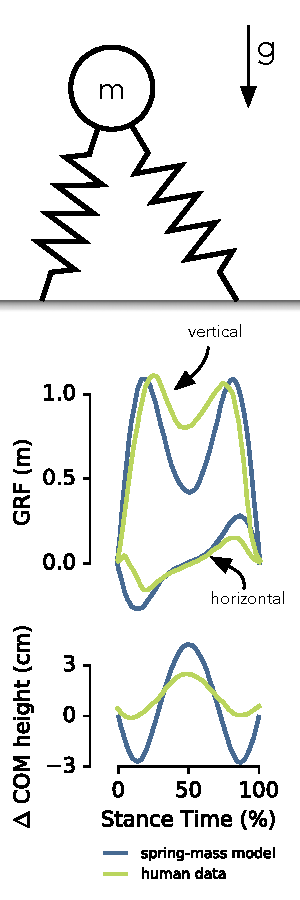
\includegraphics[width=\linewidth]{spring_mass_model_diagram}
    \caption{The bipedal spring mass model captures many fundamental features of
    human walking such as the M-shaped vertical ground reaction profile,
    S-shaped horizontal ground reaction profile and sinusoidal center of mass
    trajectory. Figure adapted from \citet{geyer2006compliant}.}
    \label{fig:ssm_diagram}
\end{marginfigure}

We will look at two paradigms for walking control: centralized approaches that
use full state information and decentralized approaches that use a subset of
state information. Centralized approaches typically utilize a model of the full
system in order to compute control commands that project the full system's
dynamics onto those of the simplified model. Usually, centralized approaches
also place additional constraints on the center of mass (COM) dynamics in order
to facilitate planning and ensure stability. In contrast, decentralized
approaches typically do not explicitly model either the full system or the
fundamental dynamics.  Rather, these approaches use heuristics to generate
motions and forces similar to those of the fundamental model.

\subsection{Centralized Control}\label{sec:back_centralized_control}

\emph{Kinematic centralized control} is one of the oldest forms of locomotion
control. The predominant approach in this category is based on the linear
inverted pendulum model (LIPM) \citep{kajita1991study, kajita20013d}.  This
simplified locomotion model applies additional reductions to the bipedal
spring-mass model, replacing spring legs with ideal prismatic force sources and
constraining the center of mass to move on a plane. The resulting simplified
model features linear COM dynamics with respect to the zero moment point (ZMP).
The ZMP is the point on the ground about the horizontal moments needed to
counteract the total reaction forces on the system is zero. When the ZMP lies
within the support polygon\sidenote{The convex hull of contact points on the
ground} (SP), it is coincident with the center of pressure (COP). On the other
hand, if the ZMP moves beyond the SP, the system will begin to tip over the edge
of the SP. In one dimension, the location of the ZMP is given by, 
\begin{align} 
    x_\textrm{ZMP} = x_\textrm{COM} - \frac{z_\textrm{COM}
        \ddot{x}_\textrm{COM}}{g}. 
    \label{eq:ZMP}
\end{align}
This equation relates the horizontal COM $(x_\textrm{COM})$ dynamics to the
location of the ZMP $(x_\textrm{ZMP})$ given the height of the COM (z_\textrm{COM}

Based on this insight, researchers have developed numerous ZMP-trajectory
methods that follow \labelcref{lipm_step_servo} basic steps:
\begin{steps}
    \item Plan a series of foot steps given the terrain and task such that the
    induced sequence of support polygons contains no
    gaps.\label{lipm_step_foot_plan}

    \item Generate a ZMP trajectory that lies within the support polygons.
    Typically, it is desirable that the trajectory maintains its distance from
    the edges of the support polygons in order to provide a margin of
    stability.\label{lipm_step_zmp_traj}

    \item Solve for the COM trajectory given the desired ZMP trajectory. This
    step requires inverting the solution to a differential equation,
    \cref{eq:ZMP}, to solve for $x_\textrm{COM}$. Researchers have proposed
    numerous solutions to this problem including preview control
    \citep{kajita2003biped}, and differential dynamic programming
    \citep{feng2015optimization}, the latter of which can solve for the ZMP and
    COM trajectories simultaneously.\label{lipm_step_com_traj}
    
    \item Use inverse kinematics to calculate joint velocities that track the
    COM trajectory.\label{lipm_step_ik}

    \item Track the desired joint velocities with servo
    controls.\label{lipm_step_servo}
\end{steps}

A large number of robots have successfully employed this general framework to
walk \citep{hirai1998development}, traverse uneven ground
\citep{shimmyo2010biped}, and run \citep{kajita2007zmp}. Moreover, the method
guarantees that for the nominal gait, the COP will remain in the SP, and thus
the system will maintain its stability.

However, there are several key issues to this approach. One issue stems from
\cref{lipm_step_ik,lipm_step_servo} listed above. These steps generate and
precisely follow via servo control a kinematic trajectory of joint angles. When
perturbed by unforeseen external forces, stiff position control in this manner
may generate large reaction forces and thus may move the COP outside of the SP,
resulting in a fall. We can understand the interactions between the leg and the
environment and the leg and robot body through the concepts of impedance and
admittance. The environment and robot body are admittances, objects that take
forces as inputs and move (or not move) in response. As discussed in
\citet{hogan1985impedance}, it is therefore necessary that the leg acts like an
impedance, an object that produces an interaction force in response to the
position imposed on it by the environment and robot body.

\emph{Dynamic centralized control} seeks to control these interaction forces by
directly computing joint torques, instead of using high-gain position control.
Commonly, in this approach the dynamics model of the full
system\sidenote[][-1in]{Where $q$, $\dot{q}$, and $\ddot{q}$ describe the
generalized coordinates, velocities, and accelerations of the system
configuration, $M(q)$ is the mass matrix, $C(q, \dot{q})$ is a matrix of
centripetal and Coriolis force coefficients, $N(q)$ represents the gravitational
forces, $S$ is a selection matrix that assigns joint torques $\tau$ to
coordinates $q$, $J(q)$ is the Jacobian between joint angles and contact points,
and $\lambda$ is a vector of external forces},
\begin{align}
    M(q) \ddot{q} + C(q, \dot{q}) \dot{q} + N(q) = S\tau + J^T(q) \lambda,
    \label{eq:euler_lagrange}
\end{align}
is used as an equality constraint in a \emph{quadratic program} (QP) that
minimizes torques, reaction forces, and deviation from the desired trajectory.
Additionally, the QP can include inequality constraints representing torque
saturations and friction limits \citep{hutter2013hybrid, herzog2014balancing,
saab2013dynamic, wensing2013generation}. Recently, at the DARPA Robotics
Challenge (DRC) several robots used QP-based dynamic centralized approaches to
control humanoid robots through a disaster relief scenario
\citep{feng2015optimization, kuindersma2014efficiently,
englsberger2014trajectory}. 

While the replacing \cref{lipm_step_ik,lipm_step_servo} with a QP-based torque
control can help improve dynamism and compliance, the resulting biped gaits of
these strategies do not resemble human gaits for two reasons: First, the linear
inverted pendulum model does not produce center of mass trajectories or ground
reaction force profiles similar to those seen during human locomotion.  Second,
human gaits do not constrain the ZMP to the support polygon as we spend
significant time on the heel and balls of our feet during stance
\citep{perry1992gait}.

To overcome these issues and produce more human like gaits, recently researchers
have investigated applying dynamic centralized control approaches to enforce
spring-mass model dynamics instead of LIPM dynamics. With this approach,
researchers have developed robust controllers for both walking
\citep{wensing2013generation} and running \citep{martin2015robust} for humanoid
robots. Alternatively, \citet{sreenath2011compliant} replaced the LIPM model
with a one-degree-of-freedom walking mechanical linkage. In this control, all
joint angles are parameterized with respect to a single phase variable, usually
the leg angle. As the phase variable progresses via its passive dynamics a
control Lyapunov function impose virtual constraints that force joints to follow
a walking gait trajectory. The control expresses a degree of dynamism, as the
phase variable is free to evolve naturally, and demonstrates human-like reflexes
as it is automatically maintains its balance in response to external
perturbations by stepping forward or backwards.

While centralized control approaches have helped close the gap in dynamism and
reactiveness displayed by humans and robotic systems, these methods can also
suffer from their reliance on an accurate model of the system dynamics
(\cref{eq:euler_lagrange}). It may be difficult to identify the parameters of
this model, such as friction and damping coefficients and inertias, especially
for prosthesis systems. Consequently, researchers have explored decentralized
control methods that use only a subset of the state and generally rely on
heuristic control strategies instead of deriving control actions from a detailed
system model. 

\subsection{Decentralized Controllers}\label{sec:back_decentralized_control} 
In contrast to the centralized control methods discussed in the previous
\namecref{sec:back_centralized_control}, decentralized methods generate walking
gaits without requiring measurement of the full system state. Consequently,
decentralized walking strategies typically do not involve
planning\sidenote{\crefrange{lipm_step_foot_plan}{lipm_step_com_traj} of the
centralized control framework} and do not enjoy stability guarantees. Rather,
gait emerges naturally from the coupled dynamics of several closed-loop systems.
In the case of prosthesis control, one system is the human neuromuscular
system and the other is the closed-loop dynamics of the robotic prosthesis.

For example, the earliest robotic prosthesis control strategy, termed \emph{echo
control,} records the kinematics of the healthy leg and then executes an
identical trajectory on the prosthesis on the following step
\citep{grimes1977feasibility, grimes1979active}. This strategy, as with all
robotic prosthesis controls we will review, does not require measurement of the
torso, head, or arm movement. Also, during execution of the trajectory, the
position servo controls only require measurement of the prosthesis joint angles,
making it more practical for implementation on a prosthesis device. However,
this control is an example of a \emph{kinematic decentralized control.}
Consequently, it suffers from many of the same problems identified in
centralized kinematic control. Namely, it does not comply to the environment,
which can result in large and unnatural reaction forces. For example, if a
prosthesis under this control strategy encountered an obstacle during swing, the
knee would not to flex in response, thereby inducing a large moment on the
amputee. Moreover, echo control suffers from the problem of not allowing the
amputee to to start or stop gait with their prosthesis leg.

As was the case for centralized control, commanding torques instead of joint
angles helps alleviate this issue by allowing for compliant interaction with the
environment. \emph{Dynamic decentralized control} typically features a finite
state machine with states representing different phases of gait such as stance
and swing. Within each phase, a heuristic control law specifies the torque
command. For example, the first robotic system to achieve stable, dynamic
locomotion employed simple heuristics to regulate the height, velocity, and
attitude of 2 dimensional one legged hopping robot
\citep{raibert1983dynamically}. Specifically, to control the height of the
robot, the control adjusts the duration of thrust generated by the prismatic leg
actuator during stance. Researchers empirically determined the relationship
mapping thrust duration to hopping apex height. To control horizontal velocity,
first it is assumed that placing the foot in the center of the locus of points
comprised of the center of gravity projected onto the floor will result in zero
change in horizontal velocity. Then, a linear feedback gain on velocity error
determines the offset from this point. A servo control on the leg angle during
swing realizes the desired foot placement. Finally, the control regulates the
torso attitude during stance via PD feedback. 

Unlike a centralized control scheme, \citeauthor{raibert1983dynamically}'s
scheme does not consider the interaction between these control modules,
preferring instead to treat stabilization of each degree of freedom as an
independent task. Regardless, the system demonstrated remarkable dynamism and
robustness, allowing the hopping robot to jump \unit[0.25]{m}, run
\unitfrac[1.2]{m}{s}, and recover from horizontal disturbance forces applied by
an experimenter. Moreover, the control strategy easily extended to 3D locomotion
as well without an exponential increase in computation complexity. This seminal
work demonstrates that LIPM-based, centralized control that carries stability
guarantees is not necessary to ensure stability of robotic systems and suggests
the constraints and model reductions enforced by centralized control may hold
systems back. Rather, intelligent design of heuristic control to shape the
natural dynamics of a system can in fact provide high levels of performance in
practice.

Virtual model control, proposed by \citet{pratt2001virtual}, provides a
convenient method for designing heuristic control strategies. In contrast to the
control proposed in \citet{raibert1983dynamically}, which commands forces
aligned with the robot's actuators, virtual model control does not require such
correspondence. Rather, designers can use their intuition to place virtual
mechanical elements, such as springs, dampers, masses, and linkages on or
between reference coordinate frames located anywhere in space. The virtual
mechanisms apply generalized forces $F$ to the coordinate frames, which are
translated to joint torques $\tau$ via the Jacobian $J$ according to
\begin{align}
    \tau = J^T F.
\end{align}
Joint-level controls realize these desired torques, thereby simulating the
virtual components. 

This control approach has many advantages: First, it provides an intuitive
framework to design controllers for many tasks and many different robot
architectures. Second, even though the original virtual model control proposed
by \citeauthor{pratt2001virtual} is centralized, one can easily design
decentralized controllers with this method as well. If the virtual mechanisms do
not span all the joints, $J$ will be a sparse matrix, resulting in a
decentralized control approach that can be applied to prostheses. Last,
impedance mechanisms such as springs and dampers ensure dynamic interaction with
the environment with reasonable reaction forces.

\subsection{Dynamic Prosthesis Control}
With the goal of dynamic interaction with the environment in mind,
\citet{sup2007design} formulated \emph{impedance control} for active prostheses.
The strategy is a essentially a form of simple virtual model control, where
linear and nonlinear springs along with linear dampers span individual joints.
A finite state machine, such as the one in
\cref{fig:impedance_control_state_flow}, switches impedance functions as the
amputee progresses through phases of gait: early and late stance and early and
late swing. The impedance functions in this strategy actually describe the
\emph{quasi-stiffness} of the joint \citep{rouse2013difference}, which is the
torque vs angle curve seen during walking. Therefore, we will henceforth, refer
to this strategy as quasi-stiffness control for prostheses.

To describe the quasi-stiffness curve, \citet{sup2008design} uses a piecewise
model with linear and cubic stiffness terms, and a linear damping term.
\begin{align}
    \tau = -k_1 (\theta - \theta_0) - k_2 (\theta - \theta_0)^3 - b \dot \theta.
\end{align}
Regression analysis of the torque versus angle and velocity data of intact
subjects performing level-ground walking returns the quasi-stiffness parameters
for each joint in each state. An experimenter can further tune these parameters
to better suit the amputee's gait. 
\begin{marginfigure}
    \centering
    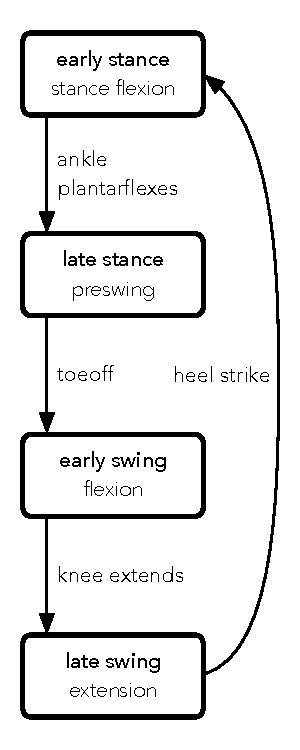
\includegraphics[width=\linewidth]{impedance_control_state_flow}
    \caption{Finite state machine used for the quasi-stiffness control proposed
    by \citet{sup2007design}. In each state the control employs impedance
    functions that determine the behavior of the ankle and knee joints of an
    active transfemoral prosthesis.}
    \label{fig:impedance_control_state_flow}
\end{marginfigure}
This strategy has been implemented on both transtibial \citep{shultz2014walking}
and transfemoral \citep{lawson2014robotic} active prostheses and has improved
amputee gait characteristics over those provided by passive prostheses.
Moreover, by tuning impedance parameters for specific tasks and augmenting the
finite state machine, researchers have extended impedance control to help
amputees to walk up and down slopes \citep{sup2011upslope} and stairs
\citep{lawson2013control}, run \citep{huff2012running, shultz2015running}, and
execute sit-to-stand motions \citep{varol2009powered}.  \citet{lenzi2014speed}
present a similar method, in which a look-up-table directly stores the
quasi-stiffness curve with respect to angle and velocity.  With this method,
\citeauthor{lenzi2014speed} obtain speed adaptation by linearly interpolating
between two look up tables representing slow and fast walking.

In contrast to the kinematic echo control strategy discussed earlier,
quasi-stiffness control should produce more reasonable interaction forces. This
is especially true when the prosthesis encounters an unexpected disturbance, as
the control does not try to follow a specific trajectory with high precision and
thus high feedback gains. However, whereas impedance control as originally
proposed by \citet{hogan1985impedance} advocated independent specification of
the disturbance response torque and the torque required to achieve the desired
motion, the quasi-stiffness control strategies we have discussed use the same
behavior for both. 

Recently, several research efforts have investigated dynamic control strategies
that provide both a feed forward element that generates the desired motion and a
feedback element that responds to disturbances. Such approaches allow one to
tune these these two aspects separately. While these approaches are
decentralized in that they do not require state information of the amputee, they
do borrow aspects of centralized approaches such as trajectory planning, and
model-based computation of feed-forward torques.

For example, \citet{lenzi2014speed, lenzi2014minimum} compute minimum jerk
trajectories for the knee and ankle joints during the swing phase. These
trajectories are parameterized by fifth order polynomials that connect the
initial states of the knee and ankle joints, measured just before toe-off, to to
the desired final states, specified for both joints as zero angle, velocity, and
acceleration. The ankle joint uses a single trajectory, while the knee joint
uses two trajectories, one that connects the initial state to a maximum knee
flexion state and one that connects the maximum knee flexion state to the final
state.  Using a model of the system represented by Euler-Lagrange dynamics
equations (\cref{eq:euler_lagrange}) one can calculate the required feed forward
torque to follow the planned trajectories. Minimizing the jerk, the derivative
of acceleration, helps ensure smoothness of the computed torques. A proportional
derivative feedback control then determines the disturbance response behavior.
The use of a strong feed forward term allows for lower PD feedback gains and
more compliant behavior.

A disadvantage of the minimum jerk trajectory approach is it generates and
executes a trajectory whose duration is heuristically determined at toe-off.
Recently, \citet{gregg2014virtual, zhao2016first} have proposed methods similar
to the centralized virtual constraint control discussed in
\cref{sec:back_centralized_control}, in which the natural progression of a phase
variable determines the rate at which the control follows preplanned
trajectories. \citet{gregg2014virtual} chooses to follow the ankle-foot and
knee-ankle-foot rollover shapes, which are defined as the location of the center
of pressure with respect to coordinate systems attached to the shank and the
ankle-hip line respectively. The center-of-pressure naturally becomes the phase
variable for these trajectories. The observation that the roll-over shapes are
invariant across walking speed, shoe geometry, and amputee weight motivates this
choice. In this strategy, a model-based feedback linearization controller
enforces adherence to these desired trajectories as the center of pressure
progress through its natural dynamics. This formulation provides both the feed
forward torque command and a disturbance response command that provides
exponential converge to the desired rollover shapes. 

As we noted earlier for centralized robotic control approaches, a downside of
these two trajectory following controllers is their reliance on accurate
dynamics models to compute feed forward torques. To overcome this issue,
\citet{zhao2016first} propose a model-independent virtual constraint control. In
this scheme, quasi-stiffness control provides a feed-forward torque signal that
reduces the dependence on the model. A quadratic program then computes the
minimum required extra effort to ensure convergence to a preplanned trajectory
that is parameterized with respect to hip angle.

\section{Bioinspired Control for
Prostheses}\label{sec:back_bioinspired_pros_control} 

The dynamic control prosthesis control strategies we outlined in the previous
section in some sense all provide a feed-forward torque that generates a desired
nominal trajectory, and an impedance behavior that determines the disturbance
response characteristics. In the case of quasi-stiffness control, the same
function encodes both of these characteristics.  In the case of trajectory
following controllers, model inversion provides the necessary torque to execute
the plan while either a proportional derivative controller, feedback
linearization, or control Lyapunov function provides impedance behavior.
However, it is not clear that these approaches generate the impedance responses
of the system we actually want to replicate in the field of prosthetics, that of
the amputee's missing limb. In the biological leg, impedance characteristics may
play a crucial role when it comes to stabilizing movement
\citep{won1995stability, burdet2001central} and changes in response to a number
of factors including any of mean ankle torque, ankle position, perturbation
amplitude, and muscle fatigue \citep{kearney1989system}.

An alternative approach to developing prosthesis control, which may better model
joint quasi-stiffness and joint impedance, is to model the underlying biological
neuromuscular dynamical system that gives rise to these characteristics. Two
hypothesized mechanisms that govern the neuromuscular system are central pattern
generators (\cref{sec:back_CPG}) and reflexes
(\cref{sec:back_neuromuscular_reflexes}). These two mechanisms are naturally
decentralized and dynamic and are thus attractive models to utilize in a
prosthesis controller.

\subsection{Central Pattern Generators}\label{sec:back_CPG}
\subsubsection{Central Pattern Generators in Biology}
\emph{Central Pattern Generators} (CPGs) are hypothesized nonlinear
oscillators, comprised of neurons in the central nervous system, that can
autonomously generate periodic neural activation
patterns~\citep{ijspeert2008central}.  \citet{brown1911intrinsic} first
suggested their existence based on experiments he conducted on decerebrated and
deafferented cats. In these experiments, \citeauthor{brown1911intrinsic} severed
both the afferent pathways (that carry sensory information) and efferent
pathways (that transmit higher level commands from the brain to motor neurons).
Despite the lack of high level control and sensory feedback, the cats still
displayed cyclical motions in their hind legs similar to those seen during
normal gait. This result suggests CPGs may play an important role in generating
locomotion controls in vertebrate animals. Similar cyclical neural activity
(called fictive locomotion) has been found in isolated lamprey spinal cords
\citep{cohen1980neuronal}, salamanders \citep{delvolve1999fictive}, and frog
embryos \citep{soffe1982tonic}. 

\begin{marginfigure}
    \centering
    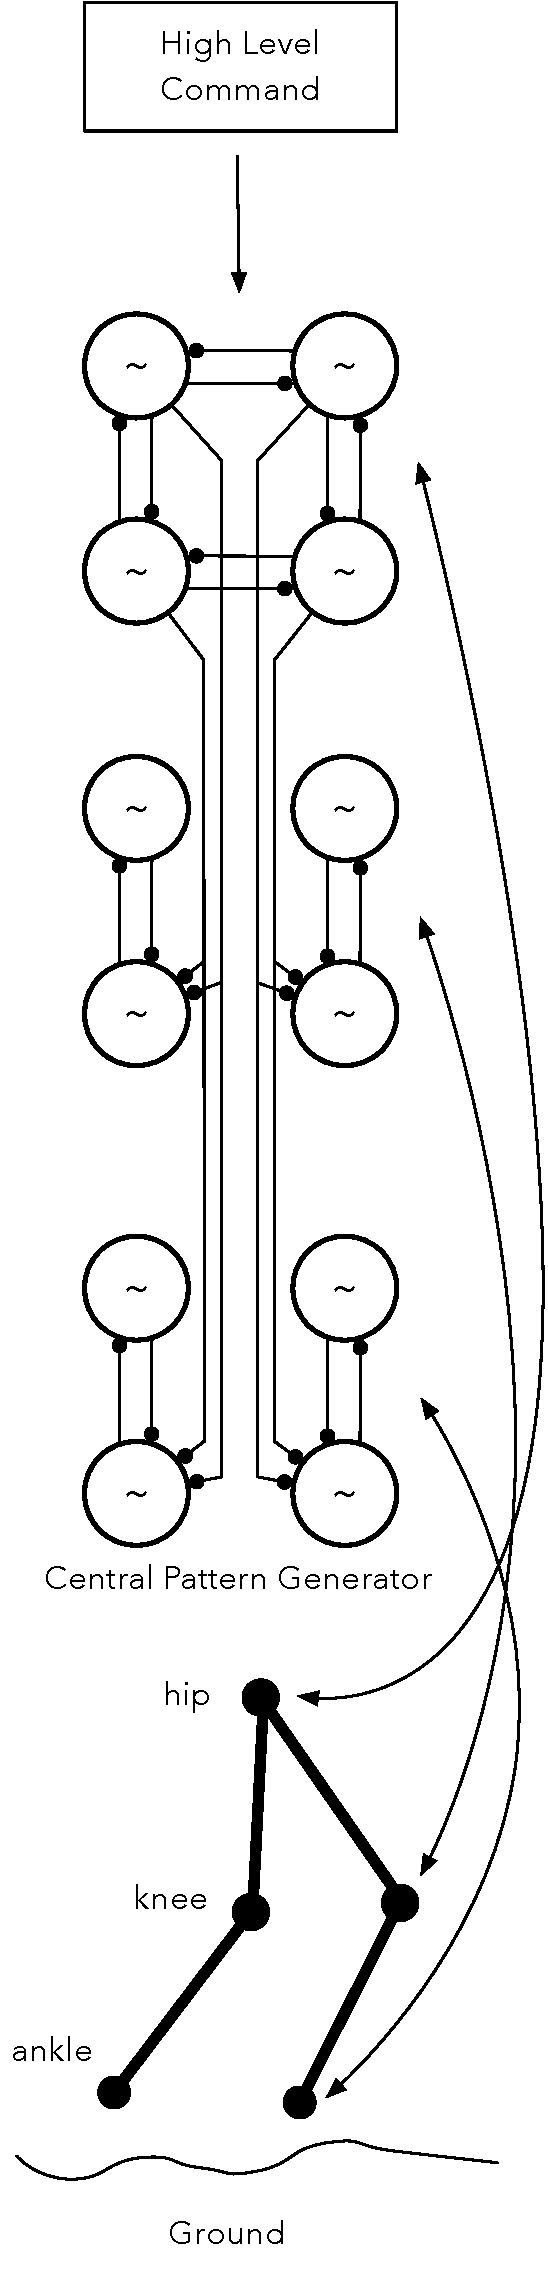
\includegraphics[height=6.25in]{CPG_diagram}
    \caption{Central Pattern Generator for bipedal locomotion as described in
    \citet{taga1991self}. Six neural oscillators receive feedback from and
    command joint torques for the hips, knees, and ankles of a planar biped
    model. A one dimensional high-level control signal enables control of speed
    and elicits gait transitions.}
    \label{fig:cpg_diagram}
\end{marginfigure}
Moreover, research has shown that stimulation of a region of the brain stem
called the Mesencephalic Locomotor Region (MLR) can manipulate the neural
activity generated by CPGs. For example, electrical stimulation of the MLR led
to gait transitions in both decerebrated cats \citep{shik1966control} and
salamanders \citep{cabelguen2003bimodal}.  Therefore, CPGs may serve as a form
of dimensionality reduction and decentralization for the biological control
system as low-dimensional, high-level signals from brain can shape the
high-dimensional, low-level CPG output. Consequently, CPGs may also represent
an attractive option for robotic legged locomotion controllers as
decentralization and dimensionality reduction are desirable properties in this
domain as well.

\subsubsection{Neuromechanical Models with CPGs}
The seminal work on CPG-based bipedal locomotion control is presented in
\citet{taga1991self}. In this model, a CPG neural network of six interconnected
oscillators describes the joint torques applied to a four link biped model.
Differential equations, first presented in \citet{matsuoka1987mechanisms} with
additional sensory feedback from joint and inertial link angles, describe the
output of the CPG network. The resulting biped model walks with a natural gait
featuring both single and double support and demonstrates robustness to a
variety of disturbances including changes to ground stiffness, damping, and
slope. Additionally, tuning a single parameter induced a transition from walking
to running in the model in a manner comparable to the biological gait
transitions observed after stimulation of the MLR.

CPGs have successfully controlled several bipedal humanoid robots. For example,
\citet{endo2005experimental} used \citeauthor{matsuoka1987mechanisms}'s
nonlinear oscillators along with by bio-inspired feedback pathways that regulate
ground reaction forces and body roll to generate desired foot trajectories for
the bipedal QRIO robot. As in \citeauthor{taga1991self}'s simulations walking
speed can be controlled via adjustment of a single parameter and the robot is
robust to changes in step height. Authors have also successfully employed other
nonlinear oscillator models. In \citet{shan2002neural}, a Recurrent Neural
Network generates oscillatory signals for a 20-DOF humanoid robot, HOAP-1, that
allow it to walk up and down stairs. In \citet{righetti2006programmable},
programmable ``Hopf'' oscillators \citep{righetti2006dynamic} learn desired
walking trajectories through entrainment enabling HOAP-2, a 25-DOF robot, to
walk forwards and backwards at varying speeds and step lengths.  

\subsubsection{CPGs for Prosthesis Control}
CPGs have also been proposed for controlling both mechanically-passive and
active lower limb prostheses.  \citet{nandi2009development} optimize CPG
parameters to fit recorded knee angle trajectories from healthy human subjects.
During walking, the CPG entrains desired knee motions to the oscillations of the
amputee's hip joint. The desired knee angles are achieved in a
mechanically-passive prosthesis via online adjustment of the knee damping.
Similarly, \citet{torrealba2010through, mora2012cybernetic} also use a CPG to
control a mechanically-passive variable damping prosthesis but use phase
resetting to synchronize the amputee and CPG dynamics. 

For active prostheses, \citet{geng2012design} suggest using a Hopf oscillators
to fit the trajectory of the knee angle during walking. \citet{guo2010study}
extend the idea of using a CPG for active prosthesis control by proposing a
hierarchical approach with a support vector machine (SVM) at the high-level
inferring amputee intent from EMG signals, and a CPG at the lower-level
determining the desired knee and ankle angles for an active transfemoral
prosthesis. However, in both cases, the authors do not provide experimental
results on real prosthesis hardware. Moreover, unlike in
\citeauthor{taga1991self}'s original work, these proposed CPG networks for
prostheses generate desired joint kinematics instead of torques. Consequently,
these controllers may not allow prostheses to exhibit the dynamism and
compliance we desire.

\subsection{Neuromuscular Reflexes}\label{sec:back_neuromuscular_reflexes}
\subsubsection{Neuromuscular Reflexes in biology}
Around the same time \citeauthor{brown1911intrinsic} hypothesized the existence
of central pattern generators, \citet{sherrington1910integrative,
sherrington1910flexion} suggested another mechanism for oscillatory neural
signals: chains of \emph{reflexes}, or local feedback loops, that trigger in
response and entrain to sensory signals. \citeauthor{sherrington1910integrative}
identified complex, multi-joint, multi-limb reflex arcs involving both
excitation and inhibition in response to cutaneous stimulation in decerebrated
cats. Moreover, he observed rhythmic stepping behavior in decerebrated cats
suspended off the ground and concluded that the behavior emerged reflexively
based on proprioceptive signals emanating from the muscles themselves and not
from centrally generated oscillatory signals.

In animal experiments discussed earlier, while CPGs can go a long way towards
explaining locomotion neural activity, they still do not fully explain all
observed phenomena. Reflexes likely at least shape locomotion activation
patterns through entrainment, for example in Lamprey's movement of the tail
generates activation in the spinal chord of equal frequency
\citep{mcclellan1993mechanosensory}, and phase resetting, as demonstrated by the
ability of decerebrated cats to walk on treadmills across a range of speeds
\citep{rossignol2000locomotion}.

For human and primate bipedal locomotion, the role of CPGs is more muddied and
the role of reflexes more evident than for decerebrated cats and simpler
vertebrate animals \citep{mackay2002central, vaughan2003theories,
nielsen2003we}. This is perhaps due to the demands of controlling the inherently
unstable dynamics of upright walking \citep{capaday2002special}. For example,
while rhythmic spinal activity has been observed in humans, it is not clear if
the neural signals are an example of autonomous fictive motion, indicative of a
CPG, or entrainment with stretch reflexes in leg muscles
\citep{capaday2002special, stewart1991modulation}. In this case, we can also
look to robotics to provide insight about biology: in the previously discussed
experiments on humanoid robots controlled by CPGs, a significant reduction in
robustness was observed after blocking sensory feedback pathways
\citep{endo2005experimental, righetti2006programmable} indicating CPGs alone may
not fully explain bipedal locomotion. Whereas research has not yet clearly
established the presence of a CPG driving human locomotion, research has
identified many reflexes that contribute to locomotion such as the Hoffman
reflex (H-reflex) of the soleus ankle plantarflexor muscle
\citep{capaday1987difference}, stretch reflex in the soleus
\citep{yang1991contribution}, soleus force feedback \citep{grey2007positive},
and cutaneous reflexes that induce withdrawal responses \citep{yang1990phase}. 

\subsubsection{Neuromuscular Models with Reflexes}
To model the potential interplay between muscular reflexes and CPGs in human
locomotion \citet{ogihara2001generation} extend the model presented in
\citet{taga1991self} by adding muscles stimulated by alpha motor neurons. This
model simulates nine muscles of the leg, each stimulated by an alpha motor
neuron that receives input from a CPG oscillator and proprioceptive feedback
from one or more muscles. The muscles produce forces according to their state
and activation input (computed using models presented in
\citet{pierrynowski1985physiological} and \citet{davy1987dynamic}). These forces
are applied to constant moment arms in order to produce joint torques summed
about joints as in a virtual model control. The authors optimize the cost of
transport of transport of the biped with a genetic algorithm and achieve a gait
with human-like kinematics and kinetics. Moreover, the forces produced by many
of the muscles resemble those produced during human locomotion. Despite the fact
that the CPG used in this model received no feedback signals, the resultant gait
still exhibited a small degree of robustness to perturbations although not as
much as \citeauthor{taga1991self}'s model. The author's attribute the robustness
to the stabilizing feedback provided by muscle reflexes. 
\begin{marginfigure}
    \centering
    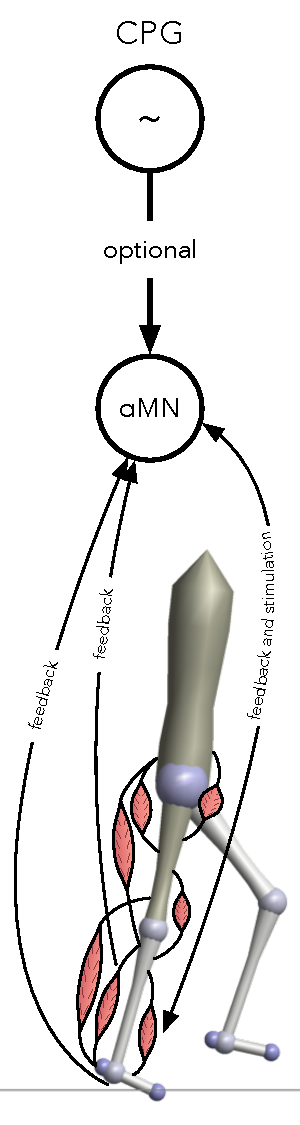
\includegraphics[height=5.5in]{reflex_diagram} 
    \caption{Neuromuscular models with reflex feedbacks. The model developed by
    \citet{ogihara2001generation} activates individual muscles according to the
    activity of a CPG and proprioceptive reflexes that can involve the muscle
    itself, other muscles, and ground contact sensing.  \citet{geyer2010muscle}
    does away with the CPG and achieves locomotion with only reflex feedbacks.}
    \label{fig:reflex_diagram}
\end{marginfigure}

Whereas models and robot experiments show reflexes are vital for maintaining
bipedal gait stability, the same cannot be said about CPGs. In fact, as shown by
\citet{geyer2010muscle}, it is possible to simulate robust and human-like
bipedal locomotion using only reflexes. This work employs a neuromuscular
model, similar to that used in \citet{ogihara2001generation}, but does away with
the feed forward CPG stimulations sent to alpha motor neurons. Instead,
\citeauthor{geyer2010muscle} hypothesize the existence of several force and
length muscle reflexes that implement three key aspects of bipedal locomotion:
compliant leg behavior, preventing joint over extension, and providing trunk
stabilization. The gait achieved by this model is more robust than and more
accurately reproduces kinematics, kinetics, and ground reaction forces seen in
human walking than \citeauthor{ogihara2001generation}'s model. Moreover, it also
produces human-like stimulations for many of its muscles.

While we cannot say based on this result alone that CPGs do not play an
important role in human locomotion, the fact that human locomotion can emerge
from purely reflexive controls increases the attractiveness of using this
approach for prosthesis control. The reflex-only paradigm may be easier to
design and optimize than the CPG+reflex paradigm for two reasons: First, the
reflex connection graph used by \citet{geyer2010muscle}'s reflex-only model is
much more sparse than that used by \citet{ogihara2001generation} CPG+reflex
model. Using a sparse set of reflexes and no CPG reduces the number of
parameters that we must tune in order to achieve locomotion. Second, the
reflexes in the reflex-only model are functionally motivated, which may increase
our intuition about the role of each reflex and assist our ability to tune the
model's parameters. This is evidenced by the fact that
\citeauthor{geyer2010muscle} hand tuned the parameters of their model whereas
\citeauthor{ogihara2001generation} used a genetic algorithm.  Moreover,
functionally motivated feedbacks used in the reflex-only approach has allowed
further research to extend this model to include swing leg placement
\citep{desai2013muscle}, 3D locomotion, running, speed changes, stair and slope
negotiation, turning, and obstacle avoidance \citep{song2015neural}.  

The robustness properties exhibited by neuromuscular model are especially
relevant to our goal of developing a robust prosthesis control that will help
transfemoral amputees avoid falls. In \citet{song2015neural} the author's
improve the model's robustness by incorporating reflexes that place the swing
leg into target landing angles. The authors optimize this model to achieve a
combination of robustness and energy efficiency.  The resulting gait can walk on
terrains featuring random steps up to $\unit[\pm 6]{cm}$ (50 \% success rate)
and rejects pushes in both the forward and backward directions at various points
in the gait cycle. In another work, \citet{murai2011neuromuscular} subject a
neuromuscular model, initially trained to match kinematic data of single
subject, to impacts during early and late swing. They find the learned model
exhibits the elevating and lowering trip response strategies of the biological
leg despite not being explicitly trained to do so. These disturbance response
characteristics point to reflex control providing the appropriate quasi-static
and impedance behaviors.

\subsubsection{Neuromuscular Reflexes for Prosthesis Control}
\begin{marginfigure}
    \centering
    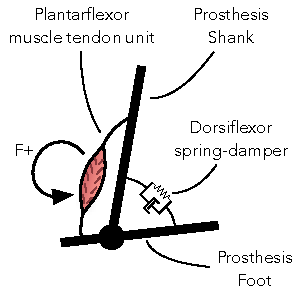
\includegraphics[width=\linewidth]{eilenberg_diagram} \caption{Neuromuscular
    model used by \citet{eilenberg2010control} to control an active ankle
    prosthesis. During stance, a virtual muscle driven by positive force
    feedback, generates plantarflexion torque. During swing, a virtual spring
    damper provides dorsiflexion torque to prevent toe scuffing.}
    \label{fig:eilenberg_diagram}
\end{marginfigure}
Motivated by the robustness and natural gait achievable by neuromuscular
reflex control, past research has applied this model to active prostheses and
exoskeletons. \citet{eilenberg2010control} applied a simplified version of the
control to a powered ankle prosthesis (\cref{fig:eilenberg_diagram}). In this
work, the neuromuscular model was reduced to a single ankle plantarflexor muscle
driven by a positive force feedback reflex during stance. During swing, the
control applies torque to dorsiflex the ankle according to a virtual spring
damper model. In amputee testing of a prosthesis controlled by the neuromuscular
model the control produced ankle kinematics and kinetics similar to those
observed in healthy human walking. Significantly,
\citeauthor{eilenberg2010control} found evidence that the robustness and
entrainment properties observed in neuromuscular model simulations may carry
over to amputee gait as well. The author's note that the prosthesis
automatically adapts torque output when walking on slopes, producing more
plantarflexion torque when walking up slopes and less when walking down slopes.
Additionally, \citet{markowitz2011speed} found that a similar neuromuscular
reflex model automatically produced more ankle plantarflexion work as the
amputee increased his gait speed.

\subsubsection{EMG-based Control}\label{sec:back_emg_control}
The inclusion of user intent recognition via surface electromyography (EMG)
signals represents an interesting extension of neuromuscular reflex prosthesis
control. In these approaches, muscle activity in the residual limb is directly
measured via EMG sensors embedded in the amputee's prosthesis socket. These EMG
sensors are then used to control the torque generation of the amputee's leg
prosthesis. Because neuromuscular models describe how joint torque is generated
in response to muscle activations, a natural approach is to use the EMG signal
in reflex pathways in order to activate virtual muscles. This is the approach
proposed by \citet{wu2011electromyography}. In this work,
\citeauthor{wu2011electromyography} control an active transfemoral prosthesis
using EMG sensor readings from the residual thigh to activate virtual knee
flexor and extensor muscles according to a linearised Hill muscle model. The
resulting prosthesis control allowed an intact subject wearing the prosthesis
via an able-bodied emulator to achieve nearly normal gait. In a similar
approach, \citet{wang2013proportional} use EMG signals to modify the gain on a
positive torque feedback loop (similar to positive force feedback used in
\citet{geyer2010muscle}) in order to control ankle plantarflexion torque. As
seen in healthy human walking, toe off angle and ankle net work increased with
increasing walking speed.

These two works have demonstrated that neuromuscular approaches have enabled EMG
based control to go beyond its typical application of high-level mode
recognition. For example, \citet{huang2009strategy, huang2011continuous}, and
\citet{hargrove2015intuitive} recognize walking modes, such as level ground
walking, ramp and stair ascent, and ramp and stair descent, by training
classifiers on features of EMG and mechanical sensor data. In contrast, the EMG
+ neuromuscular approaches allow the use typically noisy EMG sensor data for
low-level continuous control. \citet{wu2011electromyography} and
\citet{wang2013proportional} propose that because EMG + neuromuscular approaches
model physiologically plausible feedback loops and dynamics, they may allow
amputees to use muscle activations to control their prostheses in an intuitive
way.

\subsection{Conclusion} 
In summary, simulations and implementations of the neuromuscular reflex control
approach have repeatedly demonstrated its ability to generalize to a variety of
situations and exhibit robustness to a variety of disturbances. Due to the gait
deficits and fall risk transfemoral amputees face, these two properties make
this control paradigm very attractive for application to transfemoral prostheses
. Moreover, neuromuscular approaches have been successfully extended with EMG
sensor feedback from amputees' residual limbs, enabling intuitive low-level
prosthesis control. In contrast, other control approaches for prostheses such as
quasi-stiffness control have not demonstrated these properties. Importantly,
neuromuscular control addresses \cref{chal:dynamic,chal:incomplete_state} of
amputee locomotion~(\cref{sec:intro_challenges}) as we can implement them via a
decentralized, sparse set of reflexes and they allow for dynamism by providing
both a quasi-stiffness and impedance response via the dynamics of the
stimulated muscle models..

As yet, there have not been any published works applying neuromuscular reflex
control to active knee and ankle transfemoral prostheses. Therefore, in this
thesis, we work towards this goal with the hope of improving transfemoral
amputee gait robustness and naturalness. \Cref{sec:neuro_model} will review the
details of the particular neuromuscular implementation used in this thesis.

\section{Prosthesis Design}\label{sec:back_pros_design}
We can trace efforts to build an active knee-ankle prostheses to the seventies
when \citet{flowers1974use} created an active knee-ankle prosthesis emulator in
order simulate potential control schemes. This prosthesis used a hydraulic
actuator capable of producing $\unit[90]{N \cdot m}$ of torque and
$\unitfrac[0.5]{rev}{s}$ of no-load speed, sufficient for simulation of passive
prostheses. With this device, \citet{donath1974proportional} tested proportional
EMG control, a problem researchers are still investigating today
(see~\cref{sec:back_emg_control}). Indeed, this line of research proved to be
far ahead of its time, as most relevant research in active lower-limb prostheses
design has occurred only in the last ten years. The recent interest in active
knee ankle prostheses has been spurred by hardware improvements that allow
designs to approach the strength, speed, and low weight of the biological leg.
Enabling technologies include power-dense brushless motors, motor controllers,
and lithium-ion batteries, inexpensive microcontrollers and inertial measurement
units (IMUs), and strong but light composite materials such as carbon fiber.
With these advancements, engineers have successfully designed prostheses to meet
or exceed the requirements for walking~(\cref{tab:walking_requirements}).
\begin{margintable}
  \centering
  \begin{tabular}{lll}
    \toprule
    & Ankle Max & Knee Max \\
    \midrule
    Velocity & \unitfrac[0.72]{rev}{s} & \unitfrac[1.17]{rev}{s}\\
    Torque & $\unit[130]{N \cdot m}$ & $\unit[57]{N \cdot m}$\\
    Power & \unit[350]{W} & \unit[120]{W}\\
    \bottomrule
  \end{tabular}
  \caption{Required knee and ankle torque, velocity, and power for walking
  (\unitfrac[1.40]{m}{s} average speed, scaled to \unit[85]{kg} subject,
  data from \citet{winter2009biomechanics})}
  \label{tab:walking_requirements}
\end{margintable}

In this \namecref{sec:back_pros_design}, we review a number of recent prosthesis
designs and analyze their ability to enable dynamic locomotion
(\cref{chal:dynamic,chal:incomplete_state} of transfemoral prosthesis locomotion).  To address
this challenge, prostheses should be able to regulate their output joint torques
and behave as though they have inertial properties similar to that of a normal
human leg. This will ensure that the prosthesis will emulate the energy
efficient gaits of normal walking and remain compliant to unforeseen
disturbances and uneven terrain.

\subsection{Direct Drive Transfemoral Prostheses}\label{sec:back_direct_drive}
\begin{marginfigure}
    \centering
	\begin{subfigure}[t]{\linewidth}
    	\centering
        %\includegraphics{}
        \missingfigure{Gen 1}
        \caption{Generation 1 used ball screw transmissions, \unit[200]{W}
        brushless motors, and a unidirectional parallel spring in the ankle that
        reduced motor torque requirements \citep{sup2009preliminary}.}
        \label{fig:vanderbilt_gen_1}
	\end{subfigure}

	\begin{subfigure}[t]{\linewidth}
    	\centering
        %\includegraphics{}
        \missingfigure{Gen 2}
        \caption{Generation 2 replaced ball screws with custom gear-based
        transmission that is less noisy and more durable
        \citep{lawson2013control}.}
        \label{fig:vanderbilt_gen_2}
	\end{subfigure}

	\begin{subfigure}[t]{\linewidth}
    	\centering
        %\includegraphics{}
        \missingfigure{Gen 3}
        \caption{Generation 3 features a modular design with separable knee and
        ankle units \citep{lawson2014robotic}.}
        \label{fig:vanderbilt_gen_3}
	\end{subfigure}
    \caption{Vanderbilt University's Robotic Transfemoral Prostheses.}
    \label{fig:vanderbilt_prostheses}
\end{marginfigure}

The most common approach for active transfemoral prosthesis design employs
electric motors, coupled to transmissions, that directly drive the knee and
ankle joints. The transmissions may utilize a combination of gears, chains,
belts, ball screws, and four-bar-mechanisms in order to increase the torque
output of the actuator, at the expense of speed, in order to satisfy the
requirements listed in \cref{tab:walking_requirements}. A successful line of
transfemoral prostheses following this design paradigm comes from Vanderbilt
university. The first prosthesis in this line \cref{fig:vanderbilt_prostheses}a
used a pair of ball screw transmissions and brushless motors capable of
\unit[200]{W} of continuous power output to drive its knee and ankle joints
\citep{sup2009preliminary}. 

With these actuators, the knee motor can achieve the required peak torque and
peak power intermittently (\cref{tab:walking_requirements}). However, the ankle
motor may be overly stressed due to the high requirements of walking. To remedy
this, this prosthesis includes of a unidirectional parallel spring in the ankle
that reduces the required ankle motor torque. As shown in figure
\cref{fig:ankle_torque_vs_angle}, during level ground walking, a linear torsion
spring accounts for a significant portion of the ankle's torque versus angle
relationship. Therefore, incorporating a spring into the ankle offloads this
portion of the torque from the motor. The ankle motor only needs to provide the
delta between the desired output torque and the linear spring. As a result, the
spring reduces motor energy consumption, heat generation, and transmission wear.

Further improvements resulted in two more generations of prostheses
(\cref{fig:vanderbilt_gen_2,fig:vanderbilt_gen_3}) \citep{lawson2013control,
lawson2014robotic}. These versions replaced ball screw transmissions with
a multi-stage belt/chain due to the improved packaging and reduced noise and
wear they afford (Michael Goldfarb, personal communication, September 18, 2013).
With these prostheses, researchers have extensively tested a variety of control
strategies including quasi-stiffness control \citep{sup2009preliminary,
sup2011upslope, lawson2013control, lawson2014robotic, lenzi2014speed}, EMG-based control
\citep{ha2011volitional, varol2010multiclass}, minimum jerk trajectory following
\citep{lenzi2014minimum}, and virtual constraint control
\citep{gregg2014virtual}. 

Additional prostheses in the direct drive category include AMPRO
\citep{zhao2016first}, and a commercially available active knee and ankle
prostheses: the Össur Power Knee and Proprio Foot. The AMPRO prosthesis features
two 374 W motors coupled to Harmonic Drive transmissions.
\citet{zhao2016first}, use this prosthesis to asses the merits of a virtual
constraint controller. The Össur Power Knee features an electric motor that can
provide torque to facilitate sit-to-stand motions, stair climbing, and active
extension and flexion during walking. The Proprio Foot also features electric
actuation that allows it to adapt to terrain and dorsiflex the ankle during
swing to help avoid trips. 
\begin{marginfigure}
    \centering
    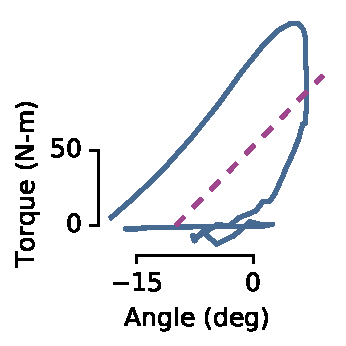
\includegraphics[width=\linewidth]{ankle_torque_vs_angle}
    \caption{Torque vs angle relationship for the ankle during level ground
    walking. A linear spring relationship captures a significant portion of
    ankle function during stance. Data from \citet{winter2009biomechanics}
    scaled to 85 kg subject.}
    \label{fig:ankle_torque_vs_angle}
\end{marginfigure}


\subsubsection{Torque Control Strategies for Direct Drive Prostheses}
In order to achieve dynamic locomotion capabilities, it is crucial that
prosthesis designs allow for closed loop control of torques. To do this control
system must be able to accurately measure the torque at the joint output. There
are two main strategies for torque measurement used by direct drive prostheses.

The first strategy is to measure the current draw of the motors windings, which
is related linearly to the motor torque. One can then multiply this measurement
by the gear ratio to obtain an estimate of the output joint torque. This is the
method used by Generations 2 and 3 of the Vanderbilt prosthesis as well as the
AMPRO prosthesis. The benefit of this method is that it utilizes existing
hardware and allows one to use high frequency current control modes of motor
drivers. However, a drawback of this method is that it measures the torque
before the transmission. Consequently, it does not account for frictional
losses, which can be difficult to model, especially for geared systems. A
strategy that deals with this problem is to install load cells in series with
the motor after the transmission, as was done on Generation 1 of the Vanderbilt
prosthesis. With this method, the closed-loop control can compensate for
frictional losses as they are included in the torque measurement. 

However, this method may still not address a second problem: sluggish passive
dynamics caused by reflected inertia and damping. Reflected inertia refers to
the apparent magnification of motor rotor and gearing inertia on the outside of
gearbox.  We can derive this effect through Newton's second law for the geared
motor
\begin{align}
    J_i \ddot{\theta}_i = \tau_i - b_i \dot{\theta}_i.
\end{align}
Here, $\theta$ and its derivatives refer to angular states of the motor, $b$
is the damping constant, $J$ is the inertia and $\tau$ is the motor torque. We
use subscript $i$ to refer to these quantities as seen before the gear
reduction, and subscript $o$ to refer to those quantities reflected outside of
the motor. Plugging in $\theta_i = n \theta_o$ and $\tau_i = \frac{1}{n}
\tau_o$, where $n$ is the gear ratio, and multiplying through by $n$ yields
\begin{align}
    J_i n^2 \ddot{\theta}_o &= \tau_o - b_i n^2 \dot{\theta}_o \\
    \implies \quad J_o \ddot{\theta}_o &= \tau_o - b_o \dot{\theta}_o.
\end{align}
These equations show that the inertia and damping of the motor rotor are
amplified by the square of the gear ratio. As prostheses may often use gear
ratios in excess of 100:1, this effect can be substantial. 

\begin{table}
  \centering
  \begin{tabular}{lll}
    \toprule
    & Knee & Ankle \\
    \midrule
    rotor inertia & $\unit[0.035]{kg \cdot cm^2}$ 
        & $\unit[1.210]{kg \cdot cm^2}$\\
    gear ratio & 176:1 & 115:1 \\
    reflected inertia & $\unit[0.11]{kg \cdot m^2}$ & 
        $\unit[1.6]{kg \cdot m^2}$\\
    human inertia & $\unit[0.66]{kg \cdot m^2}$  & $\unit[0.019]{kg \cdot m^2}$\\
    percent increase & 17\% & 8400\% \\
    \bottomrule
  \end{tabular}
  \caption{Estimated reflected inertia at knee and ankle joints of Generation 3
  Vanderbilt Prosthesis \citep{lawson2014robotic}. Motor data taken from Maxon
  Motors Catalog\citep{maxon_flat_motor,
  maxon_ec4pole} Knee reflected inertia compared to inertia of human shank and
  foot about knee. Ankle inertia compared to human foot about its center of
  mass. Human inertias estimated from \citet{winter2009biomechanics} for an
  \unit[85]{kg}, \unit[1.7]{m} tall person.}
  \label{tab:vanderbilt_reflec_interita}
\end{table}

For example, \cref{tab:vanderbilt_reflec_interita} shows the calculated
reflected inertias of the Maxon Motors used in Generation 3 of the Vanderbilt
prosthesis and compares the values to the estimated inertia of the shank and
foot about the knee and the foot about its center of mass. We see that at the
knee, the reflected inertia is roughly 17\% of that of the human shank and foot.
In practice, this value is likely several times higher after including the
inertia of the encoder, bearings, and gearing. Consequently, we can estimate
that the reflected inertia may be on the order of the leg itself. At the ankle,
the reflected inertia of the rotor alone is several orders of magnitude more
than that of the foot and more than twice that of the shank and foot. When we
also consider reflected damping and friction, the dynamics of prosthesis system
may be significantly slower than assumed.

The increase in joint impedance created by transmissions could present an issue
when attempting to execute dynamic behaviors involving impact such as running or
trip recovery. In an impact event, the impulse will move through the system at
the speed of sound through metal, roughly \unitfrac[6420]{m}{s} for aluminum
\citep{lide2004crc}. If the prosthesis is \unit[0.5]{m} long, the shock will
traverse its length in \unit[0.00008]{seconds}. This is about 10 times faster
than the typical \unit[1000]{Hz} control frequency of prosthesis control
systems, rendering closed loop torque control with load cells unresponsive. The
impact shock could cause damage to gearing and discomfort for the amputee.

%Reflected Inertia
%Vanderbilt gen 3 ankle = 1210 g*cm^2 * 115^2 in kg*m^2 = 1.6 kg*m^2
%Vanderbilt gen 3 knee = 35 g*cm^2 * 176^2 in kg*m^2 = 0.11 kg*m^2

%human leg for 1.7 85 kg = 0.6575 kg*m^2
%human foot for 1.7m 85 kg = 0.0187 kg*m^2

\subsection{Design of Dynamic Prostheses}
In contrast to the direct drive actuation discussed in the previous subsection,
prostheses that employ series elastic actuation may be better poised to achieve
dynamic locomotion \citep{pratt1995series}. This actuation scheme (illustrated
in \cref{fig:sea_diagram}) aims to solve the torque measurement and impedance
amplification caused by transmissions by placing a spring in series with the
actuator. Measuring the deflection of the spring allows for accurate closed-loop
control of the joint torque. Moreover, the spring low-pass filters external
impulses, granting the control system more time to move the motor rotor in
response to the external load.  Due to these properties, designers have
integrated series elastic actuators into a number of bipedal robots that seek to
achieve dynamic locomotion such as M2V2 \citep{pratt2008design} and ATRIAS
\citep{grimes2013atrias}.

\begin{marginfigure}
    \centering
    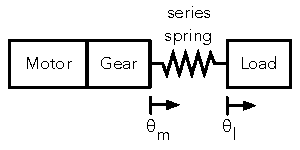
\includegraphics[height=6.25in]{sea_diagram}
    \caption{Series elastic actuation inserts a spring between the gear output
    and the load (here drawn as linear actuator for simplicity). Torque is
    measured via the spring deflection, $\tau = k(\theta_l - \theta_m -
    \theta_0)$ where $\tau$ is the output joint torque, $k$ is the spring
    constant, and $\theta_l$ and $\theta_m$ are the load and motor positions and
    $\theta_0$ is the spring's rest length.}
    \label{fig:sea_diagram}
\end{marginfigure}

Series elastic actuators have found use in a variety of transtibial and
transfemoral prostheses. We can further split these applications into two
categories, those that optimize the spring stiffness for control bandwidth
subject to shock tolerance and those that optimize spring stiffness to optimize
efficiency.

\subsubsection{Springs for Bandwidth and Shock Tolerance}
Adding a spring between the gear and load introduces additional dynamics between
external torques and torques applied to the gearbox as external torques must
physically displace the load before they generate torque on the motor. This
property can improve the shock tolerance of SEA actuators over that of direct
drive motors~\citep{robinson2000design}. However, by the same token, the SEA
also introduces additional dynamics between motor torque and load torque, hence
reducing force control bandwidth. Therefore, a trade-off exists between the
compliance of the actuator and speed with which it can generate desired torques.

\citet{au2007biomechanical, au2008powered} design powered ankle prostheses with
this trade off in mind. In these publications, the authors find that using an
SEA spring soft enough to protect the ball screw transmission results in
insufficient closed loop torque control bandwidth. To overcome this shortcoming,
the authors incorporate a parallel spring into the ankle as was done for some of
the knee and ankle prostheses discussed in \cref{sec:back_direct_drive}. Because
the parallel spring offsets the motor's torque requirements,
\citeauthor{au2008powered} find that it also improves the bandwidth of the
system from 4 Hz to 20 Hz, thereby exceeding the requirement for walking. 

\citet{caputo2013experimental} also used series elastic actuators in a robotic
prosthesis testbed. This system uses a large, \unit[1.61]{kW} offboard motor
connected to a light-weight prosthesis end-effector via a Bowden cable
transmission. The Bowden cable applies forces to one end of a fiberglass leaf
spring strain gauges measure its deflection. The author's note that the series 
springs isolate the prosthesis end effector from the motor's rotor inertia. With
this system the author achieve a large peak output torque ($\unit[175]{N \cdot m}$)
and high bandwidth (\unit[17]{Hz}), allowing them to rapidly test the effects of
different control strategies and emulate prosthesis hardware
\citep{caputo2015informing}.

\subsubsection{Springs for energy efficiency}
Designers can also tune series elasticity in order to improve energy efficiency
by mimicking the role of tendons in the biological human leg. In the human
ankle, the Achilles tendon, which is in series with the ankle plantarflexor
muscles, stores energy throughout stance and releases it just prior to toe-off,
producing a surge of mechanical power. During this process, the ankle
plantarflexor muscles hold the proximal end of the tendon nearly stationary via
isometric contraction. This kind of length-preserving muscle contraction
consumes relatively little metabolic energy compared to concentric or
length-shortening contractions \citep{rall1984energetic}. Consequently, ankle
elasticity helps store and release energy, thereby improving metabolic cost of
walking \citep{sawicki2009pays}.

Similarly, the SPARKy prosthesis uses a \emph{Robotic Tendon} comprised of
helical springs in series with the motor to store and release energy ankle
energy during stance \citep{hitt2007sparky, bellman2008sparky,
holgate2008sparky}. Adding a series spring changes the ankle motor movement to
that required to generate desired output torque given the stiffness of the
spring and trajectory of the ankle joint\sidenote{$\theta_m = \theta_l -
\nicefrac{\tau}{k} - \theta_0$, where $\tau$ is the desired ankle torque,
$\theta_l$ is the ankle trajectory, and $k$ and $\theta_0$ are the spring
stiffness and offset}. Therefore, with a properly tuned series spring the
design reduces motor movement and thus required motor power from \unit[250]{W}
to \unit[77]{W} \citep{hitt2007sparky}.

Transfemoral prosthesis designs have also sought to use springs in the knee
joint in order to improve energy efficiency. However, these prostheses require
more sophisticated designs due to the complex behavior of the knee. Whereas a
single spring relationship explains a significant portion of ankle joint
behavior (\cref{fig:ankle_torque_vs_angle}), as shown in
\cref{fig:knee_torque_vs_angle}, the knee joint requires two springs: one for
early stance and one for pre-swing and swing. Two prostheses that tackle this
design problem are AAAKP (agonist-antagonist active knee prosthesis)
\citep{martinez2008design, martinez2011antagonistic} and the CSEA (clutchable
series elastic actuator) knee \citep{rouse2014clutchable, rouse2015design}.

\begin{marginfigure}
    \centering
    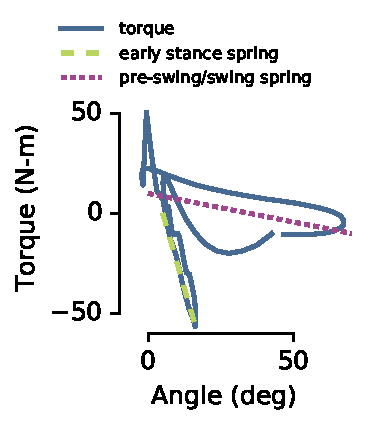
\includegraphics[width=\linewidth]{knee_torque_vs_angle}
    \caption{Torque vs angle relationship for the knee during level ground
    walking. Knee displays more complicated functionality than the ankle (see
    \cref{fig:ankle_torque_vs_angle}), with two distinct springs need to explain
    early stance and pre-swing/swing behavior. Data from
    \citet{winter2009biomechanics} scaled to 85 kg subject.}
    \label{fig:knee_torque_vs_angle}
\end{marginfigure}

The AAAKP prosthesis uses two unidirectional springs, one for extension and one
for flexion, each in series with its own actuator. With this setup,
AAAKP is able to store energy during the knee flexion phase just after heel
strike, and transfer it to a flexion spring for use during pre-swing and swing.
The prosthesis consumes just \unitfrac[5.6]{J}{stride}. However, the downside of
this design is inefficient use of actuator mass, as two electric motors are
required, one for extension and one for flexion.

A second concept is to use a series elastic actuator with a clutch on the motor
\citep{rouse2014clutchable, rouse2015design} The clutch saves energy by holding
the motor side of the series spring stationary while the spring is loaded in
early stance; no electrical energy is consumed holding the rotor in place. In
this design the spring-like behavior of the knee during swing is reproduced by
the electric motor alone unlike in the AAAKP prosthesis. Despite this, the
CSEA knee consumes less energy than the AAAKP, just \unitfrac[3.6]{J}{stride}.
Moreover, the simplified design of the CSEA has a mass of \unit[2.7]{kg} vs
\unit[3.6]{kg} for the AAAKP.

A potential drawback of SEA designs that are tuned for energy efficiency is that
they typically tune tune the spring stiffness to match observed quasi-stiffness
of the biological joint during a certain phase of the gait. However, this
stiffness value is not necessarily that which maximizes torque control
bandwidth. Therefore, while prostheses tuned for efficiency can consume less
energy, which is desirable for a product needing long battery life, they may
not represent the most versatile design for evaluating new control ideas or
different gait modes. 

\section{Stumble Recovery for Prostheses}\label{sec:back_stumble_recovery}
The prosthesis controls we reviewed in
\cref{sec:back_walking_review,sec:back_bioinspired_pros_control} primarily
sought to reproduce typical walking kinematics and dynamics. Some control
strategies, such as neuromuscular reflex control
(\cref{sec:back_neuromuscular_reflexes}) also demonstrated the ability to
generalize to sloped walking and changes in speed by producing more push off
work in these situations \citep{eilenberg2010control, markowitz2011speed}.
However, it is not clear that the low-level reflexes in the neuromuscular
control model will generate trip recovery responses, which in human control
likely utilize more complex supraspinal and cortical reflexes
\citep{eng1994strategies, schillings2000muscular, hofstad2009evidence}.
We therefore seek to improve upon neuromuscular control's inherent stability
by augmenting it with explicit trip detection and recovery actions.

As discussed in \cref{sec:intro_motivation}, falling and the fear of physical
activity it engenders are two major issues amputees face
\citep{miller2001prevalence}. Avoidance of physical activity can potentially
cause deterioration of strength, balance and control, which may lead to further
inactivity, debilitation, and social isolation. Currently, the microprocessor
controlled, mechanically-passive prostheses feature trip recovery modes
that ``lock'' or highly damp knee movement. However,
\citet{bellmann2010comparative} show that these modes fail to adequately respond
to trips during a large portion of swing due to knee buckling at touch-down.
Moreover, it is unclear that passive, locking responses are intuitive for
amputees or coordinate well with innate trip recovery responses, which can
require positive joint power \citep{cordero2005energy}. However, the advent of
active transfemoral prostheses give us the opportunity to replicate amputee's
preferred responses, which will hopefully yield more effective and intuitive
fall-prevention actions.

\subsection{Responses to Trips}

Able-bodied persons primarily use two strategies to recover from trips to their
swing legs: When the tripped in early swing, people usually use an
\emph{elevating strategy}, in which the knee is actively flexed to lift the foot
over and in front of the obstacle. In late swing, people typically use a
\emph{lowering strategy}, in which knee extensor muscles rapidly bring the foot
in contact with the ground in front of the obstacle \citep{eng1994strategies}.
In response to mid-swing trips, people may use either strategy
\citep{schillings2000muscular}. Finally, the \emph{delayed lowering} can also be
used in early swing. This strategy is an aborted attempt at an elevating
strategy, followed by a lowering strategy, and is used when the toe catches
on the obstacle \citep{eng1994strategies}.

Interestingly, \citet{shirota2015transfemoral} show that transfemoral amputees
using mechanically-passive prostheses utilize these same strategies despite the
lack of control and positive power production at the knee joint. Amputees
compensated for these deficiencies and achieved elevating, lowering, and delayed
lowering foot trajectories via movements of the hip and sound side leg. The lack
of sensory feedback information from the prosthesis leg to the nervous system
did not seem to impede utilization of these strategies.  Consequently, the
authors hypothesize that mimicking able-bodied responses to trips may also be
intuitive for amputee subjects. 

While amputees using mechanically-passive prostheses exploit the same strategies
as able-bodied subjects for trip recovery, they do not use these strategies in
the same proportions during the phases of swing as do able-bodied subjects.
Amputees typically use elevating strategies less frequently and lowering
strategies more frequently. This difference increases when the prosthesis is the
stance leg, and the intact leg is tripped. A possible reason for decreased
reliance on the elevating strategy may stem from the inability of
mechanically-passive prostheses to produce positive joint power.
\citet{cordero2005energy} show that in an elevating strategy, positive power is
required in the swing-leg's knee joint in order to rapidly flex the knee to
achieve obstacle clearance. Likewise, \citet{pijnappels2004contribution} show
that powered stance leg push-off helps raise the foot during the elevating
strategy. Empowering transfemoral prostheses with active joints may help
amputees more easily realize the elevating strategy, normalize amputee trip
recovery strategy selection, and allow them to recover from a larger range of
disturbances.

\subsection{Trip Detection and Classification}
Human responses to gait disturbances likely involve signal processing at the
supraspinal and cortical level. This is evidenced by the relatively high latency
($>\unit[100]{ms}$) of EMG signals relevant to the utilized strategy, the
utilization of both elevating and lowering strategies in mid-swing, the
existence of the delayed lowering strategy \citep{schillings2000muscular}, and
the inconsistent resolution of motor redundancy during the lowering strategy
\citep{eng1994strategies}. Furthermore, \citet{hofstad2009evidence} found that
latencies are further increased for amputee subjects executing obstacle
avoidance tasks, suggesting that amputee trip recovery may require additional
data processing and cognitive control as compared to able-bodied persons. 

A control system that seeks to be intuitive and effective for amputees by
mimicking their responses to trips needs to be able to model these complexities.
As a result, researchers have relied on data-driven and machine learning
approaches to detect and classify trips so that prostheses can take the
appropriate actions. All systems designed to date use a two-layer classification
scheme, where the first layer distinguishes trips from normal walking, and the
second layer classifies the recovery strategy as either elevating or lowering.
The first such system by \citet{lawson2010stumble} used Fast Fourier Transform
features of data collected from six accelerometers placed on the lower limb. To
collect training data, the author's outfitted healthy subjects with sensors, and
randomly subjected them to trips. They classified stumbles from normal walking
via a threshold on power between 10 and \unit[40]{Hz} and classified elevating
versus lowering strategies based on the root-mean-squared thigh acceleration in
a \unit[50]{ms} window before the stumble. \citet{zhang2011towards} further add
EMG sensors to the trip detection system, and employ outlier detection methods
so that the trips were not required in the training dataset. They find EMG sensors
improve the false alarm rate, at the expense of classification latency. However,
the false alarm rate is still quite high, corresponding to an incorrect positive
classification every \unit[1.6]{min}. Finally, \citet{shirota2014recovery} use
linear discriminant analysis on kinematic features from the tripped leg. They
find evidence supporting the use of the two-stage classification scheme, and
identify the optimal update frequency and length for the window in which they
compute features.

A major drawback of these previous works is that they report error rates based
on offline validation results; \ie they collect data from subjects who are
responding to trips and then evaluate how well the classifier would have
performed on the collected data. This is fundamentally different than online
validation, in which one reports the error rate obtained when using the
learned classifier to control the system. Previous work on a classifier for
recognizing gait modes such as level walking and stair and ramp ascent and
descent found that online error rates were significantly higher than offline
error rates \citep{hargrove2015intuitive}. As we discuss in
\cref{sec:proposed_trip_recovery}, it is likely this trend will hold true for
stumble classification as well.

\chapter{Neuromuscular Model}\label{sec:neuro_model}
\begin{marginfigure}
    \centering
    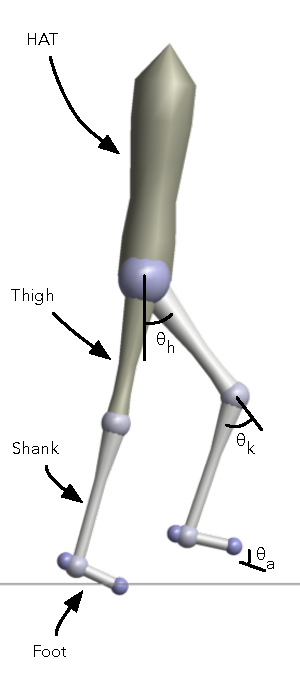
\includegraphics[width=\linewidth]{neuro_mech_model}
    \caption{The skeletal model we use to simulate neuromuscular reflex control.
    The model consists of seven segments: left and right feet, shanks, and
    thighs, as well as a lumped head-arms-trunk (HAT) segment. Flexion joint
    angles are positive, extension joint angles are negative, and the zero
    angle configuration represents standing.}
    \label{fig:neuro_seven_link}
\end{marginfigure}

In this thesis we intend to investigate the ability of neuromuscular reflex
control to improve amputee gait robustness. To this end, here we provide a more
detailed review the neuromuscular model components on which we base our
prosthesis control. Four parts comprise the model: a mechanical simulation
environment we use to obtain simulation results (\cref{sec:neuro_mech_model}),
biological motors modeled by the hill muscle model that apply torques to joints
(\cref{sec:neuro_hill_muscle}), and finally functionally-motivated stance
(\cref{sec:neuro_stance_reflexes}) and swing (\cref{sec:neuro_swing_reflexes})
reflexes that implement the key behaviors required for walking.

\section{Mechanical Model}\label{sec:neuro_mech_model}

To obtain the simulation results we present in \cref{sec:completed_comparison},
we construct a mechanical model in the Matlab Simscape Multibody environment
similar to those presented in \citet{geyer2010muscle, song2013integration,
song2015neural}.  This model represents the seven link biped in
\cref{fig:neuro_seven_link} and includes two legs with thigh, shank, and foot
segments as well as a lumped head-arms-trunk (HAT) segment.
\Cref{tab:model_mech_params} lists the segment lengths, center of mass and joint
locations measured from the distal end, masses, and inertias that approximate
those of a \unit[80]{kg}, \unit[2.0]{m} tall person.

\begin{table}[b]
  \centering
      \begin{tabular}{lllll}
        \toprule
        & Feet & Shanks & Thighs & HAT \\
        \midrule
        $l         \ (\unit{cm})$ & 20    & 50   & 50   & 80   \\
        $d_\tn{COM}   \ (\unit{cm})$ & 14    & 30   & 30   & 35   \\
        $d_\tn{Joint} \ (\unit{cm})$ & 16    & 50   & 50   &      \\
        $m         \ (\unit{kg})$ & 1.25  & 3.5  & 8.5  & 53.5 \\
        $J         \ (\unit{kg})$ & 0.005 & 0.05 & 0.15 & 3    \\
        \bottomrule
      \end{tabular}
  \caption{Segment lengths $(l_s)$, center of mass $(d_\tn{COM})$ and joint
  $(d_\tn{Joint})$ locations measured from the distal end, masses $(m)$, and
  inertias $(J)$ approximated from
  \citet{gunther2003synthesis}.}\label{tab:model_mech_params}
\end{table}

The mechanical model interacts with the environment through ground reaction
forces on the toes and balls of the feet. Specifically, we use a 2-dimensional
reduction of the 3D ground contact model presented in
\citet{song2013generalization} to calculate forces in the normal and
tangential directions with respect to the terrain. In the normal direction the
force is
\begin{align}
    F_\tn{n} = k_\tn{n} \Delta n_c (1 + \dot n_c) (\Delta n_c > 0)
    \left(\nicefrac{\dot n_c}{v_\tn{max}} > -1 \right),
    \label{eq:grf_n}
\end{align}
where $k_\tn{n} = \unitfrac[78.45]{N}{mm}$ is the stiffness coefficient in
the normal direction and $\Delta n_c$ and $\dot n_c$ are the normal penetration
in the normal direction and velocity. The form of the normal force is inspired
by \citet{gunther2003synthesis, scott1993biomechanical} and represents a linear
spring with multiplicitive damping.  $v_\tn{max} = \unitfrac[3]{cm}{s}$ represents
the maximum recovery velocity of the ground. If $\dot n_c$ exceeds this
velocity ground contact is lost.

In the tangential direction, a state machine switches between two force models
representing sliding and static friction. Sliding friction is given by
\begin{align}
    F_{\tn{t,slide}} = -\func{sign}{\dot t_c} \mu_\tn{slide} F_n
\end{align}
while static friction is given by
\begin{align}
    F_{\tn{t,static}} = -k_t \Delta t_c \left(1 + \func{sign}{\Delta t_c}
    \frac{\dot t_c}{v_\tn{max}} \right),
\end{align}
where $\Delta t_c$ is the penetration in the tangential direction $\dot t_c$ is
the penetration velocity, $\mu_\tn{slide} = 0.8$ is the sliding coefficient of
friction, and $k_\tn{t} =\unitfrac[78.45]{N}{mm}$ is the stiffness coefficient
in the tangential direction.

The contact model begins in the sliding mode and switches to the static mode if
$\dot t_c < 1 \unitfrac[1]{cm}{s}$. It switches back to the sliding mode when $|
F_{\tn{t,static}} | < \mu_\tn{static} | F_n |$, where $\mu_\tn{static} = 0.9$.

Finally, the biped skeletal model includes soft joint limits to represent
the skeletal joint limits on the knee, ankle, and hip joints. The functional
form form the soft limit joint torque is identical to that of the normal ground
reaction force given by \cref{eq:grf_n}.
\begin{align}
    \tau_{jl} = k_{jl} \Delta \phi_{jl} (1 + \dot \phi_{jl}) (\Delta
    \phi_{jl}  > 0) \left(\nicefrac{\dot \phi_{jl}}{\dot \phi_\tn{max}} > -1
    \right), 
    \label{eq:tau_joint_limit}
\end{align}
where $k_{jl} = \unitfrac[0.3]{N \cdot m}{deg}$ is the joint stiffness $\Delta
\phi$ and $\dot \phi_{jl}$ are the joint limit penetration angle and
velocity respectively, and $\dot \phi_\tn{max} = \unitfrac[1]{deg}{s}$ is the
maximum joint limit retraction velocity. \Cref{tab:joint_lim} lists the
engagement angles for the joint limits.
\begin{margintable}[-0.65in]
  \centering
      \begin{tabular}{lll}
        \toprule
        Joint & ext.\ lim.\ & flex lim.\ \\
        \midrule
        hip   &     & 50 \\
        knee  &   5 &    \\
        ankle & -40 & 20 \\
        \bottomrule
      \end{tabular}
  \caption{Joint limits for the hip, knee, and ankle joints listed in degrees.
  Positive joint angles represent flexion and negative joint angles represent
  extension (see \cref{fig:neuro_seven_link}).}\label{tab:joint_lim}
\end{margintable}

To obtain simulation results, we simulate the mechanical system with the ode15s
variable step solver. We set the maximum step size to \unit[10]{ms}, relative
error tolerance to $10^{-4}$, and abolute error to $10^{-6}$.

\section{Hill Muscle Models}\label{sec:neuro_hill_muscle}
\begin{marginfigure}[-0.25in]
    \centering
    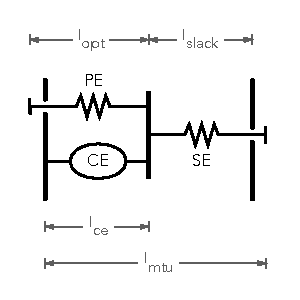
\includegraphics[width=\linewidth]{mtu_figure}
    \vspace{-0.4in}
    \caption{Hill-type muscle tendon unit with contractile element (CE),
    parallel elasticity (PE), and series elasticity (SE).}
    \label{fig:hill_type_mtu}
\end{marginfigure}
Our proposed transfemoral prosthesis control is comprised of biological muscle
actuators that are stimulated according to hypothesized reflex pathways.
Specifically, we use a Hill-type \emph{muscle tendon unit} (MTU) developed in
\citet{geyer2010muscle}. It is comprised of a contractile element (CE) that
represents muscle fibers and produces force when activated, a parallel elastic
(PE) element that represents the stiffness of the collagen tissue between muscle
fascicles, and series elastic (SE) element that models tendon stretch.
\Cref{fig:hill_type_mtu} shows the arrangement of these elements. Note that the
PE and SE both are unidirectional springs with engagement lengths of
$l_\tn{opt}$ and $l_\tn{slack}$ respectively.

The CE generates force according to
\begin{align}
    F_\tn{CE} = F_\tn{max} A \func{f_l}{l_\tn{CE}} \func{f_v}{v_\tn{CE}}.
    \label{eq:hill_ce}
\end{align}
In this equation, the force generated by the CE $(F_\tn{CE})$ is the maximum
isometric (constant length) force $(F_\tn{max})$ multiplied by activation $(A)$,
the force-length ($\func{f_l}{\cdot})$, and force-velocity
$(\func{f_v}{\cdot})$, relationships of the CE. The activation $A$ is a low-pass
filtered version of the stimulation signal muscle $S(t)$ generated by the muscle
reflexes we will detail in the \hyperref[sec:neuro_stance_reflexes]{next}
section. This filter, given by $A(t) = S - \tau \dot A(t)$ with time constant
$\tau$, represents the diffusion dynamics of calcium ions that activate binding
sites in the muscle fibers.
\begin{marginfigure}[-1in]
    \centering
    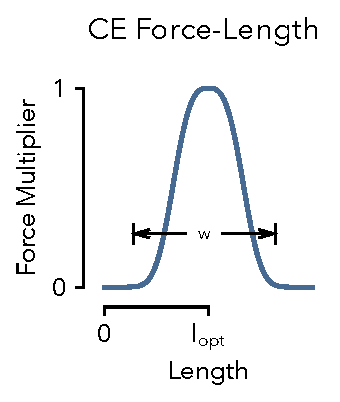
\includegraphics[width=\linewidth]{force_length_ce_annotate}
    \vspace{-0.25in}
    \caption{Force-length relationship of the CE.}
    \label{fig:force_length_ce}
\end{marginfigure}

The binding sites are where overlapping actin and myosin filaments attach and
generate pulling force. The contractile element length of $l_\tn{opt}$
corresponds to maximum overlap between these filaments. Therefore, as as the
muscle length moves away from $l_\tn{opt}$, its force production capacity
decreases leading to the force-length relationship shown in
\cref{fig:force_length_ce}. We model the force-length relationship via a bell
curve
\begin{align}
    \func{f_l}{l_\tn{CE}} = \exp \left( \ln(0.05) \left|
    \frac{l_\tn{CE} - l_\tn{opt}}{w l_\tn{opt}}
    \right|^3 \right).
    \label{eq:hill_force_length}
\end{align}
\begin{marginfigure}[0.25in]
    \centering
    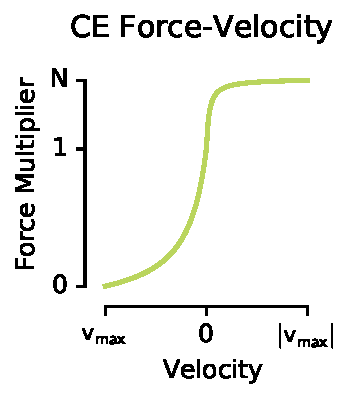
\includegraphics[width=\linewidth]{force_velocity_ce}
    \vspace{-0.25in}
    \caption{Force-velocity relationship of the CE.}
    \label{fig:force_velocity_ce}
\end{marginfigure}

The velocity-dependent filament attachment probabilities give rise to a
force-velocity relationship shown in \cref{fig:force_velocity_ce}. The following
expression captures this relationship.
\begin{table}[t]
  \centering
  \begin{tabular}{ll|ll}
    \toprule
    Param & Value             & Param                   & Value \\
    \midrule                           
    $\tau$ & \unit[0.1]{s}    & $l_\tn{opt}^\tn{ham}$   & \unit[0.10]{m} \\
    $w$    & 0.56             & $v_\tn{max}^\tn{ham}$   & \unitfrac[-1.2]{m}{s} \\
    $K$    & 5                & $F_\tn{max}^\tn{ham}$   & \unit[3000]{N} \\
    $N$    & 1.5              & $l_\tn{slack}^\tn{ham}$ & \unit[0.31]{m} \\
    $\epsilon_\tn{PE}$ & $w$  &                         & \\
    $\epsilon_\tn{SE}$ & 0.04 &                         & \\
    \bottomrule
  \end{tabular}
  \caption{Neuromuscular parameters for shared entities (left) and the hamstring
  muscle (right)}
  \label{tab:neuromusc_params}
\end{table}
\begin{align}
    \func{f_v}{v_\tn{CE}} = 
    \begin{cases} 
        \frac{v_\tn{max} - v_\tn{CE}}{v_\tn{max} + K v_\tn{CE}}, & \tn{if } v_\tn{CE}< 0 \\
        N + (N-1) \frac{v_\tn{max} + v_\tn{CE}}{7.56 K v_\tn{CE} - v_\tn{max}}, &
            \tn{if } v_\tn{CE} \ge 0 
    \end{cases}
\end{align}
In this expression, $K$ is a shape parameter and $N$ determines the force
amplification when the contractile element is lengthening. The force-velocity
relationship acts as a multiplicative damper causing the CE to produce more
contractile force when it is lengthening and less as it extends.

We model both passive elements, the PE and SE, using the same functional form
representing a unidirectional, stiffening spring, the behavior of which is shown
in \cref{fig:force_length_pese}. The expressions for the elastic force produces
by these elements are
\begin{align}
    \func{F_\tn{PE}}{l_\tn{CE}} &= F_\tn{max} \left( \frac{l_\tn{CE} - l_\tn{opt}}{\epsilon_\tn{PE}
        l_\tn{opt}} \right)^2 (l_\tn{CE} > l_\tn{opt})\\
    \func{F_\tn{SE}}{l_\tn{SE}} &= F_\tn{max} \left( \frac{l_\tn{SE} - l_\tn{slack}}{\epsilon_\tn{SE}
        l_\tn{slack}} \right)^2 (l_\tn{SE} > l_\tn{slack}).
\end{align}
\begin{marginfigure}
    \centering
    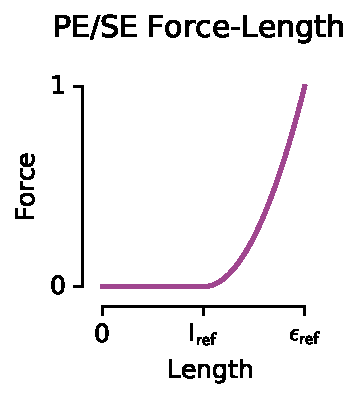
\includegraphics[width=\linewidth]{force_length_pese}
    \caption{PE and SE force length relationship. For the PE, $l_\tn{ref} = l_\tn{opt}$
    and $\epsilon_\tn{ref} = \epsilon_\tn{PE}$. Likewise, for the SE, $l_\tn{ref} =
    l_\tn{slack}$ and $\epsilon_\tn{ref} = \epsilon_\tn{SE}$.} 
    \label{fig:force_length_pese}
\end{marginfigure}

The left-hand side of \cref{tab:neuromusc_params} lists the parameters common
among all seven muscles of each leg of the neuromuscular model. On the
right-hand side of the table, we list four muscle-specific parameters for
hamstrings muscle. For a complete list of muscle parameters please refer
to \citet{song2015neural}. 

\begin{figure}[b]
    \centering
    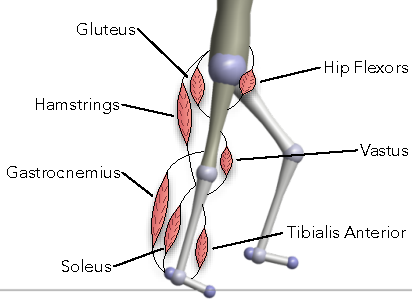
\includegraphics[width=3in]{biped_w_muscles}
    \caption{Biped walking model with labeled muscles.} 
    \label{fig:biped_w_muscles}
\end{figure} 
The full biped model, shown in \cref{fig:biped_w_muscles}, includes
seven Hill-Type muscle-tendon units: soleus, gastrocnemius, tibialis anterior,
vastus, hamstring, hip flexors, and gluteus. The length of these MTUs is related
to the joint angles according to the variable-length moment arms
$\func{r_}[\tn{mtu}][j]{\phi^j}$ for each muscle about each joint. For example,
the length of a biarticular muscle spanning joints $j$ and $k$ is
\begin{align}
    l_\tn{mtu} = l_\tn{opt} + l_\tn{slack} + \rho \left( \int_{\phi_0^j}^{\phi^j}
        \func{r}[\tn{mtu}][j]{\phi^j} \tn{d} \phi^j + \int_{\phi_0^k}^{\phi^k}
        \func{r}[\tn{mtu}][k]{\phi^k} \tn{d} \phi^k \right).
\end{align}
Where $\rho$ is a parameter that approximates the effect of the pennation angle 
of the muscle fibers. The variable length moment arms also govern the torque a
muscle produces about a joint according to
\begin{align}
    \tau_\tn{mtu} = \func{r}[\tn{mtu}][j]{\phi^j} F_\tn{mtu}.
\end{align}

\section{Stance Reflexes}\label{sec:neuro_stance_reflexes}

During stance, hypothesized reflex feedback pathways stimulate the muscles of
the leg. In general, a linear feedback law governs the stimulation
$\func{S}[][m]{t}$ of muscle $m$, 
\begin{align}
    \func{S}[][m]{t} = S_0^m + \sum_n G_n^m \func{Pro}[n][]{t - \Delta t_n},
\end{align}
where $S_0^m$ is a constant pre-stimulation, $\func{Pro}[n][]{t - \Delta t_n}$
is the time-delayed proprioceptive signal from muscle $n$, and $G_n^m$ is the
gain on that signal. The proprioceptive signal can take the form of force
feedback, $\func{F}[\tn{n}][m]{\cdot}$, which uses the time delayed tendon
force, or length feedback, $\func{L}[\tn{n}][m]{\cdot} =
\func{l}[\tn{CE},n][]{\cdot} - l_{\tn{off}, n}$, which uses the difference
between the length of the contractile element and an offset length
$l_n^\tn{off}$.

The time delay we apply to proprioceptive signals estimate the round-trip neural
signal transmission delay of afferent signals from muscle spindles and Golgi
tendons to the spine and efferent signals back to the muscles. For ankle
muscles, the soleus, tibialis anterior, and gastrocnemius, the time delay is
$\Delta t_n = \unit[20]{ms}$. For knee muscles, the vastus and hamstrings, it is
$\Delta t_n = \unit[10]{ms}$. For the hip muscles, the hamstrings, gluteus, and
hip flexors, the time delay is $\Delta t_n = \unit[5]{ms}$. We will denote time
delayed signals using $t_\tn{l} = t - \unit[20]{ms}$, $t_\tn{m} = t -
\unit[10]{ms}$, and $t_\tn{s} = t - \unit[5]{ms}$.


The reflexes encode several key functions of legged locomotion: generating
compliant leg behavior, preventing knee overextension, and balancing the trunk.

The reflexes achieve the first function, generating compliant leg behavior, via
positive force feedback on the monoarticular leg extensors: the soleus, vastus,
and gluteus. For example, the reflexes stimulated the vastus in part by
\begin{align}
    \func{S}[][\tn{vas}]{t} = S_0^\tn{vas} + 
        G_\tn{vas}^\tn{vas} \func{F}[\tn{vas}][]{t_\tn{m}} + \ldots \:.
\end{align}

To implement the second function, preventing knee overextension, the reflex
control uses two strategies. First, positive force feedback of the biarticular
gastrocnemius and hamstrings muscles helps counteract the tendency for knee
overextension caused by ankle plantarflexion and hip extension torques,
respectively. For example, the gastrocnemius has a force feedback reflex,
\begin{align}
    \func{S}[][\tn{gas}]{t} = S_0^\tn{gas} + 
        G_\tn{gas}^\tn{gas} \func{F}[\tn{gas}][]{t_\tn{l}} \:,
        \label{eq:gas_stim}
\end{align}
that flexes the knee as it contributes to anklep plantarflexion. The hamstring
also has a positive force feed back
\begin{align}
    \func{S}[][\tn{ham}]{t} = S_0^\tn{ham} + 
        G_\tn{ham}^\tn{ham} \func{F}[\tn{ham}][]{t_\tn{s}} + \ldots \:
        \label{eq:ham_stim}
\end{align}
that counteracts knee flexion caused by hip extension. Also, the hamstring force
feedback helps prevent hip flexion caused by heel-strike.

A second mechanism further protects the knee by inhibiting the vastus
stimulation in proportion to knee extension beyond a threshold, resulting in
the complete vastus stimulation
\begin{align}
    \func{S}[][\tn{vas}]{t} &= S_0^\tn{vas} + 
        G_\tn{vas}^\tn{vas} \func{F}[\tn{vas}][]{t_\tn{m}} 
            -k_\phi \left(\phi_\tn{k}(t_\tn{m}) - \phi_\tn{k}^\tn{off} \right)
            \notag \\
        &\quad \times 
            \left( \phi_\tn{k}(t_\tn{m}) < \phi_\tn{k}^\tn{off} \right)
            \left( \dot \phi_\tn{k}(t_\tn{m}) < 0\right) \label{eq:vas_stim_full} 
\end{align}
where $\phi_\tn{k}^\tn{off}$ is the angle beyond which the vastus is inhibited.

The reflexes achieve the final function of balancing the trunk by
proportional-derivative control that produces stimulations for the hip muscles
(hip flexors, gluteus, and hamstrings) to stabilize the trunk at a reference
lean. Because muscles can only provide pulling force, the proportional derivative
control signal is distributed as hip flexor stimulation if the signal represents
flexion torque and as simultaneous stimulation for the gluteus and hamstrings if
it represents hip extension torque. For example, the complete hamstrings
stimulation becomes
\begin{align}
    \func{S}[][\tn{ham}]{t} &= S_0^\tn{ham} + 
        G_\tn{ham}^\tn{ham} \func{F}[\tn{ham}][]{t_\tn{s}} \notag\\
            &\quad +  \left\{ k_\tn{p}^\tn{ham} 
            (\phi_\tn{trunk}(t_\tn{s}) - \phi_{\tn{ref}}) 
            + k_\tn{d}^\tn{ham} \dot{\phi}_{\tn{trunk}}(t_\tn{s}) \right\}_+ 
        \label{eq:ham_stim_full}
\end{align}
where the third term returns the positive reflex contribution from the trunk
balance control. 

\begin{fullwidth}
The full set of stance reflexes are:
\begin{align}    
    \func{S}[][\tn{sol}]{t} &= S_0^\tn{sol} + 
        G_\tn{sol}^\tn{sol} \func{F}[\tn{sol}][]{t_\tn{l}} \\
    \func{S}[][\tn{ta}]{t} &= S_0^\tn{ta} + 
        G_\tn{ta}^\tn{ta} \func{L}[\tn{ta}][]{t_\tn{l}} - G_\tn{sol}^\tn{ta} 
        \func{F}[\tn{sol}][]{t_\tn{l}}\\
    \func{S}[][\tn{gas}]{t} &= S_0^\tn{gas} + 
        G_\tn{gas}^\tn{gas} \func{F}[\tn{gas}][]{t_\tn{l}} \\
    \func{S}[][\tn{vas}]{t} &= S_0^\tn{vas} + 
        G_\tn{vas}^\tn{vas} \func{F}[\tn{vas}][]{t_\tn{m}} 
        -k_\phi \left( \phi_\tn{k}(t_\tn{m}) - \phi_\tn{k}^\tn{off} \right) 
        \left( \phi_\tn{k}(t_\tn{m}) < \phi_\tn{k}^\tn{off} \right)
        \left( \dot \phi_\tn{k}(t_\tn{m}) < 0\right) \\     
    \func{S}[][\tn{ham}]{t} &= S_0^\tn{ham} + 
        G_\tn{ham}^\tn{ham} \func{F}[\tn{ham}][]{t_{s}} 
        + \left\{ k_\tn{p}^\tn{ham} (\phi_{\tn{trunk}} - \phi_{\tn{ref}}) 
        + k_\tn{d}^\tn{ham} \dot{\phi}_{\tn{trunk}} \right\}_+ \\
    \func{S}[][\tn{glu}]{t} &= S_0^\tn{glu} + 
        G_\tn{glu}^\tn{glu} \func{F}[\tn{glu}][]{t_{s}}
        + \left\{ k_\tn{p}^\tn{glu} (\phi_{\tn{trunk}} - \phi_{\tn{ref}}) 
        + k_\tn{d}^\tn{glu} \dot{\phi}_{\tn{trunk}} \right\}_-  \\
    \func{S}[][\tn{hfl}]{t} &= S_0^\tn{hfl} + 
        \left\{ k_\tn{p}^\tn{hfl} (\phi_{\tn{trunk}} - \phi_{\tn{ref}}) 
        + k_\tn{d}^\tn{hfl} \dot{\phi}_{\tn{trunk}} \right\}_+ 
\end{align}    
\end{fullwidth}

\section{Swing Leg Control}\label{sec:neuro_swing_reflexes} During swing, the
reflexes shape the natural double pendulum dynamics of the leg in order to
achieve sufficient knee flexion, prevent toe scuffing, reach a target landing
leg angle, and then extend the leg towards the ground. We here review two
versions of the swing leg control: First, an idealized control, proposed in
\citet{desai2012robust}, which proposes reflexes that directly applies torques
to the hip and knee joints (\cref{sec:neuro_ideal_swing}), and second, a muscle
reflex control, presented in \citet{desai2013muscle}, which applies neural
stimulations to Hill-type muscles to achieve the functionality of the idealized
control (\cref{sec:neuro_muscle_swing}).

\subsection{Idealized Swing Leg Control}\label{sec:neuro_ideal_swing}
The idealized swing control comprises two layers. In the first layer, a leg
placement policy,
\begin{align}
    \alpha_{\tn{tgt}} = \alpha_{0} + c_\tn{d} d + c_\tn{v} v,
    \label{eq:simbicon}
\end{align}
prescribes leg angle for the leg to reach by the end of swing. We measure the
leg angle between the hip-ankle line and horizontal as shown in
\cref{fig:swing_leg_polar}. In \cref{eq:simbicon}, $\alpha_{\tn{tgt}}$ is the
target leg angle, $\alpha_{0}$ is the default leg angle, $d$ is the horizontal
distance between the stance leg ankle and the model's center of mass, $v$ is the
velocity of the center of mass, and $c_\tn{d}$ and $c_\tn{v}$ are constant gain
parameters. This policy is taken from~\citet{yin2007simbicon} and represents an
empirical generalization of the leg placement strategies that recover the linear
inverted pendulum model of human walking from
disturbances~\citep{kajita20013d,pratt2006capture}. 

The target angle generated by this policy forms a central input to the second
layer comprised of hip and knee controls. The portion of this control that
governs the knee action uses a finite state machine to switch between three
phases. The first phase allows the knee to passively flex in response to hip
moments generated at the onset of swing. If the passive knee flexion is
insufficient (the foot swings forward with a tendency to scuff the ground), the
control produces active flexion torque of the knee in proportion to the rate
$\dot{\alpha}$ of forward leg motion,
\begin{marginfigure}
    \centering
    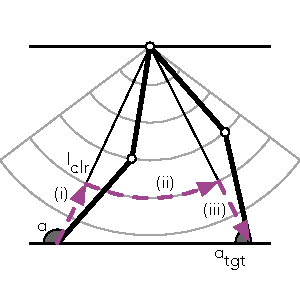
\includegraphics[width=\linewidth]{swing_leg_polar}
    \caption{The swing leg control guides the leg towards a desired landing leg
    angle $\alpha_\tn{tgt}$ through three phases: (i) Flex the knee until it
    achieves a clearance leg length $l_\tn{clr}$. (ii) Hold the leg length via
    knee damping. (iii) Stop and Extend the leg towards the ground when the leg
    reaches $\alpha_\tn{tgt}$. Figure reproduced from \citet{desai2012robust}.}
    \label{fig:swing_leg_polar}
\end{marginfigure}
\begin{align}
    \tau_\tn{k}^\tn{i} = \begin{cases}
                 0,                     & \dot{\alpha} > 0 \\
                -k^\tn{i} \dot{\alpha}, & \dot{\alpha} \le 0 
                \end{cases},
    \label{eq:flexphase}
\end{align}
where $k^\tn{i}$ is the flexion gain and the leg angle $\alpha$ is defined as
the angle between the horizontal and the hip-ankle line.  

The second phase activates when the leg length, defined as the distance between
the hip and ankle, contracts below a threshold. In this phase, the knee torque
is given by
\begin{align}
    \tau_\tn{k}^\tn{ii} = \begin{cases}
          -k_1^\tn{ii} \dot \phi_\tn{k}, & \dot \phi_\tn{k} \ge 0 \\
          -k_2^\tn{ii} \dot \phi_\tn{k}(\alpha - \alpha_\tn{tgt})
            (\dot{\alpha} - \dot \phi_\tn{k}), 
          & \dot\phi_\tn{k} < 0 \ \& \ \dot \phi_\tn{k} < \dot \alpha\\
          0, & \mathrm{otherwise}
      \end{cases},
    \label{eq:holdphase}
\end{align}
where $k_1^\tn{ii}$ and $k_2^\tn{ii}$ are damping coefficients. The first case
dampens knee flexion, while the second case dampens knee extension, but allows
progressively more extension as the leg angle approaches its target. The
modulation term $(\dot \alpha - \dot \phi_\tn{k})$ prevents premature landing of
the leg by damping the knee if it extends faster than the overall leg angle.

The third phase engages when the leg angle gets within a threshold of the
target leg angle. The control then applies torque to stop and extend the knee,  
\begin{align}
    \tau_k^\tn{iii} = 
    \begin{cases}
         k^\tn{iii}(\alpha_{\tn{thr}} - \alpha)
            \left(1 - \frac{\dot\alpha}{\dot\alpha_\tn{max}} \right), 
                & \alpha < \alpha_\tn{thr} \ \& \ \dot \alpha < \dot \alpha_\tn{max} \\
        0, & \tn{otherwise}
    \end{cases},
    \label{eq:stop}
\end{align}
where $\dot{\alpha}_{\mathrm{max}}$ is the maximum leg retraction velocity for
which the stopping knee torque is applied. When this torque brings the leg
velocity to zero, a knee extension torque is added,
\begin{align}
    \tau_\tn{k}^\tn{iii'} = \tau_\tn{k}^\tn{iii} - k^\tn{ext} (l_0 - l),
    \label{eq:extend}
\end{align}
where $l_0$ is the rest leg length, $l$ is the current leg length, and
$k^\tn{ext}$ is a proportional gain. 

The swing leg control also specifies a hip torque in the form of a proportional
derivative control on the leg angle, 
\begin{align}
    \tau_\tn{h}^\alpha = k_\tn{p} (\alpha - \alpha_\tn{tgt}) + k_\tn{d} \dot\alpha.
    \label{eq:hipfeedback}
\end{align}
This hip torque is supplemented by a feed forward term 
\begin{align}
    \tau_\tn{h} = \tau_\tn{h}^\alpha - 2 \tau_\tn{k}^\tn{iii}
    \label{eq:hipfeedforward}
\end{align} 
that neutralizes the coupling dynamics between the knee and hip during the
knee's stop and extend phase (Eq.~\ref{eq:stop}).

The torques produced by the swing controller augment the net torques produced by
the Hill-type muscles and reflexes during stance. At heel strike, the control
policy switches from using the swing leg control torques to the stance torques
generated by the muscle models. In late stance, the policy mixes the torques
specified by the stance and swing controllers by scaling the stance and swing
torques and muscle stimulations in proportion to the normalized ground reaction
force,
\begin{align}
    \tau_\tn{late stance} &= \tau_\tn{stance}(GRF) +
    \tau_\tn{swing}(1 - GRF),\\ 
    S^\tn{m}_\textrm{late stance}  &= S^\tn{m}(GRF).
\end{align}
During swing, only the swing leg torques are used.

\subsection{Neuromuscular Reflex Swing Leg Control}\label{sec:neuro_muscle_swing}
\begin{marginfigure}
    \centering
    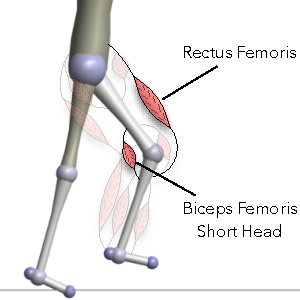
\includegraphics[width=\linewidth]{biped_w_muscles_rf_bfsh}
    \caption{Neuromuscular Swing leg control employs the seven muscles used in
    the stance control as well as a monoarticular knee flexor, the biceps
    femoris short head, and a biarticular hip flexor/knee extensor, the rectus
    femoris} 
    \label{fig:biped_w_muscles_rf_bfsh}
\end{marginfigure} 

The muscle reflex interpretation of the idealized swing leg control presented in
the previous \crefname{sec:neuro_ideal_swing} proposes reflexes to achieve the 
same three goals as the ideal swing leg control: (i) flex the knee to achieve
sufficient ground clearance, (ii) prevent toe scuffing by damping the knee (iii)
stop and extend the leg when the target leg angle is achieved (see
\cref{fig:swing_leg_polar}). This control assumes a leg with nine-muscles, the
seven included in the stance control (\cref{fig:biped_w_muscles}), as well as
two additional muscles shown in figure (\cref{fig:biped_w_muscles_rf_bfsh}).
These muscles are a monoarticular knee flexor, the biceps femoris short head,
and a biarticular hip flexor/knee extensor, the rectus femoris. As in the case
of the stance control, the reflexes primarily consist of linear feedback laws of
the form
\begin{align}
    \func{S}[phase][m]{t} = G_n^m \func{Pro}[n][]{t - \Delta t_n}.
\end{align}
For the swing control, the proprioceptive feedback can be either on length,
$\func{L}[n][m]{\cdot} = \func{l}[\tn{CE},n][]{\cdot} - l_{\tn{off}, n}$,
or velocity, $\func{V}[n][m]{\cdot} = \func{v}[\tn{CE},n][]{\cdot} -
v_{\tn{off}, n}$. In these equations $l_{\tn{off},n}$ and $v_{\tn{off}, n}$ are
offset lengths and velocities the control tries to obtain.

As in the idealized control, the knee control is divided into three phases. In
phase 1, the behavior of the idealized control is to provide knee flexion torque
in proportion to the rate of forward leg angle progression
(\cref{eq:flexphase}). The muscle interpretation uses the rate of length change
of the rectus femoris contractile element as a proxy for the speed of the leg
angle. It therefore implements phase 1 by stimulating a monoarticular knee
flexor, the biceps femoris short head, based on velocity feedback from the
rectus femoris.
\begin{align}
    \func{S}[i][\tn{bfsh}]{t} = G_\tn{rf}^\tn{bfsh}\func{V}[\tn{rf}][]{t_\tn{m}}.
\end{align}

In the second phase, the control dampens knee flexion and modulates the damping
of knee extension (\cref{eq:holdphase}, allowing more extension as the target
angle is approached and only damping the knee if it extends faster than the leg
angle progresses. In this phase, the control uses velocity feedback to dampen
knee flexion according to
\begin{align}
    \func{S}[\tn{ii}][\tn{rf}]{t} = G_\tn{bfsh}^\tn{bfsh}
        \func{V}[\tn{bfsh}][]{t_\tn{m}},
\end{align}
and a modified velocity feedback to dampen knee extension according to
\begin{align}
    \func{S}[\tn{ii}][\tn{bfsh}]{t} = G_\tn{bfsh}^\tn{bfsh}
        \func{V}[\tn{bfsh}]{t_\tn{m}} \func{L}[\tn{rf}][\tn{bfsh}]{t_\tn{m}} 
        \left( \func{V}[\tn{bfsh}]{t_\tn{m}} + \func{V}[\tn{rf}]{t_\tn{m}}
        \right).
\end{align}

The final task of the swing control, is to stop and extend the leg. Stopping is
achieved by length feedback on the hamstring
\begin{align}
    \func{S}[\tn{iii}][\tn{ham}]{t} = G_\tn{ham}^\tn{ham}
        \func{L}[\tn{ham}]{t_\tn{s}},
\end{align}
and is augmented by the other knee flexors if $\func{S}[\tn{iii}][\tn{ham}]{t} >
S_\tn{thr}$, where $S_\tn{thr}$ is a threshold.
\begin{align}
    \func{S}[\tn{iii}][\tn{bfsh}]{t} &= G_\tn{bfsh}^\tn{ham}
        \left (\func{S}[\tn{iii}][\tn{ham}]{t} - S_\tn{thr} \right) \\
    \func{S}[\tn{iii}][\tn{gas}]{t} &= G_\tn{gas}^\tn{ham}
        \left (\func{S}[\tn{iii}][\tn{ham}]{t} - S_\tn{thr} \right)
\end{align}
The control triggers knee extension through vastus length feedback, when the leg angle velocity crosses zero,
\begin{align}
    \func{S}[\tn{iii}][\tn{vas}]{t} = G_\tn{vas}^\tn{vas}
        \func{L}[\tn{vas}]{t_\tn{s}}.
\end{align}

The hip and ankle joints are controlled via length feedbacks. The hip control
approximates $\alpha$ through the length of the rectus femoris. Consequently,
the hip control uses length feedback from the rectus femoris in order to drive
the leg towards $\alpha_\tn{tgt}$,
\begin{align}
    \func{S}[][\tn{hfl}]{t} = S_0^\tn{hfl} + G_\tn{rf}^\tn{hfl}
        \func{L}[\tn{rf}]{t_\tn{s}} \\
    \func{S}[][\tn{glu}]{t} = S_0^\tn{glu} + G_\tn{rf}^\tn{glu}
        \func{L}[\tn{rf}]{t_\tn{s}}.
\end{align}
During swing length feedback on the tibialis anterior dorsiflexes the ankle to
prevent toe scuffing
\begin{align}
    \func{S}[][\tn{ta}]{t} = S_0^\tn{ta} + G_\tn{ta}^\tn{ta}
        \func{L}[\tn{ta}]{t_\tn{l}}
\end{align}

\chapter{Completed Work}\label{sec:completed_work}

\section{Transfemoral Prosthesis Design}\label{sec:completed_design}
\begin{marginfigure}[1.25in]
    \centering
    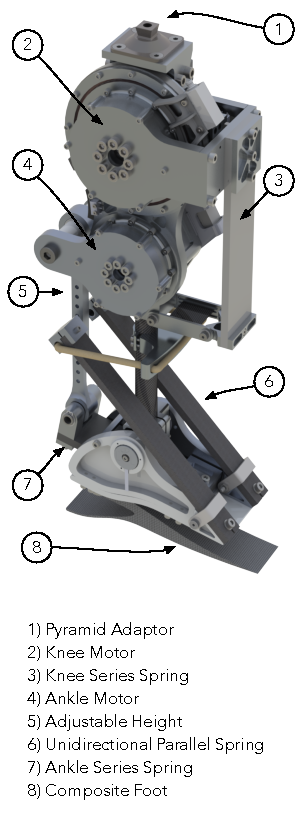
\includegraphics[width=\linewidth]{prosthesis_render_annotated}
    \caption{Render of proposed powered knee and ankle prosthesis design. The
    prosthesis includes series elastic actuators to enable accurate torque
    control and a unidirectional parallel ankle spring to offset the required
    angle torque.}\label{fig:prosthesis_render_annotated}
\end{marginfigure} 

\newthought{To test our proposed Neuromuscular control approach}, and its
ability to help subjects maintain or recover their balance, we build a custom
transfemoral prosthesis capable of reproducing dynamic locomotion tasks. The
proposed design, shown in \cref{fig:prosthesis_render_annotated}, uses brushless
electric motors coupled to harmonic drive gear sets to drive both the knee and
ankle joints.  Additionally, the joints employ series elastic actuation to
enable accurate torque control and to protect the prosthesis' gear sets from
sudden impacts.  The design also features a unidirectional parallel spring in
the ankle that partly offsets the torque demands on the ankle motor.  We design
both joints to meet the demands of dynamic locomotion tasks such as running and
trip recovery.

The overall design concept sits in a niche between low powered prostheses
designed with commercial applicability in mind
\citep{sup2007design,sup2009preliminary,lawson2014robotic,rouse2015design,
martinez2011antagonistic} which feature onboard actuation and power sources, and
high-powered tethered systems \citep{caputo2013experimental,
caputo2015informing} with off-board actuation designed exclusively for use in
lab environment. Our design features onboard actuators that are more powerful
than those used in standalone devices, but less capable than those employed in
tethered devices. To ensure a reasonable overall weight the device's batteries,
motor drivers, and computers are off-board. With this design, we expect to be
able to test control ideas without encountering hardware performance limitations
as with a tethered device. At the same time the device is capable of functioning
outside of the lab environment like a standalone prosthesis. 

\begin{table}
    \centering
    \begin{tabular}{lcc}
        \toprule
        Specification         & Desired Value & Achieved Value \\
        \midrule                  
        Maximum Knee Torque   & $\unit[160]{N \cdot m}$ 
            & $\unit[170]{N \cdot m}$   \\
        Maximum Knee Speed    & \unitfrac[1.80]{rev}{s} 
            & \unitfrac[1.93]{rev}{sec} \\
        Maximum Ankle Torque  & $\unit[200]{N \cdot m}$ 
            & $\unit[170 \ (+120^*)]{N \cdot m}$ \\
        Maximum Ankle Speed   & \unitfrac[1.14]{rev}{s} 
            & \unitfrac[1.22]{rev}{s} \\
        Weight                & \unit[6.8]{kg} & \unit[5.9]{kg} \\
        Minimum Height        & \unit[42.5]{cm} & \unit[42]{cm} \\
        \bottomrule
    \end{tabular}
    \caption{Designed and achieved design specifications. ($^*$Maximum total
    ankle torque is $\unit[290]{N \cdot m}$ achieved at \unit[10]{degrees} of
    dorsiflexion.)}\label{tab:pros_requirements}
\end{table}

\Cref{tab:pros_requirements} shows the desired design specifications for the
transfemoral prosthesis and the values achieved by the final design. To obtain
these design specifications we examined a number of studies that elicited trip
responses.

We specify desired joint torque and speed values to meet the requirements of
demanding tasks such as running. The maximum knee torque specification comes
from the findings of \citet{whitley2008maximum}, who tested the joint torques
used during recovery from a simulated fall. The maximum knee speed requirement
comes from \citet{grabiner1993kinematics}, who tested subjects' responses to
simulated trips induced by unseen obstacles on a walkway. We obtain the maximum
ankle torque requirement from \citet{pijnappels2005early}, who tripped subjects
using a obstacles that could suddenly emerge through the floor. The maximum
ankle speed requirement comes from the running data of
\citet{novacheck1998biomechanics}. We set to the minimum height specification,
measured between the center of the knee and bottom of the foot, to accommodate
the $10^\tn{th}$ percentile female \citep{gordon1988anthropometric}.  Finally,
the required weight corresponds to the mean leg weight of a $50^\tn{th}$
percentile male \citep{winter2009biomechanics}.

\subsection{Knee Joint}

In addition to achieving the maximum speeds and torques found in
\cref{tab:pros_requirements}, we design the knee joint so that it can reproduce
the torque and speed required for a \unit[80]{kg} person to run at
\unitfrac[3.2]{m}{s} as measured by \citet{novacheck1998biomechanics}. To
reproduce this trajectory in the knee joint, we utilize a RoboDrive ILM
$85\times13$ HS-SP motor coupled to a Harmonic Drive Gear set with a 50:1
reduction (CSG--25--50). \Cref{fig:knee_motor_torque} shows the motor torque
and speed required to reproduce a running trajectory assuming a gear
efficiency of $75\%$. In this plot, we see that the running trajectory lies
within the speed-dependent torque limit of the motor. Moreover, the root mean
squared torque of this trajectory $(\unit[1.46]{N \cdot m})$ exceeds the torque
rating of the motor $(\unit[1.43]{N \cdot m})$ by just $2\%$. Therefore, the
knee joint should be able to provide the necessary torque to enable running for
a short amount of time, or continuously for lighter subjects or at a slightly
reduced speed.
\begin{marginfigure}[-2in]
    \centering 
    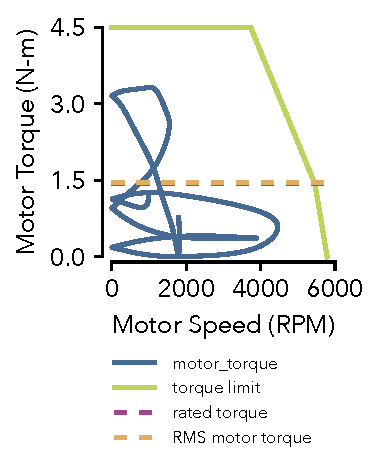
\includegraphics[width=\linewidth]{knee_motor_torque}
    \caption{Knee motor torque required for
    running}\label{fig:knee_motor_torque}
\end{marginfigure}

\begin{figure*}[t]
    \centering 
    \includegraphics[width=\linewidth]{knee_design}
    \caption{Internal and external design of the knee 
    joint.}\label{fig:knee_design}
\end{figure*}
\Cref{fig:knee_design} shows the internal and external design of the knee joint.
The primary component in the knee joint is the stator housing. On top of the
housing is a standard pyramid adaptor that allows the prosthesis to connect to
amputee's sockets. Within the stator housing, lies the brushless motor stator,
rotor, and harmonic drive gear set. We sense absolute rotor angle for
commutation of the brushless motor via hall effect sensors and a magnetic
complementary sin/cos encoder. To incorporate series elasticity, we take
inspiration from the design of the bipedal robot Atrias
\citep{grimes2013atrias}, which uses fiberglass series leaf springs. In our
design, the output of the gear set drives the proximal end of a fiberglass leaf
spring in series with the shank. Two Renishaw Resolute absolute encoders measure
the deflection of this spring to enable torque control.

\begin{marginfigure}[2.5in]
    \centering 
    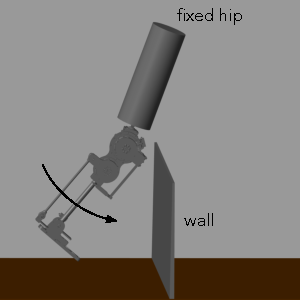
\includegraphics[width=\linewidth]{knee_impact_sim}
    \caption{Impact simulation we used to determine appropriate series spring
    stiffness.}\label{fig:knee_impact_sim}
\end{marginfigure}
In addition to allowing for accurate torque control, as shown by
\citet{au2007biomechanical,au2008powered}, the series elasticity also plays a
crucial role in protecting fragile gear components from impact loads. To choose
the spring stiffness for the knee joint, we simulate the prosthesis impacting a
rigid wall with the foot during swing. To do this, we construct a model of the
prosthesis in Matlab Simulink Simscape Multibody that includes the
series elasticity, gear dynamics, and motor electrical dynamics.
\Cref{fig:knee_impact_sim} shows the simulation environment. The prosthesis is
attached to the distal end of a thigh segment with a fixed hip position. We
control the hip via the ideal swing leg control outlined in
\cref{sec:neuro_ideal_swing} (\cref{eq:hipfeedback}) and consider the case where
the external voltage applied to the motor is zero. This simulation suggests that
a spring stiffness under $\unitfrac[2300]{N \cdot m}{rad}$ will ensure that the
peak impact torque remains lower than the peak allowable impact torque of the
Harmonic Drive of $\unit[242]{N \cdot m}$.

\subsection{Ankle Joint}
In the ankle joint we utilize a RoboDrive ILM $70\times10$ HS-SP motor coupled
to a Harmonic Drive Gear set with a 100:1 reduction (CSG--20--100). As with the
knee joint, we design the ankle joint to satisfy the requirements listed in
\cref{tab:pros_requirements}. Specifically, for the ankle joint we pay
considerable attention to the tripping condition described by
\citet{pijnappels2005early}, in which the ankle generates a peak torque of
$\unit[202]{N \cdot m}$. 

\begin{marginfigure}[-0in]
    \centering 
    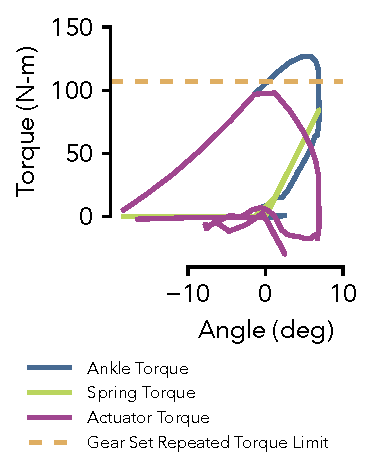
\includegraphics[width=\linewidth]{ankle_torque_vs_angle_ups}
    \caption{Ankle torque vs angle curve during steady, level-ground walking
    (blue) (\citet{winter2009biomechanics} scaled to \unit[80]{kg} person). A
    unidirectional parallel spring can provide a portion of this torque (green)
    and reduces the required actuator torque (purple) to lie under repeated
    torque limit of the Harmonic Drive Gear set (orange).
    }\label{fig:ankle_torque_vs_angle_ups}
\end{marginfigure}
To avoid using a large and heavy motor to achieve this peak torque, we take
inspiration from previous prosthetic ankle designs that employ a unidirectional
parallel spring in the ankle joint that performs the conservative portion of the
ankle's torque versus angle trajectory during normal walking
\citep{au2007biomechanical,au2008powered,sup2009preliminary,lawson2014robotic}.
The parallel spring offsets the required motor torque, as the actuator only
needs to provide the difference between the desired torque and the torque
provided by the parallel spring. \Cref{fig:ankle_torque_vs_angle_ups} shows the
torque versus angle curve during level ground walking
(\citet{winter2009biomechanics}, scaled to \unit[80]{kg} person). In green we
show the torque generated by a $\unitfrac[700]{N \cdot m}{rad}$ parallel spring
optimized to minimize the root-mean-squared motor torque for this trajectory.
From this plot, we see that with the parallel spring, the peak torque is lower
than the repeated peak torque limit of the Harmonic Drive Gear set.
\begin{figure}[b]
    \centering 
    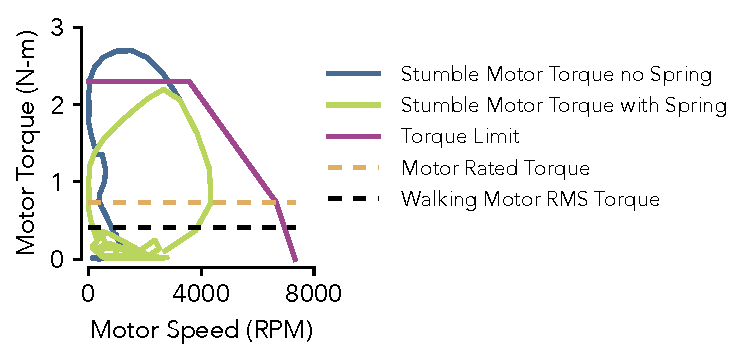
\includegraphics[height=2in]{ankle_motor_torque_tripping}
    \caption{Ankle motor torque required to take the trip recovery action
    observed by \citet{pijnappels2005early} (blue, trajectory obtained by
    scaling walking data from \citet{winter2009biomechanics} to a peak torque of
    $\unit[202]{N \cdot m}$, $75\%$ gear efficiency assumed). Using a parallel
    spring allows the motor to produce the required torque (green) while
    remaining within it's torque limit (purple).
    }\label{fig:ankle_motor_torque_tripping}
\end{figure}

The tripping data obtained by \citet{pijnappels2005early} shows that the ankle
kinematics during trip recovery are similar to those seen during normal walking.
Therefore, the parallel spring, should be able to contribute torque during the
tripping case as well. To confirm this, \cref{fig:ankle_motor_torque_tripping}
shows the motor torque required for trip recovery (obtained by scaling walking
torque data from \citet{winter2009biomechanics} to have a peak torque of
$\unit[202]{N \cdot m})$ We see that the inclusion of the parallel spring allows
the prosthesis to produce enough net torque to reproduce the trip recovery
trajectory without exceeding the torque limit of the motor. 

Finally, \cref{fig:ankle_motor_torque_running} shows the torque and speed
required of the motor for running \citep{novacheck1998biomechanics}. In this
case, we use an ankle parallel stiffness of $\unitfrac[267]{N \cdot m}{rad}$.
From this plot, we see that this combination of ankle motor and spring is nearly
sufficient for running. Increasing the voltage of the prosthesis from
\unit[48]{V} to \unit[60]{V} or decreasing the gear ratio from 100:1 to 80:1
will allow the torque trajectory to fit completely within the motor limits. 
\begin{marginfigure}[-0in]
    \centering 
    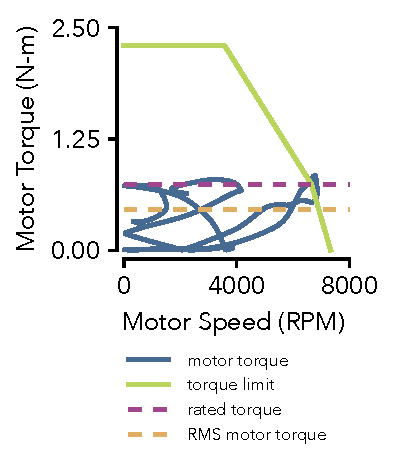
\includegraphics[width=\linewidth]{ankle_motor_torque_running}
    \caption{Ankle motor torque required to reproduce the running trajectory
    recorded by \citet{novacheck1998biomechanics} assuming a parallel spring
    stiffness of $\unitfrac[267]{N \cdot m}{rad}$ and a gear efficiency of
    $75\%$.
    }\label{fig:ankle_motor_torque_running}
\end{marginfigure}

\Cref{fig:ankle_design} shows an internal view of the ankle actuator and
external views of the actuator and foot mechanism. In the ankle design, the
output of the actuator actuates the foot through a four-bar mechanism. The
actuator pulls or pushes on the proximal end of a length-adjustable tendon. The
distal end of the tendon attaches to one end of a fiberglass series elastic leaf
spring that is also connected to the foot. By measuring the angles of the ankle
actuator output and the ankle joint and using the equations of the four-bar
mechanism's kinematics, we can calculate the deflection of the leaf spring and
thus the torque applied to the ankle.
\begin{figure*}[b!]
    \centering 
    \includegraphics[width=\linewidth]{ankle_design}
    \caption{Internal and external design of the ankle 
    joint.}\label{fig:ankle_design}
\end{figure*}

The design of the ankle actuator represents a second iteration of the knee
actuator design and features two main improvements.  First, it has increased
space on the side of the motor for cable routing. Second, the ankle actuator has
a solid rotor shaft. In contrast, the knee actuator's shaft is comprised of two
parts: one that held the motor rotor and transferred power through the gear set,
and another that held the sin/cos encoder's magnetic shaft component. In
practice, these two components proved difficult to align, causing degraded
performance of the sin/cos encoder. The ankle actuator's solid shaft ensures the
encoder magnet stays aligned with the read head.

\begin{marginfigure}[-0.0in]
    \centering 
    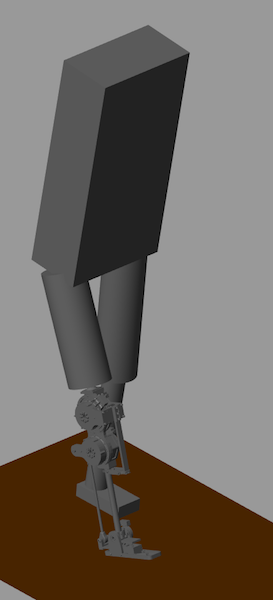
\includegraphics[height=2in]{ankle_impact_sim}
    \caption{Impact simulation we used to determine appropriate series spring
    stiffness.}\label{fig:ankle_impact_sim}
\end{marginfigure}
As we did for the knee series spring, we again determine an acceptable ankle
spring stiffness by performing an impact simulation. For the ankle, we simulate
an \unit[80]{kg} person stepping on the prosthesis when the motor driver
provides the ankle motor with zero applied voltage. \Cref{fig:ankle_impact_sim}
shows the simulation environment. From this simulation we find that a spring
stiffness of about $\unitfrac[1000]{N \cdot m}{rad}$ should sufficiently protect
the ankle gear set from impacts. This estimate is likely softer than necessary
due to the additional series compliance in the amputee's socket and the
composite foot that are not included in the simulation.

\section{Experiments on Powered Knee/Passive Ankle
Prosthesis}\label{sec:complete_exp} 

\emph{Material in this section based partially on
\citet{thatte2016toward}\cite{thatte2016toward}}
\linebreak

Towards a full realization and study on amputee subjects, we present a partial
implementation and evaluation of the control on the current prosthesis prototype
worn by a non-amputee user. \Cref{fig:test_bed_annotation} shows an able-bodied
user wearing our current prosthesis prototype. The current prosthesis prototype
has an active knee SEA unit and an unpowered, spring-loaded, ankle.  We connect
the prosthesis to a knee crutch (iWalk 2.0 Hands Free Crutch) in order to allow
a non-amputee experimenter to test the control. Additionally, the experimenter
wears a lift shoe to compensate for the added thigh length of the knee crutch
and prosthesis.
\begin{figure}
    \centering 
    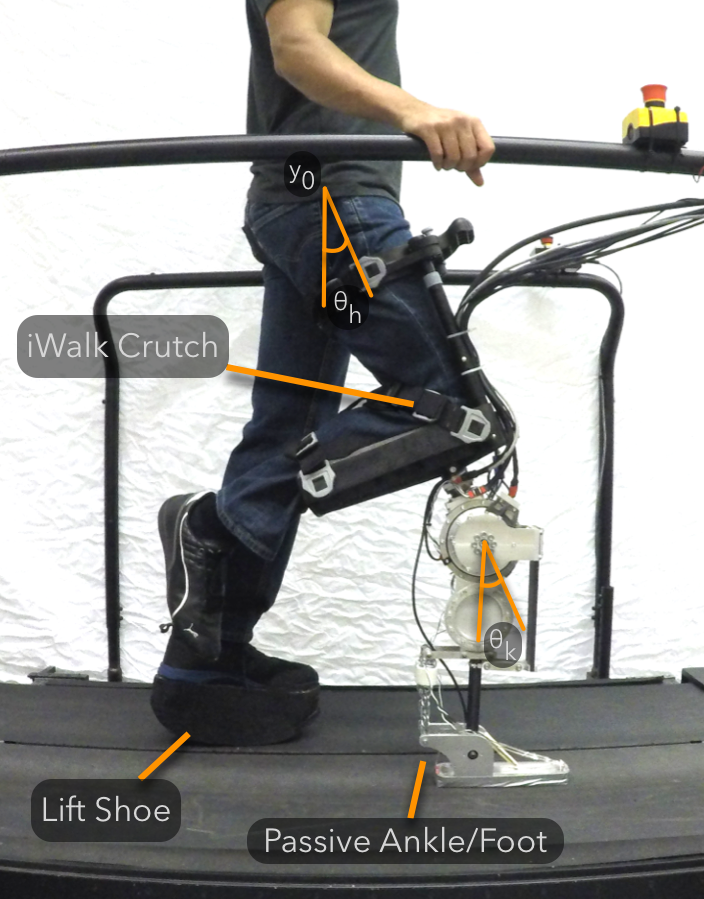
\includegraphics[height=3in]{test_bed_annotation}
    \caption{A non-amputee experimenter tests the prosthesis using an iWalk
    Crutch as a knee adaptor. The experimenter wears a lift shoe on the
    contralateral leg to compensate for the added thigh length of the prosthesis
    and knee adaptor.
    }\label{fig:test_bed_annotation}
\end{figure}

To control the prosthesis knee, we use Simulink Real-Time (Mathworks, USA),
which samples all sensors (joint encoders, IMU on thigh, force sensors in foot),
runs a velocity-based SEA control \citep{schepelmann2012development}, and sends
commands to the motor controller at a rate of 1kHz. Given a desired torque,
$\tau_\tn{d}$, and a measured torque error, $\tau_\tn{e}$, the commanded motor
velocity is given by
\begin{align}
    \omega_\tn{m} = \frac{1}{k} \frac{\tn{d} \tau_\tn{d}}{\tn{d} t} 
        + (1 + k_\tn{d})\omega_\tn{l} + \func{PD}{\tau_\tn{e}},
    \label{eq:velocity_based_sea}
\end{align}
where $\omega_\tn{l}$ is the velocity of the load-side of the series spring (the
shank), $k_\tn{d}>0$ compensates for damping in the knee bearing, and
$\func{PD}{\cdot}$ is a proportional-derivative feedback term. 

The behavior control of the knee is a hybrid model that combines the
Neuromuscular Stance control described in \cref{sec:neuro_stance_reflexes} with
the idealized swing control outlined in \cref{sec:neuro_ideal_swing}. The
missing ankle actuation in the current prosthesis prototype restricts the
neuromuscular stance control to those muscles that span the knee: the vastus,
hamstring, and gastrocnemius. The hamstring and vastus are stimulated according
to \cref{eq:ham_stim_full,eq:vas_stim_full} respectively.  Similarly, the
gastrocnemius is stimulated by positive force feedback. (The torso balance
contribution of the complete hamstring stimulation, \cref{eq:ham_stim_full}, is
neglected.) The realtime software executes the hybrid neuromuscular behavior
control at a rate of 5kHz, ensuring that the integration (ode1) of the simulated
muscle dynamics remains stable. During swing, we only use the knee portion of
the swing control given by \crefrange{eq:flexphase}{eq:extend}. In late swing,
the control transitions between the two phases in proportion to the measured
ground reaction force (\cref{eq:stance_grf_trans,eq:swing_grf_trans}).

% Generation of normal stance behavior
\subsection{Slow Walking Behavior}\label{sec:completed_knee_exp_walk}
We first test if the prosthesis control can reproduce normal stance and swing
behavior of the lower limb in steady-state walking. For this purpose, we capture
joint kinematics and kinetics as well as the virtual muscle activations of the
prosthesis control while an experimenter walks for ten trials with the crutch
and prosthesis system on a treadmill. Because the fit of the crutch to the
experimenter's leg is not very tight, we limit the walking speed to
\unitfrac[0.5]{m}{s} and the experimenter holds onto handrails for safety
(\cref{fig:test_bed_annotation}).
\begin{figure}[t]
    \centering
    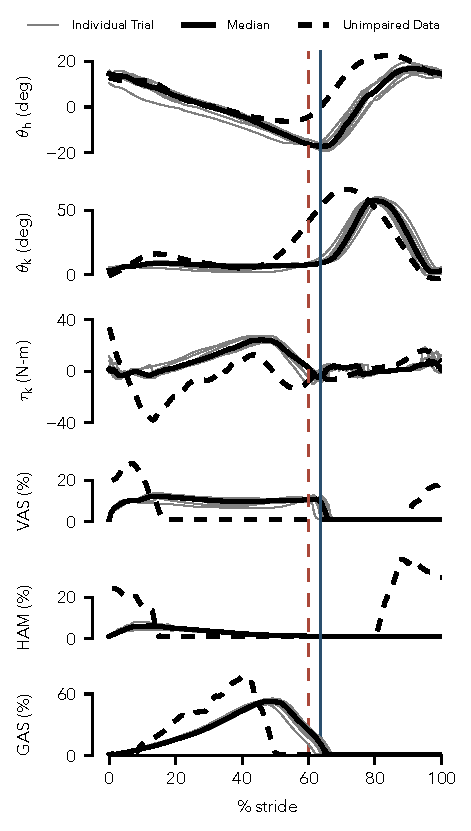
\includegraphics[width = 3in]{pros_gait_data}
    \caption{Prosthesis behavior at walking speed of 0.5 m/s. Shown are the hip
    and knee trajectories, the knee controller torque, and the activations of
    the vastus, hamstring, and gastrocnemius muscles generated by the
    prosthesis control in the testbed. Solid black lines show averaged data  of
    ten trials with the individual trials depicted in gray. Dashed lines show
    corresponding data from human walking at preferred speed (joint angles and
    knee torque: \citet{winter2009biomechanics}, muscle surface
    electromyograms: \citet{perry2010gait}). Solid and dashed vertical lines
    indicate median toe off times for the prosthesis and human data
    respectively.
    }\label{fig:pros_gait_data}
\end{figure}

The control generates steady-state prosthesis behavior that qualitatively
reproduces human leg behavior in walking. \Cref{fig:pros_gait_data} compares the
observed prosthesis leg behavior (solid lines) to corresponding human data at
preferred walking speed (dashed lines, adapted from
\citet{winter2009biomechanics,perry2010gait}). The hip and knee kinematics match
overall, although later transitions from stance to swing are observed in both
joints ($\theta_\tn{h}$ and $\theta_\tn{k}$) and the prosthesis knee flexes less
in stance ($\theta_k$). The knee torque follows trends similar to human data,
but the peak flexion and extension torques in the early stance phase are
diminished ($\tau_\tn{k}$). These lower peaks are caused by reduced activations
of the virtual vastus and hamstring muscles (VAS and HAM) in this phase, a clear
difference to these muscles' activation in humans, in which bursts of activity
at heel strike are followed by relative silence. Finally, the activity of the
virtual gastrocnemius muscle (GAS) bears strong similarity the activity of this
muscle in human walking.

To some extent, limitations of our current experimental testbed may
account for observed discrepancies. The imposed slow walking speed of 0.5 m/s
required less energy absorption in early stance than at normal walking speed.
Moreover, the experimenter held onto the handrails to assist with lateral
balance, which may have channeled some impact energy through the arms. In
addition, the hybrid nature of the proposed control prevents the virtual
muscles from activating in swing, which is the case in humans
(\cref{fig:pros_gait_data}, VAS and HAM activities from 80\% to 100\% of gait
cycle), and would alter the response of the virtual muscles at heel strike.
Finally, the lack of an active ankle and its control in the current prosthesis
prototype further limits how closely the leg behaviors can match.

% Response to Swing Leg Tripping
\subsection{Response to Swing Leg Tripping}\label{sec:completed_exp_swing_trip}
 

In a second set of experiments, we evaluate the response of the prosthesis
controller to trip disturbances. We apply disturbances during treadmill walking
by commanding flexion knee torques to the prosthesis in addition to its
swing-leg control torque. The added torque simulates an obstacle encounter
modeled in the same way as the stopping torque of the swing leg control,
\cref{eq:stop}, with $\alpha_{thr}$ replaced by a disturbance leg angle. The
foot can pass the simulated obstacle if the leg length contracts beyond a
threshold of \unit[94]{cm}. For an early-, mid-, or late-swing encounter, the
disturbance angle is set to 110, 95, or \unit[80]{degrees}, respectively. In
addition, anticipation of the trip by the experimenter is prevented by applying
the disturbance only with a probability of 25\%.

\begin{marginfigure}[1in]
    \centering
    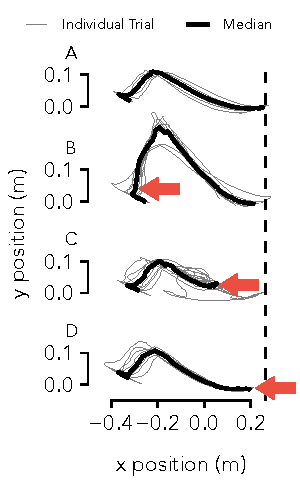
\includegraphics[width = \linewidth]{impulse_hardware_annotated.pdf}
    \caption{Response to simulated tripping disturbance. (A) Undisturbed ankle
    trajectory calculated from hip and knee angles assuming constant hip height.
    (B-D) Ankle trajectories with disturbance applied in early, mid and late
    swing (arrows). The vertical dashed line shows the target landing position
    of the foot, which corresponds to a \unit[75]{degree} landing angle.}
    \label{fig:impulse_hardware}
\end{marginfigure}

The experiments reveal that in response to disturbances during early and late
swing, the prosthesis control places the swing leg with high repeatability and
produces leg elevating and lowering strategies observed in humans.
\cref{fig:impulse_hardware} shows the Cartesian ankle trajectory in swing over
10 trials for the undisturbed (A) and disturbed conditions (B-D). In the
undisturbed condition, the leg placement is repeatable with an interquartile
range (IQR) of landing positions of \unit[3.1]{cm} and a bias of \unit[2.7]{cm}
(median) from the target (dashed line).  (Further tuning of the control
parameters should improve the landing position accuracy.)

In the early disturbance condition (\cref{fig:impulse_hardware}B), the
prosthesis generates large knee flexion roughly doubling the peak ground
clearance. Nonetheless, the median landing position remains within
\unit[5.3]{cm} of the target (IQR: \unit[10.2]{cm}), demonstrating the knee
control's ability to compensate for early swing disturbances. This response is
similar to the leg elevating strategy observed in humans when disturbed shortly
after toe-off \citep{eng1994strategies, schillings2000muscular}. The biological
strategy, however, shows active knee flexor muscle contributions, while the
prosthesis knee flexion is entirely passive, as the leg angular velocity does
not become negative during the disturbance (Eq.~\ref{eq:flexphase},
\cref{sec:neuro_ideal_swing}).

In the late disturbance condition \cref{fig:impulse_hardware}D),
the prosthesis leg behavior resembles the lowering strategy of
humans~\citep{schillings2000muscular}, in which knee extensor muscles quickly
extend the leg. This behavior is triggered on the prosthesis in the third phase
of the swing control before the leg angle starts to retract
(\cref{eq:extend}). The prosthesis achieves ground contact slightly earlier
with a median landing point of \unit[8.8]{cm} before the target (IQR:
\unit[3]{cm}).

Finally, \cref{fig:impulse_hardware}C shows the response of the
prosthesis to a mid-swing disturbance. When humans are confronted with
disturbances in mid swing, they may use either elevating or lowering strategies
\citep{eng1994strategies, schillings2000muscular}. However, the prosthesis
response resembles neither strategy. During mid swing, the prosthesis control
uses a holding policy, damping both knee flexion and extension
(\cref{eq:holdphase}). Consequently, in most cases the knee angle neither
flexes adequately to clear the obstacle nor extends quickly enough to make
timely ground contact. In these trials, falling was only prevented via support
from the treadmill handrails.

\section{Comparison of Robustness Achieved by Reflex and Impedance Controls in
    Simulation}\label{sec:completed_comparison}

\emph{Material in this section based partially on 
\citet{thatte2016toward}\cite{thatte2016toward} 
and \citet{thatte2014towards}\cite[0.25in]{thatte2014towards}}
\linebreak

To evaluate the potential of neuromuscular prosthesis control to improve amputee
gait robustness, we construct a simulation of an amputee walking on a powered
prosthesis and perform optimizations to identify parameters that lead to robust
locomotion over rough terrain. We then compare the performance of the proposed
control to that of impedance control and find that the proposed control improves
robustness to elevation changes and unexpected deviations from nominal walking,
suggesting that it may help amputees prevent trips and falls
(\cref{fig:distsWalked}).

\subsection{Simulation Environment}\label{sec:complete_simulation_environ}
We study the performance of the proposed transfemoral prosthesis controller in a
simulation model of a unilateral amputee equipped with the proposed powered
prosthesis. To more accurately model an amputee's anatomy, we sever the femur of
the unimpaired human model \unit[11]{cm} above the knee and attach the hamstring
muscle to the distal end of the shortened bone as recommended in
\citet{brown2012amputation}. This change converts the biarticular hamstring into
a monoarticular muscle that only extends the hip. Next, we attach a model of the
full prosthesis to the severed femur. The prosthesis modeled in this study is an
earlier version of the prosthesis design presented in
\cref{sec:completed_design}, which uses the knee actuator design for both the
knee and ankle joints. Our simulation of the prosthesis models the series
elasticity, electrical dynamics, gear ratios, and resultant reflected inertias
of the actuators, and assumes a low-level current-based SEA control achieves
desired torques \citep{pratt1995series}.

To generate the reference torques for the SEAs, we use a hybrid neuromuscular
control that blends the muscle based stance-control
(\cref{sec:neuro_stance_reflexes}) with the idealized swing leg placement
control \cref{sec:neuro_swing_reflexes}. We make make two modifications to the
prosthesis-side swing leg control.  First, on the prosthesis-side hip we remove
the feed-forward term that neutralizes the disturbance created by the knee's
stop and extend phase (\cref{eq:hipfeedforward}), requiring that feedback
control deal with this torque.  Second, we do not use the adaptive leg placement
policy of the swing control (\cref{eq:simbicon}) as the prosthesis does not have
access to information about the amputee's center of mass and stance leg ankle
position.  Instead the prosthesis swing leg control employs a constant target
leg angle, $\alpha_\tn{tgt} = const$.

To compare the performance of the proposed control, we also simulate the
commonly-used impedance control method, described in detail in
\cref{sec:back_dynamic_pros_control}, at the behavior level.  Specifically, we
implement the impedance control presented in \citet{sup2008design} as it tended
to perform better than other versions in our simulations. This control
partitions the gait cycle into four phases. In each phase $i$, the torque of an
actuated joint is governed by an impedance function
\begin{align} 
    \tau_i = -k_{1,i} (\theta - \theta_{1,i}) - k_{2,i} 
        (\theta - \theta_{2,i})^3 - b_i \dot{\theta} , 
\end{align} 
where $\theta$ is the joint angle, $\theta_{1,i}$ and $\theta_{2,i}$ are angle
offsets, and $k_{1,i}$, $k_{2,i}$ and $b_i$ are the impedance parameters.  

% Parameter Optimization
\subsection{Controller Optimization for Natural and Robust Walking}
    \label{sec:completed_comparison_opt}

For both the hybrid neuromuscular controller and the impedance controller, we
use optimization to search for gaits that appear natural and are robust to
disturbances. For the hybrid neuromuscular model, we optimize 53 parameters that
include reflex feedback gains and swing leg control parameters for both the
amputee and prosthesis as well as the SEA control gains. To reduce the number of
parameters to optimize, we use fixed values for many parameters, such as the
muscle properties and prestimulations. For the impedance controller, we optimize
59 parameters that include the reflex feedback gains and the swing leg control
parameters for the amputee model, and the impedance parameters and SEA
controller gains for the prosthesis. Again to reduce the number of parameters to
optimize, the impedance parameters that are set to zero according to
\citet{sup2008design} are fixed to zero during the optimization. 

We rely on the covariance matrix adaptation evolution strategy (CMA-ES)
\citep{hansen2006cma} and perform optimization in two steps. In the first step,
we search for control parameters that generate a gait with natural kinematics
and kinetics. To this end, we take advantage of the observation that human gait
seems to result from minimizing metabolic energy consumption
\citep{mcneill2002energetics}, and use the cost of transport 
\begin{align}
    \mathit{Cost} = \frac{W}{mgx} + \frac{1}{mgx} \int \left( 
        c_1\tau_\tn{cmd}^2  + c_2 \tau_\tn{limit}^2 \right) \tn{d}t
    \label{eq:costfuncenergy}
\end{align}
as optimization criterion. In the cost, $W$ accounts for the energy consumption
of both the modeled amputee's muscles and the prosthesis' virtual muscles
according to \citet{umberger2003model}, $\tau_\tn{cmd}$ is the sum of the
torques commanded by the neuromuscular swing control or the impedance control,
$\tau_\tn{limit}$ is the sum of torques produced by the model's mechanical
hardstops, which prevent knee and ankle hyperextension, $m$ is the mass of the
amputee, $g$ is the gravitational acceleration, and $x$ is the distance
travelled in 20 seconds. The hand tuned constants, $c_1 = 0.1$ and $c_2 = 0.01$,
ensure that the terms of the cost function have similar order-of-magnitude. 

We run the above optimization for 300 iterations, and use the best resulting set
of control parameters to seed an optimization for robustness to unexpected
changes in ground height. For this second step, the cost function becomes
\begin{align}
    \mathit{Cost} = -x + c_3 \int \tau_\tn{limit}^2 dt ,
\end{align}
rewarding the distance travelled and penalizing joint hyperextension ($c_3 =
0.0005$). Instead of level ground, the simulations evaluating the cost are
performed on terrain that is flat for the first 10 meters (to allow the model to
reach steady walking) and then features steps, spaced one meter apart and drawn
from a uniform random distribution. The width of the distribution grows at a
rate of \unit[2.5]{cm} per meter distance travelled, resulting in steps that
grow progressively rougher the farther the model walks. To avoid overfitting,
the evaluation is performed on five different terrains, resulting in an average
cost. Like in the first step, the optimization is stopped after 300 iterations,
resulting in the final, best set of control parameters.

\subsection{Results}\label{sec:completed_comparison_results}
\begin{figure}[t]
    \centering
    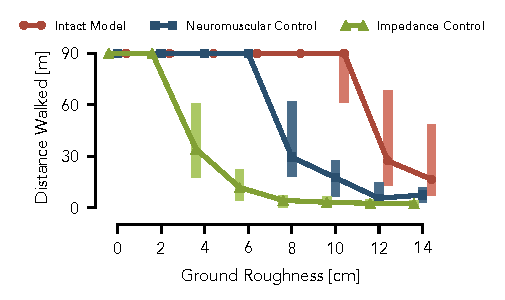
\includegraphics[width = \columnwidth]{distsWalked}
    \caption{Control performance of simulated prosthesis on rough terrain. The
    distances walked over terrains with different ground roughness are compared
    between the amputee model using a powered knee-ankle prosthesis with
    impedance control (green) and hybrid neuromuscular control (blue) as well
    as with the unimpaired human model (red). Shown are the median and range
    ($25^\textrm{th}$ and $75^\textrm{th}$ percentiles) of the covered
    distances for 50 terrains sampled at each roughness level.
    }\label{fig:distsWalked}
\end{figure}

We evaluate the performance of the proposed control and of impedance control by
subjecting the amputee model to terrains that are flat for \unit[10]{meters} and
then feature steps drawn from uniform distributions for another
\unit[90]{meters}.  The widths of the distributions are constant but vary among
the terrains to test the control performance on steps of increasing steepness
(\unit[0]{cm} to $\pm \unit[14]{cm}$, \unit[2]{cm} increments, total of 8
terrains). 

\Cref{fig:distsWalked} shows the distances the amputee model walks over 50
trials at each roughness level (proposed neuromuscular control in blue,
impedance control in green). Most of the trials with the impedance-controlled
prosthesis cover the full distance up to a roughness of \unit[2]{cm}. At a
roughness of \unit[4]{cm}, however, the median distance drops to \unit[34]{m},
which further declines as the roughness increases. In contrast, the  prosthesis
using the neuromuscular control, allows the amputee model to walk the full
distance up to a roughness of \unit[6]{cm}. Moreover, neuromuscular control has
a similar distribution of distances walked at a roughness of \unit[8]{cm} as
impedance control has at a roughness of \unit[4]{cm}.

Although the prosthesis using neuromuscular control significantly improves the
robustness of the amputee model on rough terrain, the performance trails by a
large margin that of an unimpaired model (\cref{fig:distsWalked}, red line), for
which most of the trials covered the full distance up to a roughness of
\unit[10]{cm}.  Limiting the swing leg placement targets in the neuromuscular
prosthesis control to constant angles may account for some of this performance
gap. In future work, we may overcome this limitation by estimating the amputee's
center of mass velocity and stance ankle position so that the prosthesis control
can take advantage of the full leg placement policy (\cref{eq:simbicon}). Other
sources for the performance gap could stem from differences in the inertial
properties between the prosthesis and the healthy leg, delay and inaccuracy in
the series elastic actuator torque tracking, and the increased number of
parameters in the asymmetric amputee model, which can reduce the quality of the
optimized solutions.

A possible explanation for why the neuromuscular control produces more robust
behavior than impedance control is the former's attempt to mimic the underlying
dynamics and goals of human motor control rather than to track impedance
behavior about a predefined motion for each individual joint. To illustrate this
difference, we subject the amputee model with both control strategies to a
simulated trip in the form of a $\unit[15]{N \cdot s}$ impulse applied at 5\% of
the undisturbed swing duration. 

\begin{figure*}[t]
    \centering
    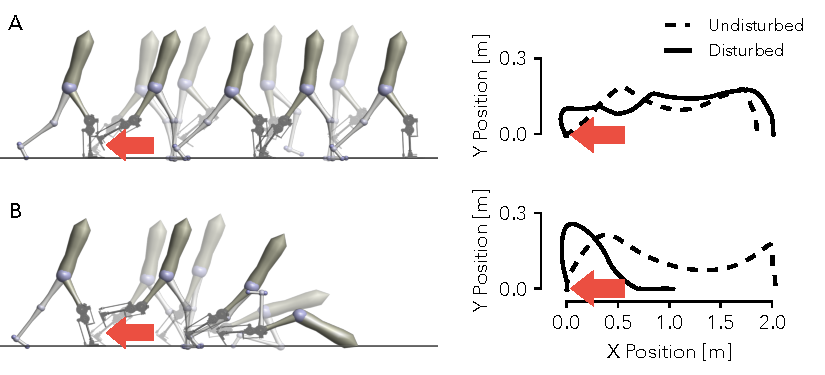
\includegraphics{impulseResponseAnnotated}
    \caption{Tripping response of the amputee model with neuromuscular (A) and
    impedance control (B) of the prosthesis. Shown are the prosthetic toe
    trajectories during undisturbed gait (dashed line) and when disturbed by a
    $\unit[15]{N \cdot s}$ impulse (solid line). The neuromuscular controller
    effectively responds to the disturbance and maintains a qualitatively
    similar toe trajectory. The impedance controller leads to foot scuffing and
    an eventual fall.
    }\label{fig:ImpulseResponses}
\end{figure*}

\Cref{fig:ImpulseResponses}A shows the toe trajectory of the prosthesis using
neuromuscular control both in the undisturbed and disturbed cases. While the
impulse causes a large deviation from the nominal trajectory in early swing, the
controller quickly recovers. From mid-swing onward, the foot follows a
qualitatively similar path, maintains adequate ground clearance, and
successfully reaches a similar foot placement as in the undisturbed case. In
contrast, the prosthesis with impedance control does not respond adequately when
subjected to the disturbance (\cref{fig:ImpulseResponses}B). This is illustrated
by the prosthesis behavior in mid swing, during which it does not react
appropriately to maintain ground clearance of the toe. Rather, the joint-based
impedance functions drive the knee into extension prematurely, and the
prosthetic foot scuffs the ground resulting in a trip and subsequent fall.

\subsection{Discussion}\label{sec:completed_comparison_discuss}

Our simulation results suggest that the hybrid neuromuscular control policy can
improve amputee gait stability over existing impedance control methods. An
amputee model walking with a powered prosthesis showed substantial improvements
in balance recovery on rough ground and after swing leg trips when using the
hybrid neuromuscular control policy as opposed to impedance control.  One
possible reason for the improvement is that the proposed controller considers
global leg information such as the target leg angle
(\crefrange{eq:flexphase}{eq:stop}), and it is well known that without placing
the feet into proper target points on the ground, legged systems fail to balance
\citep{townsend1985biped,raibert1986legged,kajita20013d,
seyfarth2002movement,pratt2006capture,wu20133}. A second reason could be that
the design of the swing leg control policy explicitly accounts for large
disturbances to the lower limb dynamics in order to achieve desired leg
placements \citep{desai2012robust}. Neither is the case for current impedance
control policies; however, future research may show that impedance or other
control policies can equally make use of this global information and design
criterion.

Whether the simulation results transfer to amputee gait remains to be
determined. In an initial test with a non-amputee experimenter wearing the
prosthesis via a knee adaptor, we found the hybrid neuromuscular control
reproduces normal walking patterns qualitatively and effectively responds to
disturbances in early and late swing. To understand if these initial results
generalize to amputee locomotion requires further research. First, we only
simulated disturbances in the hardware tests by commanding disturbance torques
to the prosthesis knee. This approach allowed us to apply reproducible
disturbances, but it does not capture real tripping or obstacle encounters,
which will, for instance, exert torques about the hip joint as well.  Second,
the use of the knee adaptor creates abnormal kinematics and inertias and
provides only a loose fit between user and prosthesis. In consequence, we only
tested slow walking at 0.5 m/s holding onto hand rails.

Finally, the simulation and hardware tests captured only a small
portion of the balance disturbances that humans typically encounter
\citep{robinovitch2013video}. Other disturbances may evoke amputee responses
that the simulation model does not capture; especially since it is driven
solely by a reflexive walking controller that ignores conscious interventions.
Already, the hardware experiments revealed that the control's response to
mid-swing disturbances does not match observed human responses and risks
allowing the user to fall. This result suggests the model and corresponding
hardware implementation require additional reflexes or structural changes in
the control to better capture human locomotion and balance recovery. Foot
placement into target points, while beneficial in particular for responding to
early swing disturbances and for rough ground walking, may not be a goal that
the human system prioritizes in response to other disturbances. Identifying
human objectives in these situations could lead to improved leg prosthesis
behaviors independent of the proposed approach, impedance-like approaches, or
other control design approaches.


\section{Optimization of Systems Using
Preferences}\label{sec:completed_pref_opt}

\emph{Material in this section based on
\citet{thatte2017sample} (in review) \cite{thatte2017sample}} 
\linebreak
 
As discussed in \cref{sec:back_optimization} previous work has explored learning
from qualitative feedback such as preferences in order to circumvent defining
objective functions and using Bayesian optimization in order to reduce the
number of experiments requried to optimize a system. In this section, we present
a new optimization algorithm, Predictive Entropy Search with Preferences
(PES-P), that combines these two ideas. The algorithm uses preference queries
between pairs of control parameters to avoid the a priori definition of features
and to consider unquantifiable qualities of the desired behavior. The algorithm
further incorporates black-box Bayesian optimization to ensure its preference
queries gather information efficiently without relying on a system model.

In developing the algorithm, we make three main contributions. First, we adapt
an acquisition function previously proposed for interval scale feedback to the
preference feedback case. This acquisition function seeks a pair of parameters
for which a preference will maximally reduce the entropy of the distribution of
objective function optima. Second, we compare in simulation the performance of
the proposed optimization method against the expected improvement method (EI)
and uniform random sampling via Latin hypercubes (LH) for two classes of
examples: optimizing randomly generated objective functions and tuning the
control parameters of simulated dynamical systems.  Finally, we compare the
performance of the three methods for the task of optimizing the control
parameters of a robotic prosthesis given real user feedback.

\subsection{Preliminaries} 
\subsubsection{Learning from Preferences}

To learn latent objective functions from preferences, we rely on the method
developed by \citeauthor{chu2005preference}~\citep{chu2005preference}, briefly
reviewed here.  The method considers a training dataset $D_n$ of $n$ preferences
between pairs of points, $\{x_1^\tn{a} \succ x_1^\tn{b}, \ldots, x_k^\tn{a}
\succ x_k^\tn{b}, \ldots, x_n^\tn{a} \succ x_n^\tn{b}\}$. These points can, for
instance, represent control policy parameters. From the dataset, the method
finds a posterior distribution of latent objective functions $\vecf{f}$,
\begin{align}
    \prob{\vecf{f}|D_n} = \frac{\prob{D_n|\vecf{f}}
        \prob{\vecf{f}}}{\prob{D_n}}.
    \label{eq:bayes_rule}
\end{align}
where $\vecf{f} = [f(x_1^\tn{a}), f(x_1^\tn{b}), \ldots, f(x_n^\tn{a}),
f(x_n^\tn{b})]^T$. First, the method assumes that the prior distribution of
objective functions is a zero-mean \emph{Gaussian process} (GP),
$\prob{\vecf{f}} = \mathcal{N}(0, \Sigma)$. An appropriate kernel, $\Sigma_{i,j}
= \func{k}(x_i,x_j)$, describes the elements of the covariance matrix $\Sigma$.
(See~\citep{williams2006gaussian} for a full description of GPs.) Second,
$\prob{D_n|\vecf{f}}$ is the overall likelihood of preferences in the
dataset given specific reward function values and is modeled as the product of
the likelihood of each independent preference in the dataset,
\begin{align}
    \prob{D_n|\vecf{f}} &= \prod_{k=1}^n \prob{x_k^\tn{a} \succ x_k^\tn{b} 
            | f(x_k^\tn{a}), f(x_k^\tn{b})} 
        = \prod_{k=1}^n \Phi(q_k),
    \label{eq:likelihood}
\end{align}
where $\prob{x_k^\tn{a} \succ x_k^\tn{b} | f(x_k^\tn{a}), f(x_k^\tn{b})}$ is the
probability of a preference if Gaussian noise with variance $\sigma^2$ corrupts
the function values, $\Phi(\cdot)$ is the cumulative distribution function of a
normal distribution, and $q_k = \frac{f(x_k^\tn{a}) - f(x_k^\tn{b})}{\sqrt{2}
\sigma}$.  In essence, the likelihood model increases the certainty of a
preference between $x_k^\tn{a}$ and $x_k^\tn{b}$ as the difference between
$f(x_k^\tn{a})$ and $f(x_k^\tn{b})$ widens. 

To obtain the posterior distribution $\prob{\vecf{f}|D_n}$ the method
approximates \cref{eq:bayes_rule} with a Gaussian distribution. As a result, the
predictive distribution (subscript p) of the objective function at test points,
$\vecf{f}[\tn{t}]$, is also Gaussian, $\prob{\vecf{f}[\tn{t}] | D_n} =
\mathcal{N} \left( \mu_\tn{p}, \Sigma_\tn{p} \right)$. Finally, the predictive
distribution of a preference between two points $x^\tn{a}$ and $x^\tn{b}$ is 
\begin{align} 
    \prob{x^\tn{a} \succ x^\tn{b} |D_n} 
    &=\hspace{-2pt}\int \prob{x^\tn{a} \succ x^\tn{b}|\vecf{f}[\tn{t}],D_n}
    \prob{\vecf{f}[\tn{t}]| D_n} \tn{d} \vecf{f}[\tn{t}] 
        \label{eq:prob_of_pref}\\
    &= \Phi \left(\frac{\mu^\tn{a} - \mu^\tn{b}}{\sigma_\tn{p}} \right),
        \label{eq:p_pref} \\ 
    \sigma_\tn{p}^2 &= 2\sigma^2 + \Sigma_\tn{p}^\tn{aa} + \Sigma_\tn{p}^\tn{bb}
        - \Sigma_\tn{p}^\tn{ab} - \Sigma_\tn{p}^\tn{ba}.
\end{align}

\Cref{fig:pes_plot}a provides an example of how the method estimates a
ground-truth objective function shown in purple. The blue line and shaded area show
the mean and standard deviation of the posterior distribution of objective
functions, $\prob{\vecf{f}_\tn{t}|D_n}$, after two preference queries between
pairs of parameters (orange, higher is preferred over lower value). The queries
have the effect of lifting the estimated objective function close to preferred
points and pushing it down close to unpreferred points, approximating the true
objective function over time.

\subsubsection{Active Learning for Optimization}
Learning from preferences describes how to find a distribution of objective
functions given a dataset of comparisons. The question now becomes how to
efficiently solicit preferences from the user. As our main goal is to find the
optimal parameters $x^*$, we should forgo modeling the objective function
accurately in all parameter regions and instead focus on regions where the
objective might be high. Bayesian optimization addresses this problem with an
acquisition function that helps to efficiently sample training data.
\begin{marginfigure}
    \centering
    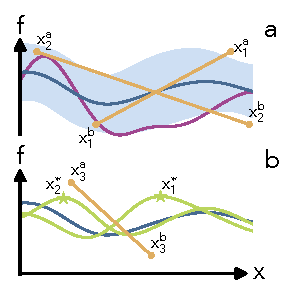
\includegraphics[width=\linewidth]{pes_plot}
    \caption{Learning from preferences. (a) Mean and standard deviation of
    $\prob{\vecf{f}[\tn{t}]|D_n}$ (blue) after two preferences queries (orange)
    from the true objective function (purple). (b) Mean of
    $\prob{\vecf{f}[\tn{t}]|D_n}$ (blue) and means of
    $\prob{\vecf{f}[\tn{t}]|D_n, x_m^*}$ (green) for two samples of $x_m^*$.
    PES-P queries a new comparison (orange) for which the preference is
    currently uncertain, but on average is certain after conditioning on all
    $x_m^*$.}\label{fig:pes_plot}
\end{marginfigure}

One such acquisition function is the expected improvement, which has been used
both in the context of preference feedback~\citep{eric2008active} and interval
scale feedback~\citep{jones1998efficient},
\begin{equation}
    \func{EI}{x} = (\mu^* - \mu(x))\Phi(d) + s(x)\phi(d),
    \label{eq:expected_improvement}
\end{equation}
where $d = (\mu^* - \mu(x))/s(x)$, $\mu^*$ is the mean of the current estimate
of the optimum, and $\mu(x)$ and $s(x)$ are the mean and standard deviation of
the objective of a new point $x$, respectively. As an alternative, for interval
scale feedback,~\citep{hennig2012entropy} and~\citep{hernandez2014predictive}
proposed acquisition functions that seek to reduce the uncertainty in the
distribution of objective function optima, measured in terms of the differential
entropy. For example, the Predictive Entropy Search acquisition
function~\citep{hernandez2014predictive} seeks a point $x$ that is expected to
reduce the entropy of the distribution of optima $x^*$ after observing its value
$y$,
\begin{align}
    \alpha_n \left(x \right) = \funcsb{H}{\prob{x^*|D_n}} 
        - \funcsb{E}[\prob{y|x, D_n}]{\funcsb{H}{\prob{x^*|y, x, D_n}}},
    \label{eq:pes_interval_scale}
\end{align}
where $\funcsb{H}{\prob{x}} = - \int \prob{x} \log \prob{x} \tn{d} x$
is the differential entropy. The authors of these methods have shown they can
outperform EI\@. 

% -------
% Methods
% -------
\subsection{Methods}
Our goal is to simultaneously address both the difficulty of defining objective
functions when an expert cannot demonstrate the desired robot behavior and the
expense of running experiments on hardware. To this end, we adapt the Predictive
Entropy Search acquisition function (\cref{eq:pes_interval_scale}) to the
preference learning case.

\subsubsection{Acquisition Function}
To obtain the optimal parameters $x^*$ with the smallest number of preference
queries, we solicit preferences that maximize the expected information gain
about the distribution of objective function optima $\mathrm{P}(x^*|D_n)$.
Adapting \cref{eq:pes_interval_scale} to preference feedback yields
\begin{fullwidth}
\begin{align}
    &\alpha_n \left(x^\tn{a}, x^\tn{b}\right) 
        = \funcsb{H}{\prob{x^*|D_n}} - \funcsb{E}[\prob{y|x^\tn{a},x^\tn{b},D_n}]
            {\funcsb{H}{\prob{x^*|y, x^\tn{a}, x^\tn{b}, D_n}}},
    \label{eq:acquisition_orig}
\end{align}
\end{fullwidth}
where $y$ is a binary random variable that represents the preference between
$x^\tn{a}$ and $x^\tn{b}$. The first term in this function is the current
entropy of objective function optima and the second term is the entropy of
optima after observing the preference $y$. As we have not yet observed the
preference, we take the second term in expectation over the two possible
preference outcomes.

As discussed in~\citep{hernandez2014predictive}, this acquisition function is
intractable to compute. However, following the approach used for the original
PES algorithm, we can rewrite~\cref{eq:acquisition_orig} in terms of the
entropies of the predictive distribution of the preference between $x^\tn{a}$
and $x^\tn{b}$,
\begin{fullwidth}
\begin{align}
    \alpha_n \left(x^\tn{a}, x^\tn{b} \right) &= 
        \funcsb{H}{\prob{y|x^\tn{a}, x^\tn{b}, D_n}}
            - \funcsb{E}[\prob{x^*|D_n}]{\funcsb{H}
            {\prob{y| x^*, x^\tn{a}, x^\tn{b}, D_n}}} \\
        &\approx \funcsb{H}{\prob{y|x^\tn{a}, x^\tn{b}, D_n}}
            - \frac{1}{M} \sum_{x_m^* \sim {\prob{x_m^*|D_n}}}^M 
            \hspace{-0.03in}\funcsb{H}{\prob{y| x_m^*, x^\tn{a},x^\tn{b},D_n}}.
        \label{eq:aq_approx}
\end{align}
\end{fullwidth}
This reformulation significantly improves computability. First, the new
acquisition function uses the entropies of probabilities of preferences, given
by~\cref{eq:p_pref}. Second, we now take the expectation over $\prob{x^*|D_n}$,
which we can perform by sampling $M$ functions from
$\prob{\vecf{f}[\tn{t}]|D_n}$ and optimizing each one to get $M$ samples of
$x^*$ (see Appendix for details). Finally, the second term no longer requires
conditioning the GP on every pair of $x^\tn{a}$ and $x^\tn{b}$ considered during
optimization of the acquisition function.  Instead, we only have to condition
the Gaussian process $M$ times on $(x_m^*, D_n)$.

For the experiments in~\cref{s:results} we choose $M = 12$, which allows us to
construct and optimize $\alpha_n(x^\tn{a}, x^\tn{b})$ in about five seconds,
which is fast enough for our prosthesis application. Although 12 samples of
$x^*$ is not enough to compute an accurate expectation over $\prob{x^*|D_n}$,
interpreting the algorithm as an example of active learning by disagreement may
explain why it still works well.  As shown in~\cref{fig:pes_plot}b, optimizing
the acquisition function chooses a pair $x^\tn{a}$ and $x^\tn{b}$ for which the
preference is currently uncertain, but certain on average after conditioning on
all $x_m^*$. The sampled $x_m^*$ do not necessarily agree on which point is
preferred; hence, after observing the preference, the algorithm can rule out
$x_m^*$ that made the model certain but wrong about the preference. This
intuition is similar to that provided by \citep{houlsby2012collaborative} for
Bayesian active learning by disagreement for GP classifiers.

\subsubsection[Conditioning the Gaussian Process on optima]{Conditioning the
Gaussian Process on $x^*$} The second term on the right side
of~\cref{eq:aq_approx} requires us to compute the distribution of the
preference given the location of the optimum,
\begin{fullwidth}
\begin{align}
&\prob{y| x_m^*, x^\tn{a}, x^\tn{b}, D_n} =
    \int \prob{x^\tn{a} \succ x^\tn{b} | \vecf{f}[\tn{t}], x_m^*, D_n} 
    \prob{\vecf{f}[\tn{t}] | x_m^*, D_n} \tn{d} \vecf{f}[\tn{t}].
    \label{eq:predic_pref_w_constraint}
\end{align}
\end{fullwidth}
It is not directly feasible to condition the predictive distribution on $x^*$,
so instead we turn to approximating this condition with three constraints (see
\hyperlink{sec:appendix}{appendix} for details):

C1: First we impose that $x^*$ is a local maximum by ensuring that the gradient
of $f(x^*)$ is zero and its Hessian is negative definite. We further simplify
the Hessian constraint to only require that the Hessian's off-diagonal elements
are zero and its diagonal elements are less than zero. We implement the gradient
and off-diagonal constraints by conditioning the prior, $\prob{\vecf{f}}$, on
derivative observations as outlined in~\citep{solak2003derivative}. To constrain
the diagonal elements of the Hessian, we amend the likelihood term in
\cref{eq:bayes_rule} by adding terms that penalize Hessians with positive
diagonal elements.

C2: Second, we try to ensure that $x^*$ is also a global maximum by enforcing
that $f(x^*)$ is greater than the function values of all training points sampled
so far. We impose this constraint by adding more preference relations into the
likelihood term in \cref{eq:bayes_rule} between $x^*$ and all training points.

C3: Finally, to further ensure that $f(x^*)$ is a global maximum, we require
that it is also larger than the function values of the two new test points,
$f(x^\tn{a})$ and $f(x^\tn{b})$. Whereas C2 ensures $f(x^*)$ exceeds function
values in areas explored so far, C3 ensures that $f(x^*)$ also exceeds function
values in unexplored regions. We approximate this constraint analytically by
conditioning on the single constraint $f(x^*) > (f(x^\tn{a}) + f(x^\tn{b}))/2$
using the
method detailed in~\citep{xu2010estimation}.
\begin{algorithm}[t]
    \caption{Predictive Entropy Search with Preferences}
    \begin{algorithmic}[1]
        \Procedure{PES-P}{}
            \State{$D_n = \varnothing$}
            \For{$n \gets 0$ \textbf{to} $N-1$}\Comment{$N$ iterations}
            	\State{$F \gets \{\vecf{f}[m] \sim \prob{\vecf{f}[\tn{t}]| D_n} 
                    | m \in [1, M]\}$}
               	\State{$X^* \gets \{\arg \max_x \left(\vecf{f}[m] \right) 
                    | \vecf{f}[m] \in F \}$}
                \State{$(x_{n+1}^\tn{a}, x_{n+1}^\tn{b}) \gets \arg
                    \max_{(x^\tn{a}, x^\tn{b})} 
                    \funcil{\alpha}[n]{x^\tn{a},x^\tn{b};X^*}$}
                \State{$y_{n+1} \gets 
                    \textsc{QueryUserPref}(x_{n+1}^\tn{a}, x_{n+1}^\tn{b})$}
                \State{$D_{n+1}\hspace{-0.25em}\gets\hspace{-0.25em}
                    D_n \cup (x_{n+1}^\tn{a}, x_{n+1}^\tn{b}, y_{n+1})$}
            \EndFor{}
            \State{$\textbf{return} \ x^* \gets \arg \max_x
                \func{mode}{\prob{\vecf{f}[\tn{t}](x)| D_N}}$}
        \EndProcedure{}
        \Statex{}
        \Function{$\alpha_n$}{$x^\tn{a}, x^\tn{b}; X^*$}
            \Comment{acquisition function}
            \State{$h \gets \left\{\funcsb{H}{\prob{y|x^\tn{a}, x^\tn{b}, D_n, 
                \tn{C1}, \tn{C2}, \tn{C3}}} | x_m^* \in X^* \right\}$}
            \State{$\textbf{return} \ \funcsb{H}{\prob{y|x^\tn{a},x^\tn{b},D_n}} 
                - \func{mean}{h}$}
        \EndFunction{}
    \end{algorithmic}\label{alg:pesp}
\end{algorithm}

\subsubsection{Algorithm Summary}
With constraints C1 to C3, at each iteration we can efficiently compute the
acquisition function, \cref{eq:aq_approx}. We summarize the resulting Predictive
Entropy Search with Preferences (PES-P) algorithm as follows (\cref{alg:pesp}):
At each iteration $n$, first, the algorithm samples $M$ objective functions from
the current distribution, $\prob{\vecf{f}[\tn{t}]|D_n}$, and optimizes each one
to generate $M$ samples of $x^*$ (lines 4 and 5).  Next, using the set of
sampled optimums $X^*$, we maximize the acquisition function to obtain the next
two points to present to the user $x_{n+1}^\tn{a}$ and $x_{n+1}^\tn{b}$ (lines 6
and 12--15). Note: we can precompute the effect of C1 and C2 before evaluating
$\funcil{\alpha}[n]{x^\tn{a}, x^\tn{b}}$ as these two constraints do not depend
on $x_{n+1}^\tn{a}$ and $x_{n+1}^\tn{b}$. On the other hand, C3 depends directly
on $x_{n+1}^\tn{a}$ and $x_{n+1}^\tn{b}$ and therefore is computed within the
acquisition function for every pair of points considered during the optimization
of $\funcil{\alpha}[n]{x^\tn{a}, x^\tn{b}}$. We then query the user to obtain
their preference $y_{n+1}$ between these two points and add it to the dataset of
preferences (lines 7 and 8). Finally, at the end of the $N$ iterations of the
algorithm, we return the optimum $x^*$ of the most likely function,
$\func{mode}{\prob{\vecf{f}[\tn{t}](x)| D_N}}$, which is equal to the posterior
mean function in the Gaussian process case (line 10). While it may be more
correct to return $\func{mode}{\prob{x^*|D_N}}$, we do not do this as the PES
algorithm seeks to avoid approximating this distribution.

\subsection{Results}\label{s:results}
We test the ability of PES-P to solve optimization problems in four cases with
increasing realism from the optimization of randomly generated objective
functions drawn from a GP, to the tuning of feedback gains of random linear
systems and a neuromuscular walking model, to the optimization of control
parameters for a powered transfemoral prosthesis given real user feedback. In
all four cases, we compare the performance of the proposed algorithm to the
expected improvement criterion (EI) (\cref{eq:expected_improvement}) and random
sampling via Latin hypercubes (LH)\sidenote[][2.25in]{LH sampling divides the
parameter space into ${(2N)}^D$ hypercubes, where $D$ is the dimensionality of
the space.  $2N$ samples are placed such that each hypercube has at most one
sample and there is at most one filled hypercube along any row of hypercubes
when viewed along any direction.  This method ensures that the samples are
roughly uniformly distributed in the entire space. At each iteration we choose
two of these samples to query users.}~\citep{mckay2000comparison}. For the three
simulated cases, we show results over 20 trials and measure performance in terms
of the immediate regret, defined as $IR = |f(\tilde x_n^*) - f(x^*)|$, versus
the number iterations.  Here, $f(\tilde x_n^*)$ is the objective value of the
current estimate of the optimum at this iteration, $f(x^*)$ is the value of the
true optimum, and an iteration consists of a single preference query between two
points.  Additionally, we also check the statistical significance of the
reduction in IR obtained by PES-P compared to both EI and LH via one-sided
Mann-Whitney $U$ tests $(p < 0.05)$.

\begin{figure*}[t!]
    \centering
    \begin{subfigure}[b]{0.24\textwidth}
    	\centering
        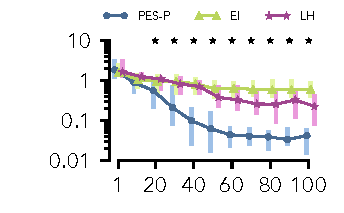
\includegraphics[width = \textwidth]{y_err2_legend}
        \vspace{-20pt}\caption{2 dimensions, $\lambda = 0.1$}\label{fig:y_err2}
    \end{subfigure}
    \begin{subfigure}[b]{0.24\textwidth}
    	\centering
        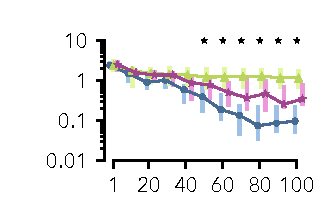
\includegraphics[width = \textwidth]{y_err3}
        \vspace{-20pt}\caption{3 dimensions, $\lambda = 0.2$}\label{fig:y_err3}
    \end{subfigure}
    \begin{subfigure}[b]{0.24\textwidth}
    	\centering
        \vspace{10pt}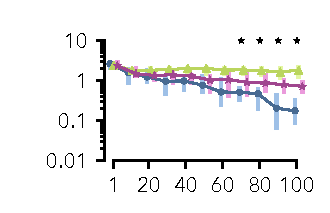
\includegraphics[width = \textwidth]{y_err4}
        \vspace{-20pt}\caption{4 dimensions, $\lambda = 0.3$}\label{fig:y_err4}
    \end{subfigure}
    \begin{subfigure}[b]{0.24\textwidth}
    	\centering
        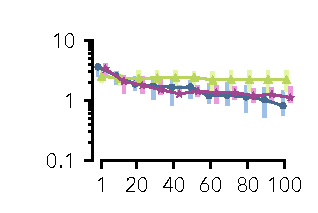
\includegraphics[width = \textwidth]{y_err5}
        \vspace{-20pt}\caption{5 dimensions, $\lambda = 0.4$}\label{fig:y_err5}
    \end{subfigure}
    \vspace{0.1in}
    \begin{subfigure}[b]{0.24\textwidth}
        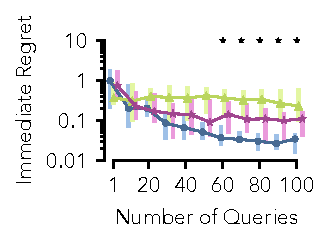
\includegraphics[width = \textwidth]{y_err3LQR}
        \vspace{-20pt}\caption{LQR 3 dim}\label{fig:LQR_3}
    \end{subfigure}
    \begin{subfigure}[b]{0.24\textwidth}
    	\centering
        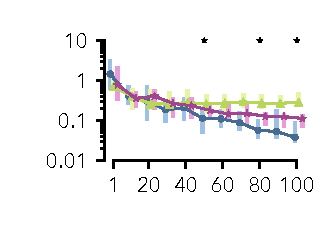
\includegraphics[width = \textwidth]{y_err4LQR}
        \vspace{-20pt}\caption{LQR 4 dim}\label{fig:LQR_4}
    \end{subfigure}
    \begin{subfigure}[b]{0.24\textwidth}
    	\centering
        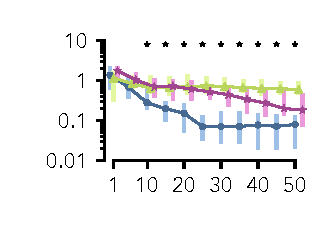
\includegraphics[width = \textwidth]{y_err2Neuro}
        \vspace{-20pt}\caption{Biped Walking  2 dim}\label{fig:Neuro_2}
    \end{subfigure}
    \begin{subfigure}[b]{0.24\textwidth}
    	\centering
        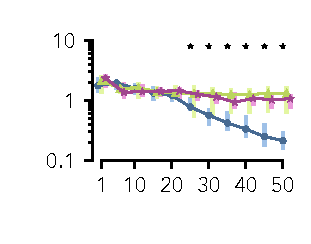
\includegraphics[width = \textwidth]{y_err3Neuro}
        \vspace{-20pt}\caption{Biped Walking 3 dim}\label{fig:Neuro_3}
    \end{subfigure}
    \caption{Performance of predictive entropy search with preferences (PES-P),
    expected improvement (EI), and Latin hypercube random sampling (LH) for
    optimizing random objective functions sampled from a GP (a-d), and tuning
    feedback control parameters of random linear systems (e-f) and a biped
    walking model (g-h). Shown are the median and interquartile range over 20
    trials of the immediate regret (IR) against the number of preference
    queries. Black stars indicate iterations for which PES-P achieves
    statistically significant stochastic reductions in IR compared to both EI
    and LH according to one-sided Mann-Whitney $U$ tests $(p <
    0.05)$.}\label{fig:y_err_sim}
\end{figure*}

\subsubsection{Optimizing Randomly Generated Objective Functions}

To avoid inducing bias by hand-engineering test functions, we first evaluate the
algorithm on random synthetic objective functions. We generate objective
functions on the domain $x \in {[-1, 1]}^D$ by sampling a vector of 500 function
values from a GP prior with a quadratic mean, $\mu(x) = - x^\tn{T} x$, and
isometric squared exponential covariance $\funcil{k}{x_i,x_j} = \exp
\left(\frac{-1}{2 \lambda} x_i^T x_j \right)$. We use a quadratic mean function
to bias the function distribution away from those that have their optimum on a
boundary of the domain, as these functions are easier to optimize. We continue
to generate the rest of the function as it is optimized by conditioning the GP
on the 500 seed values and all function values sampled during the optimization.
We assume the mean of the final function distribution is the true objective
function. To simulate more realistic situations, we provide the algorithms with
noisy preferences from the sampled function values ($\sigma^2 = 0.1$).

Figures~\ref{fig:y_err_sim}a-d show the immediate regret for two to five
dimensional problems with $\lambda$, the length scale of the kernel, scaling
from 0.1 to 0.4 as the dimensionality of the problem increases. On two to four
dimensional problems, PES-P outperforms EI and LH by achieving statistically
significant reductions in IR\@. However, as the dimensionality increases, it
takes more iterations for this advantage to become apparent. In the five
dimensional case, there is no significant difference between PES-P and LH,
likely due to $M=12$ samples of $x_m^*$ being insufficient and the difficulty of
accurately sampling $x_m^*$ in higher dimensions.

\subsubsection{Tuning Controllers for Random Linear Systems}
Next, we test the ability of PES-P to optimize simple control systems by
optimizing the feedback gains $K$ for $D$-dimensional single-input linear
systems $\dot{\xi} = A \xi + Bu$ with feedback $u = K \xi$. We sample the
elements of the $A$ matrix from the standard normal distribution while $B =
{[0_{1 \times (D-1)}, 1]}^\tn{T}$. We assume a quadratic instantaneous cost
resulting in the objective function
\begin{equation}
    f(K) = - \int_0^{t_f} \xi_K^\tn{T}(t) (Q + K^T R K) \xi_K(t) dt,
\end{equation}
where $\xi_K(t)$ is the evolution of the state under the control policy $K$ and
a fixed initial condition $\xi_0$, $Q = I_{D \times D}$ and $R = 1$. To obtain a
finite search domain, we find the stable range of parameters by varying the
elements of the true optimal control parameters $K^*$ one at a time while
keeping other elements constant. We scale and shift this region to map to the
domain ${[-1, 1]}^D$. Finally, we use the Automatic Relevance Determination
Gaussian Kernel and optimize the hyperparameters at each iteration by maximizing
the posterior probability of the hyperparameters under a gamma
hyperprior~\citep{chu2005preference,
williams2006gaussian}. In order to apply a consistent noisy preference model
$(\sigma^2 = 0.1)$ across all sampled systems, we transform all objective values
by first mapping them through $-\log(-f(K))$ and then shifting and scaling the
values by the mean and range of the values of $10^D$ randomly sampled
controllers. 

Figures~\ref{fig:y_err_sim}e and~\ref{fig:y_err_sim}f show the resulting
optimization performance on three and four dimensional systems. In the 3
dimensional case, PES-P achieves a lower median IR than LH after 30 iterations.
This difference becomes significant after 60 iterations. In the 4 dimensional
case, PES-P significantly outperforms LH after 50 iterations, but the
significance of this improvement is sporadic as the iterations continue. A
possible reason for the reduced performance difference between PES-P and LH in
the LQR problem as compared to the random objective function problems is the
existence of hard-to-optimize flat regions in the LQR objective functions. This
suggests that PES-P may be more well suited for problems that have clear
optimum.
\subsubsection{Tuning Control Parameters of a Walking Model
    }\label{sec:sim_neuro}
In the third case, we test the ability of PES-P to optimize the feedback gains
for a neuromuscular model of walking~\citep{thatte2016toward}, a system with a
complex non-linear controller addressing the specific application domain of
human locomotion. We perform two and three dimensional optimizations, in which
we tune the feedback gains for a subset of the model's muscle actuators.  We use
the negative cost of transport plus the distance walked over a 20 second time
span as the objective function. As in the previous linear systems example, we
obtain noisy preferences between parameters and optimize the hyperparameters at
every iteration.

Figures~\ref{fig:y_err_sim}g and~\ref{fig:y_err_sim}h show the performance of
PES-P, EI, and LH\@. In this example, PES-P achieves a significant reduction in
IR in just 10 iterations in the 2-dimensional case and in 25 iterations in the 3
dimensional case.  Furthermore, in the 3D case the PES-P's median solution is
approximately 10 times better than those found by EI or LH\@. 

\subsubsection{Tuning a Transfemoral Prosthesis from User Preferences} 
\begin{figure*}[t]
    \centering
    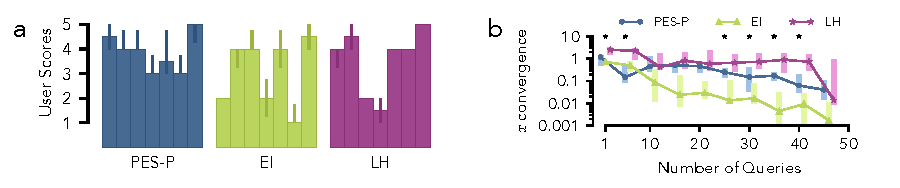
\includegraphics[width=\textwidth]{prosthesis_result_combined.pdf}
    \caption{Optimization of prosthesis control with user preferences. (a)
    Median and interquartile range of user scores achieved by PES-P, EI and LH
    after 50 iterations (total of 42 scores per algorithm: seven users times six
    scorings). (b) Median and interquartile range of convergence achieved by the
    three algorithms as measured by the Euclidean distance between the current
    and final estimates of the optimum. PES-P and LH achieve the same median
    score of 4 across all users but PES-P converges faster and more
    consistently. EI converges fastest but to a lower median score of
    3.}\label{fig:prosthesis_result}
\end{figure*}


In the last test case, we applied the three algorithms to optimize the control
parameters for a powered transfemoral prosthesis given real user preferences.
Specifically, a neuromuscular model similar to the one used
in~\cref{sec:sim_neuro} controls the prosthesis and we optimize the strengths
of three virtual knee muscles of this control~\citep{thatte2016toward}. 

We performed this test in a pilot study with seven healthy users. They walked
on a treadmill and wore the powered prosthesis with a modified knee brace
(compare~\citep{thatte2016toward}). We allowed all users an hour-long session to
acclimate to the device, during which they experienced a variety of controller
conditions. On a second day, we optimized the prosthesis parameters using the
three algorithms (PES-P, EI, and LH) in a random order, for 50 iterations each.
During an iteration, the users walked with two parameter settings chosen by the
algorithm (each for 10 seconds) and then indicated which setting they
preferred. After completing the three optimizations, the users walked with the
optimum parameters identified by each algorithm (in a random order) for fifteen
seconds and then rated each optimum on a 1 (bad) to 5 (good) scale. We repeated
the scoring procedure six times to cover all possible orderings of the three
optima.

\Cref{fig:prosthesis_result} summarizes the results from the optimizations with
user preferences. PES-P and LH achieved median user scores of 4 while EI
achieved a median score of 3 (Fig.~\ref{fig:prosthesis_result}a). In addition,
PES-P, LH, and EI achieved mean scores of 4.0, 3.5, and 3.1, respectively (not
shown). The gap between the mean and median scores for LH implies that LH does
not achieve high scores as consistently as PES-P. A second observation is that
PES-P converged faster than LH to the optimum as measured by the distance
between its current and final estimates, $\lVert \tilde{x}_n^* - \tilde{x}_N^*
\rVert$ (Fig.~\ref{fig:prosthesis_result}b).  Meanwhile, EI tended to converge
fastest, but to lower scoring parameters on average
(Fig.~\ref{fig:prosthesis_result}a).

\subsection{Discussion and Conclusion}\label{sec:tuning_discussion}
We presented a new optimization algorithm (PES-P) that extends Predictive
Entropy Search to preference feedback. The algorithm addresses two key problems
frequently encountered in system optimization. First, it circumvents the often
difficult process of parameterizing and learning an objective function by
directly querying users for preferences between pairs of parameters. Second, the
algorithm minimizes the required number of hardware experiments by employing
Bayesian optimization techniques that ensure the queries maximize the
information gained about the location of the optimum. Moreover, unlike previous
approaches for preference learning on robotic systems~\citep{wilson2012bayesian,
jain2013learning}, PES-P does not require a model of the system.

Our experiments show that the proposed algorithm outperforms baseline
algorithms. In most of the simulation experiments PES-P found optima that
achieved higher objective values than those found by the expected improvement
method (EI) or by random comparisons via Latin hypercubes (LH)
(\cref{fig:y_err_sim}). In the prosthesis experiment, PES-P outperformed EI and
achieved final scores similar to LH with faster convergence
(\cref{fig:prosthesis_result}). These results suggest the proposed algorithm can
help engineers optimize some types of human-in-the-loop robotic systems more
accurately, efficiently, and consistently. 

The reason why PES-P outperformed EI is likely due to the former's explicit
consideration of how the limited, noisy information obtained from a preference
query will affect the knowledge about potential objective function optima. The
acquisition function (\cref{eq:acquisition_orig}) recognizes that preferences
become more uncertain the closer two sample points are to each other. EI, on the
other hand, does not reason about noisy preferences and, instead, still assumes
it can sample values (\cref{eq:expected_improvement}). Consequently, EI ignores
the distance between sample points, which often leads to a greedy strategy that
solicits preferences between adjacent points. While this strategy can resemble
gradient ascent with convergence to local optima in a noise-free optimization,
it often failed in our simulated and real experiments characterized by noisy
observations. Note, however, that such limitations were not observed by Brochu
and colleagues~\citep{eric2008active}, who successfully used EI with preferences
to optimize parameters for a graphics application, possibly because the
associated visual task produced less noisy responses than did our simulations or
prosthesis walking task. 

Several modifications could improve the PES-P algorithm. First, using a non-zero
prior mean function governed by a set of hyperparameters could embed specific
knowledge about the problem to speed up optimization. To improve efficiency in
this way, \citep{brochu2010bayesian} details an approach for learning
hyperpriors that could be integrated with PES-P.  Second, integrating more
varied user feedback may also help improve the algorithm. For example, ``I don't
know'' responses could imply that the function values at two points are similar,
absolute good and bad ratings could encourage the algorithm to more quickly
explore promising control polices and avoid bad ones, derivative observations
could indicate the user prefers more or less of a parameter, and better than all
seen so far feedback could more clearly identify optimal parameters. Third, when
asking users to compare the optima achieved by the three algorithms, we had them
walk with each parameter set for 15 seconds and then give a rating for all
three. Subjects seemed able to recall and compare the performance of all three
parameter sets with ease. Therefore, moving forward, we should use comparisons
between three optima instead of pairwise comparisons as it will provide more
data per unit of time. Fourth, a greedier selection strategy may help improve
the performance of the algorithm in practice, as it will more quickly identify
good parameters even if they are suboptimal. With these four changes, the
algorithm may be able to tackle higher dimensional problems. Finally, we should
investigate is including time as a dimension in the GP to account for user
adaptation to the robotic system. This may allow us to eliminate the hour-long
adaptation session on the first day of our study. 

\hypertarget{sec:appendix}{\section*{Appendix}}

To obtain $X^*$ (line 5,~\cref{alg:pesp}), we sample $M$ functions from the
posterior by approximating $\prob{\vecf{f}[\tn{t}]|D_n}$ using Bayesian linear
regression with Fourier features (as outlined in~\citep{hernandez2014predictive})
and sampling $M$ feature weight vectors. As the Fourier features have analytic
derivatives, we can optimize each linear function using a second order method
with multiple restarts.

We approximate conditioning the predictive distribution on $x^*$ via three
constraints: 
\begin{description} 
    \item[C1] $x^*$ is a local maximum. $\nabla f|_{x^*} = 0$ and the
    Hessian of the objective function is negative definite by imposing
    $\func{diag}{\nabla \nabla f|_{x^*}} < 0$ and $\func{upper}{\nabla
    \nabla f|_{x^*}} = 0$. We group $\nabla f|_{x^*} = 0$ and
    $\func{upper}{\nabla \nabla f|_{x^*}} = 0$ into constraint C1.1 and
    $\func{diag}{\nabla \nabla f|_{x^*}} < 0$ into constraint C1.2.

    \item[C2] $x^*$ is preferred to current training points, $f(x^*) >
    f(x_k^\tn{a}) \textrm{ and }  f(x^*) > f(x_k^\tn{b}), \ \forall k \in [1,
    n]$.

    \item[C3] $x^*$ is preferred to new training points, $f(x^*) >
    f(x_{n+1}^\tn{a})$ and $f(x^*) > f(x_{n+1}^\tn{b})$.  
\end{description}

We precompute the effects of contraints C1 and C2 before evaluation of
$\funcil{\alpha}[n]{x^\tn{a}, x^\tn{b}}$. To impose C1 and C2, we first divide
their components into two groups: $\vecf{c} = [\nabla f|_{x^*}^\tn{T}, \
\func{upper}{\nabla \nabla f|_{x^*}}^\tn{T}]^\tn{T}$ and $\vecf{f}' =
[\vecf{f}^\tn{T},\ \func{diag}{\nabla \nabla f|_{x^*}}^\tn{T},\
f(x^*)]^\tn{T}$. Note $\tn{C1.1} \implies \vecf{c} = 0$. We write the predictive
distribution of the objective function at test points $\vecf{f}[\tn{t}]$ given
constraints C1 and C2 as
\begin{align}
    \prob{\vecf{f}[\tn{t}]|D_n, \tn{C1},\tn{C2}} = 
    \int\prob{\vecf{f}[\tn{t}]| \vecf{f}', \tn{C1.1}}  
    \prob{\vecf{f}' | D_n, \tn{C1}, \tn{C2}} \tn{d}\vecf{f}'.
    \label{eq:predictive_w_constraints}
\end{align}
We use Bayes rule to evaluate the second term in the integral, $\prob{\vecf{f}'
| D_n, \tn{C1}, \tn{C2}} = \frac{\prob{D_n , \tn{C1.2}, \tn{C2} |\vecf{f}'}
\prob{\vecf{f}'| \tn{C1.1}}}{\prob{D_n, \tn{C1.2}, \tn{C2} | \tn{C1.1}}}$. We
form the prior term $\prob{\vecf{f}'|\tn{C1.1}}$ by conditioning the joint
distribution, $\prob{\vecf{c}, \vecf{f}'}$  on $\tn{C1.1}$ given by $\vecf{c} =
0$. $\prob{\vecf{f}'|\vecf{c}} = \mathcal{N}\left( \vecf{f}'|
\Sigma_\tn{cf'}^\tn{T} \Sigma_\tn{cc}^{-1} \vecf{c}, \Sigma_\tn{f'f'} -
\Sigma_\tn{cf'}^\tn{T} \Sigma_\tn{cc}^{-1} \Sigma_\tn{cf'} \right)$ implies
$\prob{\vecf{f}'|\vecf{c}=0} = \mathcal{N}(\vecf{f}'| 0, \Sigma_\tn{f'|c})$.

We implement the likelihood term by adding extra factors to the likelihood
in~\cref{eq:bayes_rule} that impose soft constraints representing C1.2 and C2.
For C1.2 we use the penalty term $\prob{[\nabla \nabla f|_{x^*}]_{dd} <
0 | \nabla \nabla f|_{x^*}} = \Phi(-[\nabla \nabla
f|_{x^*}]_{dd}/\sigma_\tn{h})$ and for C2 we add more preference relations
between $x^*$ and all training points. 
\begin{fullwidth}
\begin{align}
    \prob{D_n, \tn{C1.2}, \tn{C2}, |\vecf{f}'} 
        &=\left[ \prod_{k=1}^n \prob{x_k^\tn{a} \succ x_k^\tn{b} 
            | f(x_k^\tn{a}), f(x_k^\tn{b})} 
        \prob{x^* \succ x_k^\tn{a} | f(x^*), f(x_k^\tn{a})} 
        \prob{x^* \succ x_k^\tn{b} | f(x^*), f(x_k^\tn{b})} \right] \notag\\
        &\quad \times  \prod_{d=1}^D \prob{{[\nabla \nabla f|_{x^*}]}_{dd} < 0
            | {[\nabla \nabla f|_{x^*}]}_{dd}} \notag \\
        &= \left[ \prod_{k=1}^n \Phi(q_k) \Phi(q_k^{\tn{a}*}) 
                \Phi(q_k^{\tn{b}*}) \right]
            \prod_{d=1}^D \Phi(q_d^\tn{h})
\end{align}
\end{fullwidth}
Where $q_k^{\tn{a}*} = \frac{f(x^*) - f(x_k^\tn{a})}{\sqrt{2} \sigma}$ and
$q_k^{\tn{b}*} = \frac{f(x^*) - f(x_k^\tn{b})}{\sqrt{2} \sigma}$ and $q_d^{h} =
\frac{-[\nabla \nabla f|_{x^*}]_{dd}}{\sigma_h}$. We use Laplace's approximation
to approximate $\prob{\vecf{f}' | D_n, \tn{C1}, \tn{C2}}$ as Gaussian,
\begin{align}
    \prob{\vecf{f}' | D_n, \tn{C1}, \tn{C2}} \approx \mathcal{N}\left(\vecf{f}'|
        \vecf{f}'_{\tn{MAP}}, {\left(\Sigma_\tn{f'|c}^{-1} +
        \Lambda_{f'_\tn{MAP}} \right)}^{-1} \right),
    \label{eq:rprime_given_constraints}
\end{align}
where $\vecf{f}'_\tn{MAP} = \arg \min_{\vecf{f}'} -\log
\prob{\vecf{f}' | D_n, \tn{C1}, \tn{C2}}$ and $\Lambda_\tn{f'_{MAP}}$ is the
Hessian of $-\log \prob{D_n , \tn{C1.2}, \tn{C2}|\vecf{f}'}$ evaluated at
$\vecf{f}'_\tn{MAP}$.

We compute the first term in~\cref{eq:predictive_w_constraints},
$\prob{\vecf{f}[\tn{t}]|\vecf{f}', \tn{C1.1}}$ by conditioning the joint
distribution $\prob{\vecf{c}, \vecf{f}', \vecf{f}[\tn{t}]}$
on $\vecf{f}'$ and $\vecf{c} = 0$,
\begin{fullwidth}
\begin{align}
    \prob{\vecf{f}[\tn{t}] | \vecf{f}', \vecf{c}=0} = \mathcal{N} \left(
        \vecf{f}[\tn{t}] | 
        \left( \Sigma_\tn{ct}^\tn{T} B + \Sigma_\tn{f't}^\tn{T} D \right) 
            \vecf{f}', \Sigma_\tn{tt} - 
        \begin{bmatrix} 
            \Sigma_\tn{ct}^\tn{T} & \Sigma_\tn{f't}^\tn{T} 
        \end{bmatrix}
        \begin{bmatrix}
            A & B \\ C & D
        \end{bmatrix}
        \begin{bmatrix} \Sigma_\tn{ct} \\ \Sigma_\tn{f't} \end{bmatrix} \right),
        \label{eq:P_r_given_rprimec}
\end{align}
\end{fullwidth}
where,
    $\begin{bmatrix}
        A & B \\ C & D
    \end{bmatrix} = 
    \begin{bmatrix}
        \Sigma_\tn{cc} & \Sigma_\tn{cf'} \\ \Sigma_\tn{cf'}^\tn{T} &
        \Sigma_\tn{f'f'}
    \end{bmatrix}^{-1}$.
We can substitute~\cref{eq:P_r_given_rprimec}
and~\cref{eq:rprime_given_constraints} into~\cref{eq:predictive_w_constraints}
to yield the predictive distribution subject to constraints $C1$ and $C2$.
\begin{fullwidth}
\begin{align}
    \prob{\vecf{f}[\tn{t}]|D_n, \tn{C1}, \tn{C2}} = &\mathcal{N}
        \left( \vecf{f}[\tn{t}] | 
    (\Sigma_\tn{ct}^\tn{T} B + \Sigma_\tn{f't}^\tn{T} D) 
        \vecf{f}'_\tn{MAP}, \Sigma_\tn{tt} - 
        \begin{bmatrix} 
            \Sigma_\tn{ct}^\tn{T} & \Sigma_\tn{f't}^\tn{T} 
        \end{bmatrix}
        \begin{bmatrix}
            A & B \\ C & D
        \end{bmatrix}
        \begin{bmatrix} 
            \Sigma_\tn{ct} \\ \Sigma_\tn{f't} 
        \end{bmatrix} \right. \notag \\
        & \left. + \left( 
            \Sigma_\tn{ct}^\tn{T} B + \Sigma_\tn{f't}^\tn{T} D\right)
        {\left(\Sigma_\tn{f'|c}^{-1} + \Lambda_\tn{f'_{MAP}}\right)}^{-1}
        {\left(\Sigma_\tn{ct}^\tn{T} B + \Sigma_\tn{f't}^\tn{T} D
        \right)}^\tn{T} \right).
    \label{eq:pred_dist_constrain_xstar}
\end{align}
\end{fullwidth}
We obtain $\prob{\vecf{f}[\tn{t}]|D_n, \tn{C1}, \tn{C2}, \tn{C3}}$ by
analytically conditioning \cref{eq:pred_dist_constrain_xstar} on the single
inequality $f(x_m^*) > (f(x^\tn{a}) + f(x^\tn{b}))/2$ using the method detailed
in~\citep{xu2010estimation}. Finally, using~\cref{eq:predic_pref_w_constraint} we
can compute the predictive distributions of preferences given the locations of
$x_m^*$.

To optimize $\funcil{\alpha}[n]{x^\tn{a}, x^\tn{b}}$ (line 7,~\cref{alg:pesp})
we construct its gradient by evaluating $\prob{\vecf{f}[\tn{t}] | D_n}$ and
$\prob{\vecf{f}[\tn{t}] | D_n, \tn{C1},\tn{C2},\tn{C3}}$ at test points
$x^\tn{a}$ and $x^\tn{b}$ as well as points offset by $\delta_x = \pm 0.001$
along each dimension. We then optimize $\alpha_n(x^\tn{a}, x^\tn{b})$ via
gradient ascent.

\chapter{Proposed Work}

\section{Evaluation of Neuromuscular Transfemoral Prosthesis Control}

\section{Optimizing Prosthesis Control using Preferneces}

\section{Learning Trip Recovery Policies}
\label{sec:proposed_trip_recovery}

\section{Proposed Work Summary and Timeline}


% The back matter contains appendices, bibliographies, indices, glossaries, etc.

\backmatter

\bibliography{references}
\bibliographystyle{plainnat}

\end{document}
